\chapter{Un Islam Français est possible}

\begin{marginfigure}
\centering

\includegraphics[width=0.91222in,height=0.54469in]{ImageIslamFrance/media/image6.png}
\caption{
Normalien, agrégé de géographie, \textbf{Hakim El Karoui} a enseigné à
l'université Lyon II avant de rejoindre le cabinet du Premier ministre
en 2002, où il était chargé de ses discours. Après un passage à Bercy,
il rejoint, en 2006, la banque Rothschild où, avec Lionel Zinsou, il
anime la practice Afrique. En 2011, il rejoint le cabinet de conseil en
stratégie Roland Berger où il est co-responsable de l'Afrique et du
conseil au gouvernement français. En 2016, il fonde sa propre société de
conseil stratégique Volentia. Hakim El Karoui est aussi essayiste (il a
publié trois livres chez Flammarion qui traitent de questions
économiques et géopolitiques) et entrepreneur social (il a créé le club
du XXIe siècle, les Young Mediterranean Leaders et est avec Bariza
Khiari à l'origine de « l'appel des 41 », paru le 31 juillet 2016 dans
le JDD). L'analyse des données de l'enquête inédite, réalisée dans le cadre de ce
rapport, a été effectuée par \textbf{Antoine Jardin}, docteur en science
politique et ingénieur de recherche au CNRS.}
\end{marginfigure}



\subsection{Avant-Propos}


Pourquoi travailler sur l'islam en 2016 ? Parce que la violence qui
s'est déchaînée en son nom en France, contre des Français, ne peut
rester sans réponse. Il faut engager des changements profonds dans
l'organisation de cette religion pour lui donner les moyens de lutter
contre le fondamentalisme religieux qui crée un terreau favorable au
terrorisme. Pourquoi travailler sur l'islam en cette pré-campagne
électorale ? Parce que l'on ne peut se satisfaire des sempiternelles
polémiques sur l'inscription des signes d'appartenance islamique dans
l'espace public, -- le burkini étant le dernier exemple\ldots-- comme
seules réponses politiques au djihadisme et au fondamentalisme : tout
cela traduit surtout un sentiment d'impuissance et nourrit crispations
et angoisses au sein de la société française.

Ces peurs sont renforcées par la méconnaissance générale des musulmans
français : qui sont-ils ? Quels rapports entretiennent-ils avec la
religion ? Avec les autorités religieuses ? Les rares connaissances dont
nous disposons étaient imprécises et ne se fondaient que sur des
estimations. C'est pour porter remède à cette situation que l'Institut
Montaigne a conduit avec l'IFOP une enquête inédite, soumise à la plus
grande rigueur méthodologique et au strict respect de la législation en
vigueur. \paragraph{Que nous enseigne l'IFOP ?} Que le nombre de musulmans en France
est moins important que ne l'avancent bon nombre de chiffres
fantaisistes : ils représentent 5,5 \% de la population de plus de 15
ans en métropole. Que cette population est nettement plus jeune que la
moyenne nationale. Qu'elle est aussi moins qualifiée, même si une classe
moyenne et une élite émergent clairement. Cette large enquête atteste
également qu'une majorité des musulmans de France a un système de valeur
et une pratique religieuse qui s'insèrent sans heurts majeurs dans le
corpus républicain et national. Elle montre enfin que nombreux -- mais
minoritaires -- sont les -- jeunes -- Français de confession musulmane,
qui se définissent d'abord et avant tout par leur identité religieuse,
suivant une logique implacable : 
\begin{quote}
    « plus vous êtes fondamentaliste, plus
vous êtes musulman et donc plus vous êtes vous-même ».
\end{quote} En arrière-plan,
une relation complexe avec la France, l'attrait du fondamentalisme
religieux étant un moyen pour eux d'exprimer une forme de révolte contre
une société qui les rejette ; c'est du moins très largement leur
perception. Malgré les difficultés à comparer les évolutions dans le
temps, en raison de la rareté des chiffres disponibles et des
contraintes méthodologiques, il ne fait pas de doute que cette tendance
est en augmentation sensible depuis dix ans.

Deux réalités très différentes donc : une majorité silencieuse, très
souvent pratiquante mais sans conflit majeur avec les normes de la
société française, d'une part ; une minorité, attirée par le
fondamentalisme, qui utilise l'islam pour dire sa révolte, d'autre part. On peut le déplorer, s'en féliciter, vouloir le
combattre ou le respecter, ce fait social est bien réel. Il faut le
traiter, dans le contexte qui est le nôtre - celui d'une violence
terroriste et sans limite perpétrée au nom de l'islam, qui rend
angoissant pour une majorité de Français le mouvement d'affirmation
identitaro-religieux voire théologico-politique qui est à l'œuvre.

Or, le système mis en place en 2003 avec la création du Conseil français
du culte musulman (CFCM) a montré ses limites :


\begin{itemize}
\item
  (i) influence des États étrangers à qui la France a sous-traité une
  forme de contrôle social et sécuritaire ;
\item
  (ii) incompréhension face aux mutations d'un islam de plus en plus
  identitaire, porté par des jeunes garçons et des jeunes filles, très
  souvent Français de naissance, que ne comprennent pas les responsables
  des institutions actuelles -- quasiment tous des hommes, souvent âgés
  de plus de 60 ans, nés à l'étranger ;
\item
  (iii) incapacité, enfin, à intervenir face au phénomène rampant de la
  radicalisation religieuse alors que théories du complot, antisémitisme
  et postures victimaires fleurissent chez ceux-là même qui trouvent
  dans un islam autoritaire -- voire radical -- un moyen d'affirmation.
\end{itemize}


De nombreux problèmes ont fait obstacle, jusqu'à présent, et ont entravé
les évolutions de l'organisation de l'islam en France :


\begin{itemize}
\item
  géopolitiques, d'abord, car l'organisation de l'islam de France se
  trouve enchâssée dans l'écheveau complexe des relations de la France
  avec les pays du Maghreb et la Turquie ;
\item
  organisationnels, ensuite, parce que, malgré les inquiétudes relatives
  au communautarisme musulman, la « communauté musulmane en France »
  n'existe tout simplement pas : ni sentiment d'appartenance, ni
  intérêts communs identifiés, ni capacité d'action groupée. Depuis
  trente ans, les ministres de l'Intérieur successifs ont d'ailleurs
  tous échoué à trouver un interlocuteur représentatif ;
\item
  financiers également, car malgré certains financements venus de pays
  étrangers « amis » (le Maroc, la Turquie, l'Algérie et l'Arabie Saoudite), l'islam est sous-financé et pâtit, par ailleurs, d'un manque de transparence qui
entrave sa capacité à collecter les dons des fidèles et qui est dommageable pour sa réputation ;
\item
  institutionnels, enfin, car il faut que le gouvernement français fasse
  bien davantage confiance aux musulmans de France et notamment aux
  élites qui ont émergé ou sont en train de le faire. À cet égard, la
  nomination de Jean-Pierre Chevènement à la tête de la Fondation pour
  l'islam de France n'est pas un signe encourageant et elle a suscité,
  malgré les qualités de cet ancien Ministre, incompréhension et
  déception. Il ne serait sans doute venu à l'esprit de personne de le
  désigner pour une telle mission auprès des autres grandes religions
  présentes sur le sol national.
\end{itemize}


Cinq mutations majeures doivent pourtant être engagées :


\begin{itemize}
\item
  « sortir l'islam de France de la minorité » en comprenant enfin que
  les musulmans ne sont ni des mineurs qu'il faut mettre sous tutelle ni
  des irresponsables toujours divisés qu'il faut considérer avec
  commisération sans jamais les croire capables d'agir efficacement :
  cela a été souvent l'attitude des pouvoirs publics, confrontés il est
  vrai à des querelles incessantes de représentants plus ou moins auto-
  proclamés de l'islam en France. Cet objectif repose sur deux
  impératifs :

  \begin{itemize}
  \item
    mettre fin à la tutelle - longtemps acceptée voire encouragée par la
    France - d'États étrangers, qui ne tolèreraient en aucune manière
    sur leur sol ce qu'ils pratiquent en France : imagine-t-on la
    France, ou l'Italie qui vit sous régime concordataire, financer le
    culte catholique dans tel ou tel pays musulman et le cabinet du
    Premier ministre envoyer le texte des prêches chaque dimanche aux
    desservants français établis dans ces pays ? C'est pourtant ce qui
    se passe en France aujourd'hui. Cette action sera réussie quand les
    flux financiers venus de ces pays ne seront plus dirigés vers « leur
    » communauté, mais de façon claire et transparente, vers une
    organisation reconnue dont les moyens financiers seront destinés à
    l'ensemble des musulmans de France, quelle que soit leur origine ;
  \item
    faire émerger de nouveaux cadres, religieux et laïcs, nés en France,
    soucieux de prendre en main une communauté embryonnaire et de
    répondre aux très nombreux défis auxquels sont confrontés les
    musulmans de France. La solution pour y parvenir, c'est de leur
    donner une légitimité institutionnelle en les associant à la
    création et à la gouvernance de la Fondation pour l'islam de France
    et à l'association musulmane pour un islam de France ;
  \end{itemize}

\item
  assurer à l'islam de France des ressources financières transparentes,
  destinées à un usage collectif, afin de structurer une véritable
  organisation de l'islam, de salarier les imams et de répondre au fait
  social indéniable que constitue « la nouvelle fierté islamique » de
  nombreux musulmans de France, qui font de l'islam un objet moins
  religieux qu'identitaire. La solution, c'est une redevance sur le
  halal et des institutions reconnues capables d'attirer des dons;
\item
  travailler de façon efficace à la formulation et à la diffusion
  d'interprétations de l'islam alternatives aux discours de fermeture,
  de séparation et de soumission;
\item
  contribuer, autant que le permet la loi de 1905, à la lutte contre le
  discours fondamentaliste, notamment \emph{via} le financement de la
  formation -- culturelle - et du travail des aumôniers dans tous les
  lieux fermés (écoles, prisons, armées, établissements hospitaliers,
  etc.) et \emph{via} l'enseignement de l'arabe à l'école publique (dans
  un contexte où cet enseignement se diffuse très rapidement dans les
  mosquées et les écoles coraniques, du fait, notamment, de l'absence
  d'offre de formation à l'école) ;
\item
  une réflexion doit, enfin, être engagée sur l'absence de l'islam du
  concordat qui régit encore la relation entre les cultes et l'État en
  Alsace-Moselle. Il en va de l'égalité entre les citoyens et de la
  capacité de l'État de créer une faculté de théologie capable de
  travailler rapidement sur des interprétations religieuses en phase
  avec la réalité française contemporaine ;
\item
  lever les ambiguïtés qui pèsent sur certaines pratiques locales (baux
  emphytéotiques, carrés confessionnels, garanties d'emprunt) pour
  garantir aux musulmans que ces pratiques juridiques sont conformes à
  la Constitution.
\end{itemize}


Pour y arriver, il faut tenir compte de la nouvelle réalité de l'islam
dans notre pays : les musulmans sont majoritairement nés en France et
aujourd'hui Français pour les trois-quarts d'entre eux. Autre évolution
sociologique importante : si les ouvriers, les employés et les chômeurs
sont surreprésentés par rapport à la moyenne nationale, une nouvelle
élite bien formée et bien insérée dans le monde professionnel est en
train d'émerger.

Construire un islam français est donc possible mais, ô combien difficile
! Il faudra assumer, parfois, la crispation des uns et des autres et
avoir suffisamment bien préparé ces évolutions afin qu'elles puissent
aboutir. Il faudra se préparer à répondre
aux polémiques venues de tous les camps tant cette question est
sensible, complexe et sujette à manipulation en ces temps de campagne
électorale. Il faudra être prêt à bousculer les conservatismes et les
idées reçues de toutes parts.

C'est pourquoi l'État devra s'investir au plus haut niveau pour faire
émerger cette nouvelle organisation de l'islam français, car il a encore
un rôle à jouer pour faciliter les changements avant de se retirer
ensuite, conformément au principe de laïcité. L'enjeu est essentiel :
c'est notre cohésion nationale qu'il faut préserver, et, c'est aussi,
pour les musulmans, l'occasion d'inventer une nouvelle modernité
religieuse.


\subsubsection{Un portrait des musulmans de France}

Voir des Français -- chrétiens, musulmans, juifs, athées -- mourir « au
nom de l'islam » : cette réalité est devenue la nôtre depuis les
attentats perpétrés par Mohamed Merah en 2012. Les événements de ces
deux dernières années, violents, terribles, différents par leurs cibles,
leur envergure mais pas par les réactions qu'ils ont suscitées, se
nouent les uns aux autres dans une déflagration sordide. La peur et la
haine dominent. Les esprits, notamment politiques, sont troublés et
confus : le piège tendu par les djihadistes -- attiser la haine contre
tous les musulmans pour encourager ces derniers à les rejoindre -- reste
ouvert, béant. Avec le risque qu'un jour il ne se referme sur la société
française.

Une brève analyse des couvertures des principaux magazines
hebdomadaires1 montre que l'islam est invariablement présenté comme
porteur de violence et de haine : il s'agit là exactement de ce que
veulent les djihadistes qui, par leurs actions, orientent cette
couverture médiatique2. Une quarantaine de numéros des six magazines les
plus vendus en France ont ainsi placé un sujet lié à l'islam en
couverture au cours des douze derniers mois ; en moyenne, chaque
semaine, un magazine a dédié sa « une » à l'islam. La rhétorique
visuelle de ces numéros recourt d'ailleurs souvent aux mêmes éléments :
sur un fond sombre s'accumulent des photos d'hommes en armes, de leaders
enturbannés, de sabres ; larges polices, couleurs vives, contrastent
avec des fonds sombres. Le champ lexical des enquêtes policières est
mobilisé : il faut trouver les \emph{« complices »}, les \emph{«
cerveaux »}, les

\emph{« armées souterraines »}. Lorsqu'il s'agit d'étudier les relations
de l'État et de l'islam, le champ lexical est celui de la défaite, de la
faiblesse. Les « unes » portant sur des régimes se revendiquant de
l'islam (l'Iran ou l'Arabie Saoudite) utilisent le vocabulaire de la
menace et de la peur. Une tonalité commune se dessine dans le traitement
de ces sujets, dont les champs lexicaux et les visuels sont ceux de la
menace, de l'alarme et de l'inquiétude. L'islam reste à déchiffrer. Les
enjeux géopolitiques et les courants extrémistes accaparent la
représentation. Il convient de remarquer qu'un seul numéro sur ces
quarante s'intéresse au quotidien des musulmans français\sn{\emph{M le magazine du Monde,} « La religion, la mode, le travail, les
garçons, paroles de jeunes filles voilées », 21/05/2016.}.


Cette tendance a commencé avec la révolution islamique en Iran qui a
inauguré l'âge des revendications politiques entremêlées de référents
religieux. Depuis les années 1980, les crises survenues en Palestine, en
Jordanie, au Liban, en Irak, en Algérie, en Bosnie, en Afghanistan, en
Tchétchénie, en Syrie, en Libye et au Yémen sont peu à peu devenues «
islamiques ». Les « printemps arabes » et leurs conséquences, la montée
de l'islam politique, sont venus confirmer que tout sujet concernant des
pays de population musulmane pouvait désormais donner lieu à une lecture
par le prisme du religieux.

Depuis la fin des années 1980, la France débat de l'islam et de son
rapport avec la République et la laïcité. Le premier débat portait sur
le voile en 1989, suivi par ceux de 1993 et de 2003. Avant les
commentaires sur la présence ou non d'une composante musulmane dans
l'imaginaire des émeutes des banlieues en automne 2005, qui ont précédé
les discussions sur l'identité nationale, alimentées par
l'interprétation des propos de tel ou tel intellectuel musulman, les
saillies de représentants d'ONG salafistes sur les plateaux de
télévision, les prêches d'imams radicaux, etc. L'islam ne semble exister
que dans trois cadres: les relations internationales et géopolitiques ;
les attentats terroristes et les faits de société liés à la montée du
salafisme ou de l'islamisme politique ; ainsi que leur relation avec les
valeurs laïques.

Face au danger terroriste, l'État se doit d'apporter une réponse
sécuritaire. C'est évidemment légitime mais cela ne peut être suffisant.
Il faut également répondre par la connaissance aux défis que les
événements de 2015 et de 2016 ont fait naître, afin d'éclairer les
débats à venir d'éléments solides et objectifs. On bute alors sur la
méconnaissance de la population musulmane française : qui sont-ils ? Que
pensent-ils ? Nul ne le sait vraiment en raison des carences de la
statistique publique dès lors qu'il s'agit de religion4. Pourtant, des
enquêtes d'opinion sont légales et possibles. C'est pourquoi nous avons
lancé une grande enquête d'opinion sur les musulmans de France. Les
objectifs sont simples : il faut mieux les connaître, afin d'être à même
ensuite de proposer des solutions susceptibles d'accélérer la sereine
insertion de la majorité silencieuse, mais aussi des mesures destinées à
combattre le fondamentalisme, tout en ramenant le plus grand nombre
possible de musulmans -- souvent des jeunes -- tentés par l'intégrisme
vers des croyances et des idées en phase avec les valeurs républicaines.



\section{Un portrait des musulmans de France}


\paragraph{La méthodologie de l'Enquête}

Ce document présente les principaux résultats d'une enquête réalisée
sur les opinions et les pratiques sociales des personnes musulmanes, et
issues de familles musulmanes, en France. Il s'agit d'une enquête
expérimentale, pionnière en France, dont il convient d'utiliser les
résultats avec précaution et mesure. Elle se distingue par sa volonté
d'interroger la population musulmane dans son ensemble, et non plus
seulement les musulmans parmi la population immigrée.

La question religieuse ne peut être abordée via le recensement général
de l'INSEE, elle ne peut pas l'être non plus par les méthodes de sondage
traditionnelles qui, lorsqu'il s'agit d'interroger des musulmans de
France, ciblent généralement les quartiers où résident un nombre
important d'immigrés. C'est pourquoi nous avons élaboré une
méthodologie, qui vise à extraire d'un vaste échantillon représentatif
de la population résidant en France métropolitaine -- 15 459 personnes
de 15 ans et plus ont été interrogées -- un échantillon spécifique de
personnes musulmanes ou de culture musulmane ; elles représentent 1 029
individus, parmi lesquels 874 se définissent comme « musulmans ». Cette
enquête respecte les principes scientifiques et déontologiques de
l'enquête par sondage. Elle achoppe sur les mêmes difficultés : la marge
d'erreur moyenne d'un sondage effectué auprès d'un échantillon de 1 000
personnes est d'environ 3 \%, celle inhérente à l'analyse d'un
sous-groupe dans ce même échantillon augmente sensiblement et peut
s'élever entre 6 et 8 \%.Les enseignements qu'elle indique reflètent un
état de l'opinion à l'instant de sa réalisation et non pas une
prédiction. Si les calculs sont solides et rigoureux scientifiquement,
les analyses présentées constituent l'une des manières possibles de
traiter les données de cette enquête. Il existe bien évidemment d'autres
méthodes et d'autres choix statistiques, qui pourraient donner lieu à
des résultats différents.

Toutefois, la méthodologie utilisée nous semble constituer le meilleur
compromis afin de produire des résultats fiables. Dans un souci de
transparence, nous publions

\mn{La représentativité de l'échantillon global a été assurée par la
méthode des quotas au regard :


\begin{itemize}
\item
  De critères sociodémographiques (sexe de l'individu, âge de
  l'individu) ;
\item
  De critères socioprofessionnels (profession de l'individu) ;
\item
  De critères géographiques (région administrative, taille d'unité
  urbaine, proportion d'immigrés dans la commune ou du quartier (IRIS)
  de résidence) ;
\item
  De critères civiques (nationalité) ;
\end{itemize}


Ces quotas ont été définis à partir des données du recensement de
l'INSEE pour la population âgée de 15 ans et plus résidant en métropole
(RP-INSEE 2012).}
l'ensemble des procédures techniques employées à chaque étape, ce qui
permet ainsi à n'importe quel autre utilisateur de logiciels
statistiques de pouvoir vérifier et de reproduire nos résultats.
L'analyse d'une enquête si importante ne peut être réalisée au moyen
d'une « boite noire » ; l'usage de techniques vérifiables s'inscrit, au
contraire, en cohérence avec le respect des normes académiques les plus
exigeantes à ce jour.

Cependant, l'analyse complète et approfondie d'une enquête si riche
exige davantage de temps. Les résultats présentés constituent une
première analyse exploratoire, qui devra être précisée et affinée
ultérieurement. Le caractère novateur de cette enquête vise aussi à
identifier les apports et les difficultés méthodologiques liées à
l'étude quantitative des populations religieuses minoritaires dans la
société française ; certaines de ces difficultés nous ont conduits à
faire des choix techniques et pratiques, pour lesquels nous avons
toujours eu à l'esprit la recherche de la précision et de l'exactitude
des résultats.



\subsection{Les caractéristiques socio démographiques des musulmans de France}

La principale tendance sociodémographique de l'islam en France est la
prégnance croissante de la seconde religion du pays auprès des jeunes
générations. Cette dynamique s'explique par la conjugaison de deux
facteurs : la transmission intergénérationnelle d'une part et les
conversions d'autre part.


\begin{itemize}
\item
  
  Le premier apport démographique provient de la transmission
  intergénérationnelle de la religion chez les descendants d'une
  immigration issue de pays musulmans. Cette transmission n'est pas
  toujours linéaire et il s'agit également, parfois, d'un retour au
  religieux des enfants et des petits-enfants issus de familles dans
  lesquelles le religieux était peu important.
  
\item
  
  Le second apport démographique provient des conversions à l'islam
  parmi les personnes n'ayant eu aucun rapport familial avec l'islam au
  cours des générations précédentes.
  
\end{itemize}

\begin{figure}
    \centering
    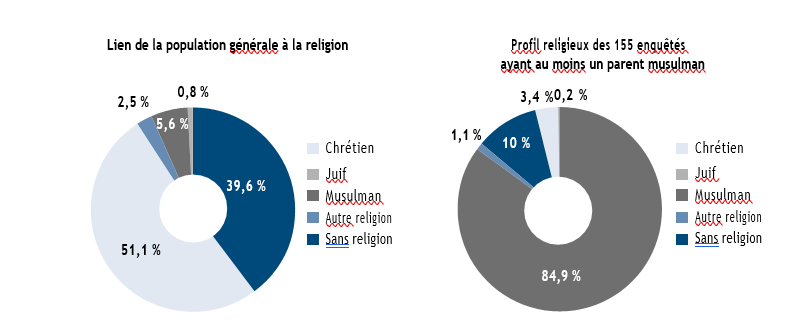
\includegraphics[width=\textwidth]{ImageIslamFrance/profilreligieux.png}
    \caption{Lien de la population générale à la religion Profil religieux
des 155 enquêtés ayant au moins un parent musulman}
    \label{fig:my_label}
\end{figure}

Ces deux dynamiques se combinent et se complètent.

Si 5,6 \% de la population totale des plus de 15 ans7 se déclarent
musulmans dans notre enquête8, cette proportion dépasse les 10 \% chez
les moins de 25 ans.

À l'inverse, deux tendances majeures se dessinent au sein du reste de la
population française :


\begin{itemize}
\item
  
  le déclin persistant de l'affiliation à la chrétienté ;
  
\item
  
  l'accroissement du nombre de personnes qui se déclarent « sans
  religion ».
  
\end{itemize}


Parmi les plus de 75 ans, près de trois répondants sur quatre se
déclarent chrétiens et moins de 20 \% indiquent n'avoir aucune religion,
contre respectivement 30 \% et près de 50 \% chez les moins de 30 ans.


\hypertarget{duxe9mographie}{%
\subparagraph{Démographie}\label{duxe9mographie}}


D'après les résultats de notre enquête, les personnes qui se déclarent
musulmanes représentent 5,6 \% de la population métropolitaine.

Cette proportion est approximative, dans la mesure où la technique du
sondage induit nécessairement des marges d'erreurs qui rendent difficile
l'estimation précise et fiable de ce chiffre ; l'absence de données
officielles, qui permettraient de procéder à un redressement
sociodémographique, contribue également à ce manque de
précision. Cependant, ce résultat est proche d'autres estimations
existantes et apparaît donc pertinent.

Dans l'échantillon initial de 15 459 personnes, plus de 47 \% des plus
de 15 ans se déclarent « chrétiens », 37 \% « sans religion », 6 \% ont
refusé de répondre à cette question et un peu plus de 3 \% s'affilient à
une autre religion minoritaire que l'islam. Ces chiffres rappellent que,
si l'islam est la seconde religion de France métropolitaine, elle est
démographiquement très minoritaire\sn{5 \% des individus interrogés ont refusé de répondre à cette question.}. La structure socioprofessionnelle
de la population qui se définit comme musulmane est marquée par une
surreprésentation des milieux populaires et des populations éloignées de
l'emploi :


\begin{itemize}
\item
  
  plus de 24 \% des musulmans déclarés sont ouvriers ;
  
\item
  
  plus de 22 \% sont employés ;
  
\item
  
  30 \% des musulmans sont inactifs non retraités. Ces personnes ne
  figurent pas dans les statistiques du chômage tel qu'il est calculé en
  France ; elles n'occupent pas d'emploi mais ne sont pas enregistrées
  comme demandeuses d'emploi. Cette catégorie inclut, en revanche, les
  lycéens et étudiants, mais aussi les jeunes à la recherche d'un
  premier emploi10 ;
  
\item
  
  seuls 4,5 \% sont cadres. À titre de comparaison, les cadres
  représentent 10 \% des personnes qui se déclarent « sans religion » et
  plus de 8 \% des chrétiens. \emph{A contrario,} les inactifs non
  retraités ne pèsent que 14 \% et 9,9 \% respectivement dans ces deux
  groupes. Si l'on raisonne en termes de taux d'incidence, les musulmans
  représentent 2,8 \% des cadres mais plus de 10 \% des ouvriers, 7 \%
  des employés et 13,5 \% des inactifs non retraités.
  
\end{itemize}


Cela peut s'expliquer en partie par la pyramide des âges de ce groupe
social, où les jeunes sont significativement plus nombreux. Les
musulmans de l'échantillon sont âgés, en moyenne, de 35,8 ans contre 53
ans pour les chrétiens et 43,5 ans pour les personnes sans religion.

Cet échantillon possède la particularité d'inclure à la fois la
population se déclarant musulmane, et celle qui ne se déclare pas comme
telle mais dont l'un des parents au moins est musulman. Ce dernier
groupe représente 15 \% de la population de l'enquête. Ces personnes
possèdent des ascendants directs musulmans, mais se positionnent
subjectivement comme en dehors de cette religion.






72 \% des répondants se déclarent musulmans lorsque leurs deux parents
sont également musulmans ; 2,7 \% sont musulmans alors que seul leur
père est musulman ; 2,8 \% alors que seule leur mère est musulmane. La
très grande majorité des musulmans, s'inscrit donc dans une transmission
religieuse directe au sein d'une famille dans laquelle les deux parents
sont musulmans.

Cependant, il ne s'agit pas d'un modèle de transmission unique ; ainsi
7,5 \% des personnes se déclarant comme musulmanes déclarent qu'aucun de
leurs parents n'est musulman. Les musulmans sans aucun parent musulman
sont plus nombreux que les musulmans dont seul l'un des deux parents est
musulman. Ce chiffre peut correspondre, de façon schématique, à ce que
l'on considère comme les conversions à l'islam.

Par ailleurs, bien que la religion islamique soit transmise en principe
de façon patrilinéaire, les musulmans dont seul le père est musulman ne
sont pas plus nombreux que ceux dont la seule la mère est musulmane.

Enfin, comme les non-musulmans représentent 15 \% des enquêtés, les
trajectoires de « sortie » de la religion musulmane -- ou de
désaffiliation --apparaissent deux fois plus importantes que les
trajectoires d'entrée ; prenant à rebours les représentations faisant de
l'islam une religion attirant massivement des individus \emph{a priori}
éloignés de cette tradition.

La croissance démographique de l'islam en France suit davantage le
mouvement des générations dans la période post-coloniale que celui d'un
courant idéologique.



\paragraph{Nationalité}

Les données de l'enquête révèlent que 50 \% des enquêtés sont français
de naissance, 24 \% sont français par acquisition et 26 \% sont de
nationalité étrangère. Parmi les Français, nombreux sont les individus
qui possèdent également une autre nationalité, en lien avec leur
trajectoire migratoire ou celle de leurs parents.

La très grande majorité des musulmans étrangers sont originaires du
Maghreb, d'Afrique Subsaharienne ou de Turquie. Les citoyens de ces pays
représentent en effet 23 \% des musulmans de France et représentent plus
de 88 \% des individus ne détenant pas la nationalité française.





\paragraph{Pays d'origine}



\textbf{Pays de naissance du père}
Le père des enquêtés est, dans près de 90 \% des cas, né hors de France.
Ce chiffre semble très élevé, mais il apparaît, dans nos données, plus
faible que dans les résultats de l'enquête \emph{Trajectoire et
Origines} (TeO), conduite par l'INED auprès de la population des
migrants et descendants de migrants de moins de 50 ans en 2008.
Rappelons ici que notre choix méthodologique porte sur l'ensemble de la
population résidant en France, et pas uniquement sur les personnes de
nationalité française. L'Algérie et le Maroc sont les principaux pays
d'origine, avec respectivement 31 \% et 20 \%. La Tunisie représente 8
\% des origines paternelles, les autres pays d'Afrique un peu plus de 15
\% et la Turquie environ 5 \%.


\textbf{Pays de naissance de la mère}
Les mères des enquêtés présentent un profil d'origine nationale
comparable. Il existe cependant des variations significatives : dans
près d'un cas sur cinq (17 \%), les mères sont nées en France, soit 7
points de plus que les pères.

Le croisement des pays de naissance du père et de la mère révèle la
puissance de l'endogamie nationale :


\begin{itemize}
\item
  
  72 \% des enquêtés dont le père est né en France ont aussi une mère
  née en France ;
  
\item
  
  88 \% des personnes ayant un père né en Algérie ont une mère née dans
  le même pays ;
  
\item
  
  91 \% des personnes dont le père est né au Maroc ont une mère née au
  Maroc ;
  
\item
  
  les taux d'endogamie sont comparables pour les personnes originaires
  de Tunisie, de Turquie, ou des autres pays d'Afrique.
  
\end{itemize}

\textbf{Pays de naissance de l'enquêté}
Les 1 029 répondants eux-mêmes sont nés en France dans plus d'un cas sur
deux.

Pour ceux qui sont nés à l'étranger :


\begin{itemize}
\item
  
  14 \% sont nés en Algérie ;
  
\item
  
  près de 13 \% au Maroc ;
  
\item
  
  11 \% principalement en Afrique subsaharienne ;
  
\item
  
  et près de 5 \% en Tunisie.
  
\end{itemize}
\paragraph{Origine sociale}



\begin{figure}
    \centering
    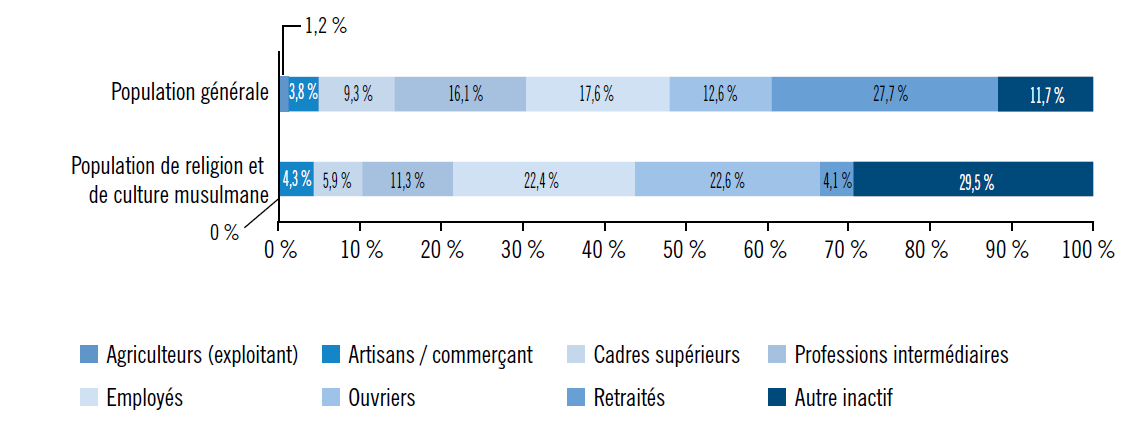
\includegraphics[width=\textwidth]{ImageIslamFrance/OrigineSociale.png}
    \caption{Origine sociale des enquêtés et de la population générale}
    \label{fig:my_label}
\end{figure}

Cette enquête permet également de mesurer la position sociale d'origine
des enquêtés, c'est-à-dire la profession et la catégorie
socioprofessionnelle (PCS) de leur responsable de famille au moment de
l'enquête. Si cette information nous éclaire sur le milieu social
d'origine des enquêtés, en revanche, elle ne nous renseigne pas sur leur
situation individuelle.

De plus, la nomenclature des PCS échoue à saisir la condition sociale
réelle des individus, dans la mesure où parmi la catégorie des personnes
inactives, elle ne distingue ni les étudiants ni les militaires du
contingent ni les « inactifs divers » de moins de 60 ans (non-retraités)
sans activité professionnelle ni les chômeurs n'ayant jamais exercé
d'activité.

On constate une prééminence nette des catégories sociales populaires et
des personnes inactives et une forte sous-représentation des classes
supérieures du salariat (cadres et professions intellectuelles
supérieures).

Les 874 enquêtés qui se déclarent musulmans sont ainsi sous-représentés
parmi les professions intermédiaires (8 \% contre 14,1 \% dans la
population générale) et les cadres et professions intellectuelles
supérieures (4 \% contre 9 \% parmi la population générale) ; et
surreprésentés parmi les ouvriers (24 \% contre 13,1 \%) et les inactifs
(38 \% contre 16,1 \%).




\paragraph{Diplôme}


Alors que leur position sociale d'origine est très modeste, les
musulmans de France se hissent à des niveaux de qualification qui se
rapprochent de la moyenne nationale.

Les personnes titulaires d'un diplôme de niveau BAC + 2 représentent
environ 12 \% de l'échantillon, les titulaires de diplômes plus élevés
20 \% -- dont la moitié possède un titre de niveau BAC +5.
\begin{figure}
    \centering
    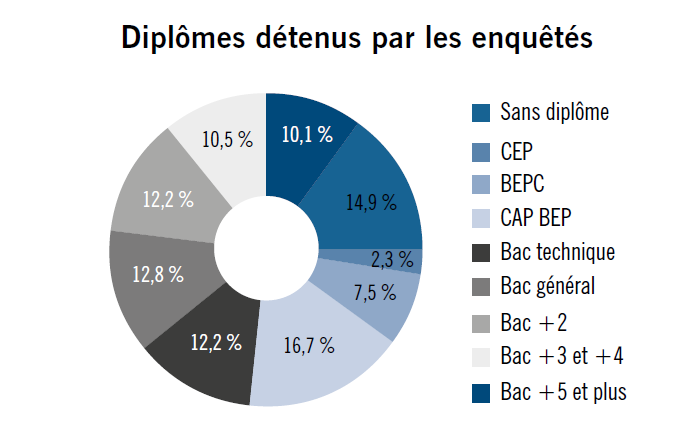
\includegraphics[width=\textwidth]{ImageIslamFrance/Diplome.png}
    \sidecaption{Diplômes détenus par les enquêtés}
    \label{fig:my_label}
\end{figure}



Cependant, une part importante des enquêtés présente également de plus
faibles niveaux de formation :


\begin{itemize}
\item
  
  près de 15 \% ne possèdent aucun diplôme ;
  
\item
  
  environ 25\% ont un niveau inférieur au BAC.
  
\end{itemize}


Cela est le signe d'une polarisation sociale de la population musulmane,
marquée par un accès assez large à l'enseignement supérieur, d'une part,
mais également par la marginalisation scolaire d'une importante
minorité, d'autre part.


Statut dans l'emploi


Si une large part des 1 029 répondants est inactive, la majorité des
personnes actives occupe un emploi stable. Ainsi, plus de 55 \% occupent
un CDI et 10 \% sont fonctionnaires. En revanche, en raison de leur
position sociale plus défavorisée, la précarité touche une part
significative de la population de culture musulmane : plus de 12 \% est
en CDD et plus de 8 \% est en intérim.




\begin{figure}
    \centering
    \includegraphics[width=\textwidth]{ImageIslamFrance/Emploi.png}
    \caption{Statut dans l'emploi des enquêtés}
    \label{fig:my_label}
\end{figure}


\paragraph{Pyramide des âges}


La pyramide des âges témoigne de la jeunesse de la population musulmane
de France. L'âge moyen des répondants est de 35 ans et 75 \% d'entre eux
ont moins de 45 ans.

Ces résultats peuvent être liés à l'évolution démographique de la
population musulmane en France, mais peuvent également être inhérents
aux difficultés que rencontrent fréquemment les instituts de sondage
pour joindre les personnes les plus âgées, notamment parmi les migrants
âgés résidant en France.

Cependant, un nombre important de répondants de plus de 50 ans a pu être
interrogé, complétant en cela l'information sur une population qui ne
figurait pas dans le spectre de l'enquête TeO conduite par l'INSEE et
l'INED.





\subsection{Typologie des musulmans selon leur religiosité}


Nous avons sélectionné plusieurs variables permettant de définir le
rapport au religieux, afin de construire une typologie au moyen d'une
Analyse en Composantes Principales (ACM).

Cette typologie permet de déterminer les dimensions latentes, qui
sous-tendent les rapports au religieux parmi les 1 029 enquêtés. Afin de
rendre ces résultats plus compréhensibles, nous avons ensuite opéré une
classification pour identifier un petit nombre de groupes, parmi les
personnes qui se déclarent musulmanes ou dont les parents sont
musulmans. La construction de l'ACM et de la typologie sont détaillées
en annexe. Là encore, cette typologie n'est que l'une des typologies
possibles. De plus, les critères techniques retenus pour la division des
classes peuvent varier. Aussi, il convient de ne pas attacher trop
d'importance au périmètre et au poids absolu des différentes classes
mais davantage à la structuration générale des opinions et des
attitudes.


\paragraph{Description des classes construites}


Cette typologie permet de distinguer six classes, ordonnées de la
catégorie des individus les plus modérés aux individus les plus
autoritaires :


\begin{itemize}
\item
  La \textbf{première catégorie (18 \% des effectifs) est celle des
  individus les plus éloignés de la religion.} Ils sont favorables à la
  laïcité, ne formulent aucune revendication d'expression religieuse
  dans la vie quotidienne, qu'il s'agisse du monde du travail ou de
  l'école, ne souhaitent pas de nourriture halal à la cantine et sont
  très largement d'accord avec l'idée que la laïcité permet de pratiquer
  librement sa religion.
\item
  La \textbf{deuxième catégorie (28 \% des effectifs) partage les mêmes
  valeurs.} Les individus qui la composent sont d'accord avec
  l'interdiction de la polygamie et avec l'idée que la loi de la
  République passe avant la loi religieuse. \textbf{Elle se distingue
  par un attachement plus fort à la consommation de nourriture halal et
  une partie de ses membres est favorable à l'expression religieuse au
  travail.}
\item
  La \textbf{troisième catégorie (13 \% des effectifs) est plus
  ambivalente.} Elle s'oppose au niqab et à la polygamie, mais elle
  conteste l'idée selon laquelle la laïcité permet de pratiquer
  librement sa religion. Sans être radicale, elle critique le modèle
  républicain, \emph{a minima} dans ses modalités d'application.
  \textbf{Une forte minorité de ces membres souhaite d'ailleurs pouvoir
  exprimer sa religion sur son lieu de travail.}
\end{itemize}



\begin{itemize}
\item
  La \textbf{quatrième catégorie (12 \% des effectifs) se distingue de
  la troisième par une plus grande acceptation de la laïcité. En
  revanche, elle critique massivement l'interdiction de la polygamie en
  France} tout en condamnant absolument le niqab, rejeté par 95 \% des
  membres de ce groupe. Cette catégorie réunit beaucoup de musulmans
  étrangers résidant en France.
\item
  La \textbf{cinquième catégorie (13 \% des effectifs) représente les
  individus qui présentent des traits autoritaires :} 40 \% de ses
  membres sont favorables au port du niqab, à la polygamie, contestent
  la laïcité et considèrent que la loi religieuse passe avant la loi de
  la République. Dans leur immense majorité, les membres de ce groupe ne
  considèrent pas que la foi appartienne à la sphère privée, ils sont
  d'ailleurs majoritairement favorables à l'expression de la religion au
  travail.
\item
  La \textbf{sixième catégorie (15 \% des effectifs) se distingue de la
  cinquième en prônant une vision plus « dure » des pratiques
  religieuses.} En revanche, elle valorise la foi comme un élément privé
  et non comme un élément public. Presque tous ses membres valorisent le
  port du niqab et près de 50 \% contestent la laïcité tout en étant
  favorables à l'expression de la religion sur le lieu de travail.
\end{itemize}


Ces six catégories racontent trois histoires différentes :


\begin{itemize}
\item
  \textbf{Groupe 1 (catégories 1 et 2 représentant 46 \% des musulmans
  de France) sont soit totalement sécularisés soit en train d'achever
  leur intégration dans le système de valeurs de la France
  contemporaine, qu'ils contribuent d'ailleurs à faire évoluer par leurs
  spécificités religieuses.} Ils ne renient pas pour autant leur
  religion, souvent identifiée au halal, et ont une pratique religieuse
  nettement plus régulière que la moyenne nationale ;
\item
  \textbf{Groupe 2 (catégories 3 et 4) : il est plus composite et
  s'inscrit clairement dans une position intermédiaire. Fiers d'être
  musulmans,} les individus qui le composent revendiquent la possibilité
  d'exprimer leur appartenance religieuse. Très pieux (la charia a une
  grande importante pour eux, sans passer devant la loi de la
  République), ils sont souvent favorables à l'expression de la religion
  au travail, et ont très largement adopté la norme halal comme
  définition de « l'être musulman ». Ils rejettent très clairement le
  niqab et la polygamie et acceptent la laïcité ;
\item
  \textbf{Groupe 3 (catégories 5 et 6) : il est le plus problématique.
  Il réunit des musulmans qui ont adopté un système de valeurs
  clairement opposé aux valeurs de la République.} Majoritairement
  jeunes, peu qualifiés et peu insérés dans l'emploi, ils vivent dans
  les quartiers populaires périphériques des grandes agglomérations. Ils
  se définissent davantage par l'usage qu'ils font de l'islam pour
  signifier leur révolte que par leur conservatisme. Si certains
  considèrent
\end{itemize}




que la laïcité leur permet de vivre librement leur religion\sn{11 « La laïcité permet aux musulmans de pratiquer librement leur
religion »
\begin{itemize}
\item
  Plutôt d'accord • Plutôt pas d'accord • Refuse de répondre • Ne sait
  pas
\end{itemize}} ou
considèrent que la foi est une affaire privée\sn{12 « Diriez-vous que la foi religieuse est pour vous d'abord quelque
chose de privé ? »
\begin{itemize}
\item
  Oui, tout à fait • Oui, plutôt • Non, plutôt pas • Non, pas du tout •
  Refuse de répondre • Ne sait pas
\end{itemize}}, on peut davantage y
lire une attitude de retrait et de séparation vis-à-vis du reste de la
société que la compréhension de ce que signifie la laïcité. \textbf{28
\% des musulmans de France} peuvent être regroupés dans ce groupe qui
mélange à la fois des attitudes autoritaires et d'autres que l'on
pourrait qualifier de « sécessionnistes ». \textbf{L'islam est un moyen
pour eux de s'affirmer en marge de la société française.}

À partir de ces éléments, il est possible d'étudier les caractéristiques
sociodémographiques des groupes identifiés selon la typologie du rapport
à la religion que nous venons d'établir.


\paragraph{Description sociodémographique des groupes}


\textbf{Effet de l'âge}

L'effet de l'âge est l'un des mécanismes les plus puissants en matière
d'analyse du rapport au religieux. \textbf{Le groupe 1, le plus éloigné
de la religion, est très peu représenté parmi les jeunes générations.}
S'il représente toujours près de la moitié des individus chez les plus
de 40 ans, il ne concerne plus qu'un tiers des répondants les plus
jeunes.

Ce mouvement est compensé par la croissance du groupe 3, \textbf{le plus
rigoriste religieusement et le plus autoritaire, qui passe d'environ 20
\% de la population des plus de 40 ans à près de 50 \% chez les cohortes
les plus jeunes.}

En revanche, le poids du groupe intermédiaire (groupe 2) est à la fois
faible et stable quelles que soient les cohortes étudiées.






Il n'est pas ici possible de vérifier statistiquement qu'il existe un
effet d'âge et non un effet de génération, mais ce scénario apparaît
comme le plus plausible. \textbf{Le mouvement à l'œuvre semble se
caractériser par une intensification de l'identité religieuse des
nouvelles cohortes (par rapport à leurs aînés au même âge).} L'hypothèse
alternative invite à considérer qu'au cours de leur vie les personnes de
culture musulmane vivant en France s'éloignent des formes les plus
rigoristes de rapport au religieux. Si cette hypothèse ne peut pas
\emph{a priori} être rejetée ici, elle paraît peu probable au regard des
autres travaux publiés sur ces questions.


Effet de la catégorie socio-professionnelle


L'effet de la catégorie socio-professionnelle sur le rapport au
religieux est, là aussi, significatif.

\textbf{Les personnes qui appartiennent aux catégories sociales les plus
favorisées (Cadres, Professions intermédiaires) sont nettement
surreprésentées dans le groupe 1, et sous représentées dans le groupe 3}
-- le plus autoritaire. En revanche, le lien identitaire fort à l'islam
est surreprésenté dans les milieux populaires, chez les ouvriers et les
employés, et plus fortement encore parmi les inactifs, qui regroupent
notamment les jeunes n'ayant jamais occupé d'emploi et les étudiants.

Les logiques d'âge et de classe sociale se combinent et permettent
d'identifier le renforcement probable des attitudes religieuses
autoritaires parmi les jeunes et dans les catégories populaires de la
population musulmane résidant en France. \textbf{Ce mouvement n'est pas
spécifique aux jeunes musulmans des milieux populaires. Il s'observe
également chez les jeunes qui se définissent comme chrétiens ou sans
religion, mais s'exprime par d'autres opinions et comportements que
l'affiliation identitaire à l'islam.}

\begin{figure}
    \centering
    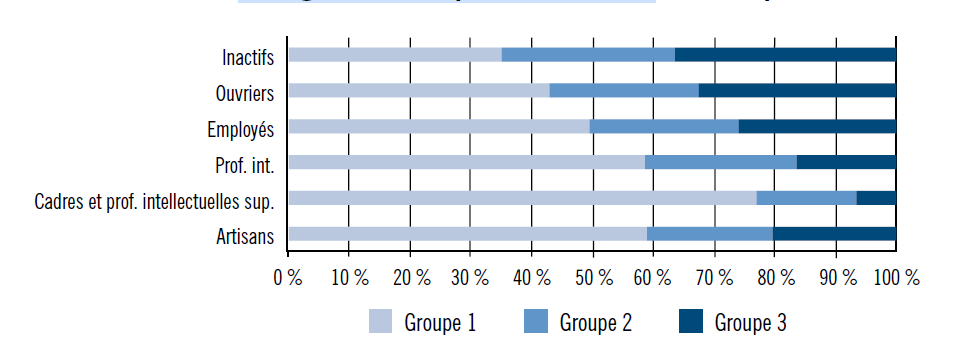
\includegraphics{ImageIslamFrance/CSP.png}
    \caption{Catégorie socio-professionnelle des enquêtés}
    \label{fig:my_label}
\end{figure}




\textbf{Effet du type d'activité
} L'analyse des effets du statut d'activité confirme cela. \textbf{Les
personnes les mieux insérées sont celles qui ont le plus de chance de
rejeter les attitudes les plus rigoristes dans le rapport à l'islam.}
Cela ne signifie en rien que la religion soit moins importante pour eux,
ou qu'ils soient « moins musulmans » que les autres. Les variations du
rapport au religieux, telles qu'identifiées dans cette typologie, sont
des différences de nature et non des différences de degré.


\begin{figure}
    \centering
    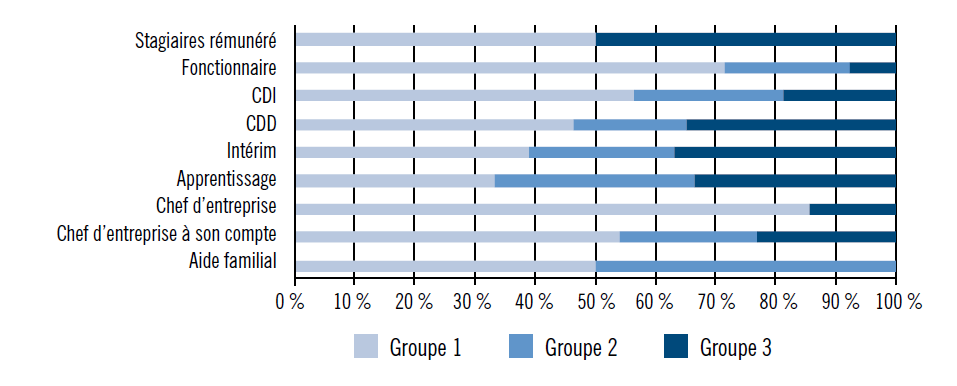
\includegraphics{ImageIslamFrance/activite.png}
    \caption{Activité exercée par les enquêtés des 3 groupes 
    Les chefs d'entreprises, les fonctionnaires et les salariés en CDI se
situent en dehors du groupe 3 dans plus de 80 \% des cas. En revanche,
\textbf{les personnes en position plus précaire (stagiaires, salariés en
intérim ou en CDD) sont celles qui, parmi les actifs, sont le plus
susceptibles d'appartenir aux groupes qui présentent les attitudes les
plus intransigeantes.}}
    \label{fig:my_label}
\end{figure}






Effet du genre


La comparaison entre les hommes et les femmes sur le rapport au
religieux indique que les femmes apparaissent légèrement surreprésentées
dans le groupe 3, mais ces écarts sont minimes une fois rapportés aux
dynamiques sociales et générationnelles. Ainsi, il existe davantage de
différences dans le rapport à l'islam entre une femme musulmane de 20
ans et une femme musulmane de 60 ans, qu'entre un homme et une femme du
même âge.

I. UN PORTRAIT DES MUSULMANS DE FRANCE


Influence du genre sur le rapport au religieux


Groupe 1 Groupe 2 Groupe 3 Femme Homme

\textbf{Effet du type de lien à l'islam}

Nous avons cherché à déterminer si ces dynamiques sont présentes chez
les seules personnes qui se déclarent musulmanes, ou si elles se
retrouvent également parmi les personnes dont l'un des deux parents est
musulman mais qui ne disent pas elles-mêmes musulmanes.


Répartition des enquêtés dans les 3 groupes


36,7 \%

Groupe 1 Groupe 2 Groupe 3 Musulman De culture musulmane

Les résultats peuvent paraître surprenants : \textbf{si les
non-musulmans présentent un rapport plus distancié au religieux que les
musulmans, l'écart est relativement mince.} C'est notamment le cas pour
le groupe 3, celui qui rassemble les plus autoritaires : près de 20 \%
des enquêtés qui se déclarent non-musulmans soutiennent les mêmes
positions.



Cette situation montre que l'islam est souvent davantage le support
d'une attitude de rébellion qu'une adhésion spirituelle qui entraînerait
une pratique particulièrement rigoriste.


Effet du type de lien à l'islam (2)


Pour affiner ce résultat, il est important de comparer les groupes selon
le rapport familial à l'islam (un parent, deux parents ou aucun parent
musulman). Les différences sont faibles et fragiles statistiquement,
cependant \textbf{il semble que ce soit les personnes converties
(musulmanes sans parent musulman) qui présentent les attitudes les plus
autoritaires.}

Il faut cependant nuancer ces éléments car ces profils sont minoritaires
en nombre dans tous les groupes sociaux14.


\begin{enumerate}
\def\labelenumi{\arabic{enumi}.}
\item ~
  \hypertarget{quelles-pratiques-de-lislam}{%
  \paragraph{QUELLES PRATIQUES DE L'ISLAM
  ?}\label{quelles-pratiques-de-lislam}}

  \begin{enumerate}
  \def\labelenumii{\arabic{enumii}.}
  \item ~
    \hypertarget{le-halal-et-les-normes-alimentaires}{%
    \subparagraph{Le halal et les normes
    alimentaires}\label{le-halal-et-les-normes-alimentaires}}
  \end{enumerate}
\end{enumerate}


La consommation de viande halal fait l'objet d'un intérêt important pour
les musulmans, qui l'identifient de plus en plus au simple fait d'être
musulman : être musulman, c'est être halal (par opposition à « haram »).
De fait, \textbf{de nombreuses représentations erronées circulent.
Ainsi, plus de 40 \% des répondants musulmans souscrivent à
l'affirmation selon laquelle la consommation de viande halal
constituerait l'un des 5 piliers de l'islam,} ce qui est évidemment
faux15.

70 \% des répondants déclarent « toujours » acheter de la viande halal,
22 \% en achètent « parfois » et seulement 6 \% « jamais ».

Comme l'ont montré plusieurs travaux depuis l'enquête \emph{Banlieue de
la République16}, la consommation de nourriture halal devient un
marqueur d'appartenance au groupe social des musulmans, y compris chez
les individus n'étant pas -- ou peu --

14 Les commentaires produits ici portent sur les niveaux relatifs des
différentes attitudes et non sur leur niveau absolu.

15 Les cinq piliers, dans le sunnisme, étant la profession de foi, la
prière, la zakat (soutien financier aux pauvres), le jeûne du mois de
Ramadan, et le pèlerinage à la Mecque une fois dans la vie pour ceux qui
en ont les moyens.

16 Gilles Kepel, \emph{Banlieue de la République,} 2011.


\begin{enumerate}
\def\labelenumi{\Roman{enumi}.}
\item
  UN PORTRAIT DES MUSULMANS DE FRANCE
\end{enumerate}


religieux. On décèle ici les signes d'un rapport au religieux qui se vit
d'abord par les normes et les pratiques sociales, et de façon secondaire
par les pratiques rituelles ou cultuelles.

Cette consommation halal est forte dans l'ensemble de la population
musulmane et

« d'origine » musulmane. Ainsi, huit répondants sur dix souscrivent à
l'affirmation selon laquelle les enfants devraient avoir la possibilité
de manger halal à l'école. Ce chiffre est moindre, mais reste très
élevé, chez les répondants de culture musulmane ne se déclarant plus
musulmans (67 \%).

Ce marqueur social semble s'être autonomisé de la référence religieuse :
la consommation halal est devenue normale -- au sens propre du terme. La
norme sociale dépend alors moins de la foi et de la théologie que d'un
mode de vie partagé.

Comme le montre le graphique suivant, il n'y a pas d'effet d'âge net sur
la consommation de nourriture halal parmi la population interrogée.
Ainsi, plus de 80 \%, toutes les classes d'âges confondues, déclarent
acheter « toujours » ou

« parfois » du halal. Et c'est logiquement que 80 \% des musulmans
interrogés souscrivent à l'affirmation suivante : \emph{« Les enfants
devraient pouvoir manger halal dans les cantines scolaires ».}

De façon analogue, le niveau de qualification ne semble pas avoir
d'influence nette sur la consommation de halal. La répartition est là
encore relativement homogène parmi l'ensemble des répondants.


Influence du niveau d'études des enquêtés sur leur consommation de halal


Jamais Parfois Toujours


\begin{longtable}[]{@{}
  >{\raggedright\arraybackslash}p{(\columnwidth - 16\tabcolsep) * \real{0.11}}
  >{\raggedright\arraybackslash}p{(\columnwidth - 16\tabcolsep) * \real{0.11}}
  >{\raggedright\arraybackslash}p{(\columnwidth - 16\tabcolsep) * \real{0.11}}
  >{\raggedright\arraybackslash}p{(\columnwidth - 16\tabcolsep) * \real{0.11}}
  >{\raggedright\arraybackslash}p{(\columnwidth - 16\tabcolsep) * \real{0.11}}
  >{\raggedright\arraybackslash}p{(\columnwidth - 16\tabcolsep) * \real{0.11}}
  >{\raggedright\arraybackslash}p{(\columnwidth - 16\tabcolsep) * \real{0.11}}
  >{\raggedright\arraybackslash}p{(\columnwidth - 16\tabcolsep) * \real{0.11}}
  >{\raggedright\arraybackslash}p{(\columnwidth - 16\tabcolsep) * \real{0.11}}@{}}
\toprule
\begin{minipage}[b]{\linewidth}\raggedright

Aucun

\end{minipage} & \begin{minipage}[b]{\linewidth}\raggedright

CEP

\end{minipage} & \begin{minipage}[b]{\linewidth}\raggedright

Brevet

\end{minipage} & \begin{minipage}[b]{\linewidth}\raggedright

CAP BEP

\end{minipage} & \begin{minipage}[b]{\linewidth}\raggedright

Bac Pro

\end{minipage} & \begin{minipage}[b]{\linewidth}\raggedright

Bac général

\end{minipage} & \begin{minipage}[b]{\linewidth}\raggedright

Bac +2

\end{minipage} & \begin{minipage}[b]{\linewidth}\raggedright

Bac +3/+4

\end{minipage} & Bac +5 \\
\midrule
\endhead
\begin{minipage}[t]{\linewidth}\raggedright

diplôme

\end{minipage} & & & & \begin{minipage}[t]{\linewidth}\raggedright

et technique

\end{minipage} & & & & et plus \\
\bottomrule
\end{longtable}




En ce qui concerne la question plus spécifique des repas halal proposés
dans les cantines scolaires, les résultats présentent également une
relative homogénéité parmi l'ensemble des 1 029 personnes interrogées.
On observe néanmoins que 35 \% des répondants titulaires d'un diplôme de
niveau bac+5 ou plus disent ne pas être d'accord avec la proposition «
les enfants devraient pouvoir manger halal dans les cantines scolaires
», alors que moins d'une personne sur cinq partage cette opinion parmi
le reste des enquêtés.


Influence du niveau d'études des enquêtés


\textbf{sur leur souhait de voir les cantines scolaires proposer de la
nourriture halal}

Pas d'accord D'accord

Aucun diplôme

CEP Brevet CAP BEP Bac Pro et technique


Bac général Bac +2 Bac +3/+4 Bac +5

et plus


\textbf{Ainsi, une majorité de musulmans consomme régulièrement du
halal. L'attachement à cette pratique n'est ni révélateur d'un rapport
plus radical à la religion ni un indicateur de fondamentalisme
religieux.}


\hypertarget{le-port-du-voile-quelles-motivations}{%
\subparagraph{Le port du voile : quelles motivations
?}\label{le-port-du-voile-quelles-motivations}}


Le port du voile est une question ancienne dans le rapport à l'islam en
France. C'est par la question du port du voile dans les établissements
scolaires que l'Union des Organisations islamiques de France (UOIF) est
apparue sur la scène médiatique et a touché une audience importante dans
les années 1990 et au début des années 2000. Plus récemment, de nombreux
débats ont eu lieu autour de l'interdiction du port du voile intégral
(loi de 2009), sur la possibilité d'une extension aux Universités de
l'interdiction du voile à l'école, adoptée en 2004, ou encore sur les
conditions de l'interdiction du port du voile dans les entreprises
(notamment avec l'affaire Baby Loup).


\begin{enumerate}
\def\labelenumi{\Roman{enumi}.}
\item
  UN PORTRAIT DES MUSULMANS DE FRANCE
\end{enumerate}


\textbf{Environ 60 \% des 1 029 enquêtés considèrent que les jeunes
filles devraient pouvoir porter le voile au collège et au lycée.} En
revanche, cette position n'est soutenue que par 37 \% des personnes de
culture musulmane -- dont les parents sont musulmans mais qui ne se
déclarent pas musulmanes. Ainsi, la question du voile reste nettement
plus clivante, y compris parmi les musulmans, que ne l'est celle de la
consommation de viande halal.

\textbf{Environ 65 \% des musulmans -- de religion ou de culture -- se
déclarent favorables au port du voile}17\textbf{,} et 24 \% sont
favorables au principe du port du voile intégral18. Dans les deux cas,
environ 10 \% des répondants adoptent une position de retrait individuel
en choisissant la réponse \emph{« c'est son choix, chacun fait ce qu'il
veut ».}

Contrairement à l'opinion dominante qui voudrait que les hommes soient
plus conservateurs que les femmes, le port du voile est rejeté par 26 \%
des hommes mais seulement par 18 \% des femmes. Les hommes sont
également plus enclins à déclarer que \emph{« chacun fait ce qu'il veut
».} \textbf{Ces résultats témoignent d'une adhésion idéologique d'une
part importante de la population féminine musulmane au port du voile,
allant jusqu'à l'acceptation du voile intégral (pour 28 \% des femmes).}

Cependant, l'approbation du port du voile ne signifie en rien que les
comportements des individus correspondent à la norme ainsi revendiquée,
sachant que le port du voile intégral est interdit dans l'espace public.
Peut-être peut-on lire dans ces résultats très élevés une forme de
provocation, suite notamment aux nombreux débats sur le port des signes
religieux musulmans dans l'espace public.

La pratique sociale la plus répandue reste le non-port du voile.
\textbf{Ainsi, les deux tiers des femmes de culture musulmane déclarent
ne pas porter le voile.} 57 \% déclarent ne l'avoir jamais porté et 8 \%
déclarent l'avoir déjà porté, mais ne plus le faire aujourd'hui19.

Environ 35 \% des répondantes déclarent porter le voile (tout le temps
ou de manière épisodique). Si ce chiffre semble en augmentation au
regard des enquêtes réalisées en 2003 sur ces questions (+ 11 points),
il reste très éloigné des 65 \% évoqués précédemment :

17 « Personnellement, êtes-vous favorable à ce qu'une femme porte le
voile -- le hijab ? »

18 « Personnellement, êtes-vous favorable à ce qu'une femme porte le
voile intégral -- niqab ou burqa ? »

19 Question posée : Vous-même, portez-vous le voile (qu'il s'agisse du
hijab ou du niqab) ? Réponses possibles : Oui : oui, sauf sur le lieu de
travail ou d'étude -- Oui, mais rarement ; Non : non, mais vous l'avez
porté autrefois ; non, et vous ne l'avez jamais porté




\begin{itemize}
\item
  
  23 \% des femmes déclarent « toujours » porter le voile ;
  
\item
  
  7 \% déclarent le porter sauf sur le lieu de travail ou d'étude ;
  
\item
  
  5 \% déclarent le porter « rarement ».
  
\end{itemize}


Ces chiffres indiquent que les pratiques de port intermittent sont
relativement peu fréquentes et que les femmes qui mettent et retirent le
hijab selon les contextes (scolaires, professionnels) sont assez peu
nombreuses au regard de l'ensemble de la population de culture
musulmane.

Ces résultats sont précieux, car ils s'inscrivent dans une dynamique
générationnelle inverse. Là encore, les effectifs sont faibles et les
résultats demandent à être consolidés. Cependant, il apparaît que les
femmes de 25 à 50 ans déclarent plus fréquemment porter le voile (40 \%)
que les 15-25 ans (environ 10 points de moins). \textbf{Il est probable
que l'interdiction du port du voile au collège et au lycée ait une
influence sur le relativement faible port du voile chez les jeunes, y
compris hors des établissements scolaires.}


Cette dynamique générationnelle qui imprime sa marque sur les pratiques,
n'influe pas sur les opinions. Ainsi, les répondants de 15 à 25 ans sont
majoritairement favorables à l'autorisation de porter le voile dans
l'enseignement secondaire.


En comparant les réponses de femmes musulmanes portant le voile et
celles des femmes musulmanes ne portant pas le voile, on constate que
leurs motivations et leurs perceptions sont distinctes. Les musulmanes
portant le voile motivent cette pratique par l'obligation religieuse (76
\%), par des enjeux de sécurité (35 \%), par la volonté de montrer leur
appartenance à la foi musulmane (23 \%), mais seules 6 \% déclarent le
faire par contrainte ou par imitation des autres.

Les femmes musulmanes ne portant pas le voile jettent un regard plus
critique sur cette pratique. Elles sont 66 \% à considérer que les
femmes portant le voile le font par obligation religieuse, 44 \% par
volonté de montrer qu'elles sont musulmanes (+ 20 points), 27 \% par
mimétisme (+ 21 points), 24 \% par contrainte (+ 18 points).
\textbf{Seul point de convergence net : le port du voile pour des
raisons de sécurité est là aussi cité par 35 \% des répondantes.}

I. UN PORTRAIT DES MUSULMANS DE FRANCE


\hypertarget{quelles-autorituxe9s-religieuses}{%
\subparagraph{Quelles autorités religieuses
?}\label{quelles-autorituxe9s-religieuses}}


\textbf{Les résultats de notre enquête mettent en évidence le déficit de
notoriété et de légitimité des organisations islamiques en France.} Le
rapport au religieux évolue rapidement dans les plus jeunes générations.
Il se traduit par une défiance accrue vis à vis des institutions, y
compris des institutions musulmanes.

Ainsi, plus des deux tiers des répondants déclarent ne pas connaître le
Conseil Français du Culte Musulman (CFCM). Parmi les 300 répondants
connaissant l'institution, seuls 28 \% déclarent se sentir représentés
par cette structure. \textbf{Ce ne sont \emph{in fine} que 9 \% des
personnes se définissant comme musulmanes en France qui déclarent se
sentir représentées par le CFCM}20\textbf{.}

En complément, nous avons interrogé les enquêtés sur leur proximité avec
d'autres institutions et d'autres figures de l'islam en France\sn{21 En tant que musulman, vous sentez-vous représenté par le CFCM
(Conseil Français du Culte Musulman) ? Oui -- Non

-- Refus de répondre

« En tant que musulman, vous sentez-vous proche... ? »


\begin{itemize}
\item
  « D'intellectuels comme Tariq Ramadan »
\end{itemize}


-- Oui -- Non -- Ne connaît pas -- Refuse de répondre -- Ne sait pas


\begin{itemize}
\item
  « De religieux comme Tareq Oubrou ou Dalil Boubakeur »
\end{itemize}

-- Oui -- Non -- Ne connaît pas -- Refuse de répondre -- Ne sait pas

\begin{itemize}
\item
  « De l'U.O.I.F. (Union des Organisations Islamiques de France) »
\end{itemize}

-- Oui -- Non -- Ne connaît pas -- Refuse de répondre -- Ne sait pas
}. L'UOIF
(Union des Organisations Islamiques de France), qui n'est plus
représentée au CFCM après avoir boycotté les élections de 2013, est
éclipsée. Alors qu'elle organise chaque année au Bourget l'un des
principaux événements musulmans d'Europe, plus de 30 \% des personnes
musulmanes déclarent ne pas la connaître et seuls 12 \% s'en disent
proches. Il est cependant probable que les mouvements et structures liés
à l'UOIF bénéficient d'une visibilité et d'une reconnaissance plus
grande.

Les personnalités religieuses comme Tareq Oubrou (Recteur de la mosquée
de Bordeaux) ou Dalil Boubakeur (Recteur de la grande mosquée de Paris)
ne recueillent pas davantage de soutien, étant inconnues de près de 30
\% des musulmans, seuls 16 \% se sentent « proches » de ces deux
personnalités.

Tariq Ramadan, en revanche, bénéficie d'un soutien plus large. 37 \% des
enquêtés musulmans s'en déclarent proches, alors que seuls 15 \%
déclarent ne pas le connaître. Cette déconnexion entre rapport aux
organisations et aux responsables religieux témoigne de la recherche
d'une représentation sociale des musulmans

20 Connaissez-vous le CFCM (Conseil Français du Culte Musulman) ? Oui --
Non -- Refus de répondre.





qui passe davantage par des personnalités publiques, dont les moyens
d'actions sont plus proches de ceux de la sphère politique (meetings,
réunion publiques, conférences, émissions de télévision, etc.).


\hypertarget{quelle-fruxe9quentation-des-mosquuxe9es}{%
\subparagraph{Quelle fréquentation des mosquées
?}\label{quelle-fruxe9quentation-des-mosquuxe9es}}


La fréquentation des mosquées est une question importante. La
représentation sociale des musulmans repose aujourd'hui sur le CFCM,
dont la composition dépend en partie de l'importance des différents
lieux de culte. Par ailleurs, les mosquées sont une interface,
présentées dans le débat public à la fois comme des lieux de diffusion
des idéologies radicales et des lieux d'enseignement du religieux et de
la langue arabe. Elles occupent donc une place importante dans
l'ensemble des dynamiques étudiées.

Selon les données de notre enquête, environ \textbf{30 \% des 1 029
répondants musulmans ne se rendent jamais à la mosquée}22\textbf{.} De
plus, 30 \% supplémentaires ne s'y rendent que pour les grandes
célébrations du ramadan ou moins souvent. \textbf{Ce sont donc près de
60 \% des musulmans qui ont un rapport distancié ou inexistant avec les
lieux de culte}23\textbf{.}

Environ 15 \% des musulmans se rendent à la mosquée une fois par
semaine, généralement pour la prière du vendredi. Les pratiquants les
plus assidus représentent environ 12 \% de la population musulmane. Ces
derniers se rendent plusieurs fois par semaine dans les lieux de culte,
et 5 \% des individus déclarent s'y rendre quotidiennement.

22 « À quelle fréquence allez-vous à une mosquée ou une salle de prière
? »


\begin{itemize}
\item
  Au moins une fois par semaine • Chaque jour • Plusieurs fois par
  semaine • Une fois par semaine • Au moins une fois par mois •
  Seulement à l'occasion des fêtes religieuses • Moins souvent • Jamais
  • Refuse de répondre • Ne sait pas.
\end{itemize}


23 La fréquentation des salles de prière est considérée, dans notre
enquête, comme équivalente à la fréquentation des mosquées.


\begin{enumerate}
\def\labelenumi{\Roman{enumi}.}
\item
  UN PORTRAIT DES MUSULMANS DE FRANCE
\end{enumerate}

Habitudes de fréquentation de la mosquée des enquêtés


Jamais Chaque jour

Plusieurs fois par semaine

Une fois par semaine

Au moins une fois par mois Seulement à l'occasion des fêtes Moins
souvent

Si le lien aux lieux et institutions cultuels apparaît relativement
distendu, cela ne signifie pas que la religiosité est absente de la vie
d'une majorité de musulmans.

Au contraire, la pratique de la prière, y compris l'usage des cinq
prières quotidiennes est répandue, même chez les individus ne
fréquentant pas ou peu les mosquées24.

Si plus de neuf individus sur dix qui se rendent chaque jour à la
mosquée respectent les cinq prières quotidiennes, c'est également le cas
de 50 \% des musulmans ne se rendant dans les lieux de culte que pendant
le ramadan, et de 45 \% de ceux s'y rendant moins souvent. On constate
donc, là encore, le \textbf{développement d'une religiosité importante
mais relativement indépendante des institutions, des lieux de culte et
des structures musulmanes, tout en aspirant à une piété forte et à la
reconnaissance de pratiques religieuses ayant trait à l'organisation de
la vie collective au quotidien.}

24 « Et faites-vous la prière ? »


\begin{itemize}
\item
  Oui, 5 fois par jour • Oui, occasionnellement • Oui, mais seulement
  pour le Ramadan et les Aids • Non, jamais
\item
  Refuse de répondre • Ne sait pas.
\end{itemize}





\begin{enumerate}
\def\labelenumi{\arabic{enumi}.}
\item ~
  \hypertarget{leur-rapport-uxe0-la-france-aux-institutions-et-uxe0-la-sociuxe9tuxe9}{%
  \paragraph{LEUR RAPPORT À LA FRANCE, AUX INSTITUTIONS ET À LA
  SOCIÉTÉ}\label{leur-rapport-uxe0-la-france-aux-institutions-et-uxe0-la-sociuxe9tuxe9}}

  \begin{enumerate}
  \def\labelenumii{\arabic{enumii}.}
  \item ~
    \hypertarget{attachement}{%
    \subparagraph{Attachement}\label{attachement}}
  \end{enumerate}
\end{enumerate}


Analysons désormais le rapport à la France et à ses institutions de la
population de culture musulmane. Nous avons demandé aux enquêtés s'ils
considéraient

\emph{« possible »} qu'une personne de culture musulmane soit élue
président de la République dans les années à venir25. Les opinions sont
très partagées, 45 \% des enquêtés sont enclins à penser que cela est
possible, 45 \% considèrent le contraire. Ces résultats témoignent d'une
relative confiance dans la capacité de la société française à évoluer.
Ces dynamiques peuvent également être nourries par l'exemple américain,
près de huit ans après la victoire de Barack Obama lors de l'élection
présidentielle de 2008.

Nous avons cherché à savoir ce que les personnes qui se déclarent
musulmanes


\begin{itemize}
\item
  
  ou les personnes de culture musulmane -- considèrent comme « important
  » et
  
\end{itemize}


« non important ».

\textbf{Ces résultats révèlent la très forte aspiration d'une immense
majorité de la population musulmane d'accéder à un meilleur statut
social.} Plus de 90 \% des répondants considèrent important d'avoir un
emploi stable, plus de 85 \% valorisent le fait d'avoir « de bons
diplômes » et plus de 65 \% tiennent pour important le fait de devenir
propriétaire de leur logement.

Les pratiques traditionnelles, telles que la valorisation du fait
d'avoir un garçon plutôt qu'une fille sont reléguées (65 \% des
répondants considèrent que cela n'est pas important). La volonté d'aller
vivre dans un pays musulman constitue un engagement plus fort et indique
davantage d'ambivalence : plus de 30 \% des enquêtés considèrent cela
comme important. C'est principalement le cas lorsque la perspective de
l'amélioration de leur condition sociale paraît s'éloigner en France,
sous l'effet des discriminations et des inégalités, parfois perçues
comme la conséquence d'un « complot » contre les musulmans26. Ces 30 \%
sont également

25 « Dans les dix prochaines années, croyez-vous possible qu'un français
de culture musulmane puisse être élu Président de la République ? »


\begin{itemize}
\item
  Oui • Non • Refuse de répondre • Ne sait pas
\end{itemize}


26 « En France, les musulmans sont victimes d'un complot »


\begin{itemize}
\item
  Plutôt d'accord • Plutôt pas d'accord • Refuse de répondre • Ne sait
  pas

  \begin{enumerate}
  \def\labelenumi{\Roman{enumi}.}
  \item
    UN PORTRAIT DES MUSULMANS DE FRANCE
  \end{enumerate}
\end{itemize}


à mettre en relation avec le fait que plus de 25 \% des enquêtés ne sont
pas de nationalité française.


\hypertarget{duxe9fiance}{%
\subparagraph{Défiance}\label{duxe9fiance}}


\textbf{Les impôts et les inégalités sociales sont très largement
dénoncés, faisant de la question sociale la priorité des musulmans
interrogés, bien avant les questions religieuses ou identitaires.}
Cependant, l'idée selon laquelle \emph{« En France les musulmans sont
victimes d'un complot »} recueille un assentiment important, avec près
de 37 \% de réponses positives et 8 \% de non-réponse. Ces perceptions
alimentent la défiance d'une partie des musulmans de France, qu'ils
soient de nationalité française ou non.

La défiance s'exprime moins directement envers le pays qu'à travers la
condition des musulmans en France, dénoncée comme le fruit d'une
infériorisation injuste, historiquement héritée et doublée d'un mépris
pour l'islam ; dont la défense passe, pour certains -- notamment chez
les jeunes de milieux populaires --, par une dynamique de réaffirmation
de leur identité religieuse.

En quoi ces dynamiques influencent-elles le rapport à l'autre et les
interactions avec les autres groupes sociaux ?


\hypertarget{ouverture-uxe0-lautre-et-mixituxe9}{%
\subparagraph{Ouverture à l'autre et
mixité}\label{ouverture-uxe0-lautre-et-mixituxe9}}


Afin d'étudier les interactions des enquêtés avec le reste du corps
social, nous avons listé une série de comportements en leur demandant
s'ils se reconnaissaient ou non dans ces pratiques27.

27 Vous-même, est-ce que vous\ldots{} ?

Acceptez de vous faire soigner par médecin {[}femme{]} / {[}homme{]} ou
un/une infirmier/ère {[}femme{]} / {[}homme{]}


\begin{itemize}
\item
  Oui • Non • Ne sait pas Écoutez de la musique
\item
  
  Oui • Non • Ne sait pas
  
\end{itemize}


Serrez la main à une {[}femme{]} / {[}homme{]}


\begin{itemize}
\item
  
  Oui • Non • Ne sait pas
  
\end{itemize}


Faites la bise à une {[}femme{]} / {[}homme{]}


\begin{itemize}
\item
  
  Oui • Non • Ne sait pas
  
\end{itemize}


Acceptez d'aller dans une piscine mixte (où il y a à la fois des hommes
et des femmes)


\begin{itemize}
\item
  
  Oui • Non • Ne sait pas
  
\end{itemize}




Les résultats indiquent que la grande majorité des personnes musulmanes
acceptent de se faire soigner par un médecin du sexe opposé (92,5 \%),
près de 88 \% serrent la main d'une personne de sexe opposé et 89 \%
écoutent de la musique ; ce qui ne signifie pas que les 10 \% restant
soient opposés à la liberté d'écouter de la musique.

Cependant, certains items reçoivent un niveau de réponse négative plus
élevé : 30 \% des répondants ne font pas la bise à une personne du sexe
opposé et 33 \% refusent de se rendre dans une piscine mixte. Là encore,
ce sont les rapports entre hommes et femmes qui font apparaître une
déconnexion entre les pratiques d'une minorité non négligeable de la
population musulmane et les usages communs de la population majoritaire
en France.


\hypertarget{opinions-politiques-sur-la-sociuxe9tuxe9-franuxe7aise}{%
\subparagraph{Opinions politiques sur la société
française}\label{opinions-politiques-sur-la-sociuxe9tuxe9-franuxe7aise}}


Comment l'ensemble des résultats précédents se traduisent-ils
politiquement ? Pour le savoir, nous avons soumis aux enquêtés de
religion et de culture musulmane des questions sur leur positionnement
subjectif ; en leur demandant où ils se situaient sur un axe
gauche-droite allant de 0 à 10 -- 0 étant le plus à gauche et 10 le plus
à droite28.

35

30

25

20

15

10

5

0

\textbf{Gauche 1 2 3 4 5 6 7 8 9 Droite NSP}

28 « Habituellement, on classe les individus politiquement sur une
échelle qui va de la gauche à la droite. Personnellement, où vous
classeriez-vous sur cette échelle ? 0 signifie qu'en termes de
positionnement politique vous êtes à très à gauche, 10 signifie que vous
êtes très à droite, et les notes intermédiaires permettent de nuancer
votre jugement. »


\begin{enumerate}
\def\labelenumi{\Roman{enumi}.}
\item
  UN PORTRAIT DES MUSULMANS DE FRANCE
\end{enumerate}


Les réponses sont claires : si la gauche capte un soutien légèrement
plus important que la droite, notamment suite à une mobilisation massive
en faveur de François Hollande lors de l'élection présidentielle de
2012, plus de 50 \% des répondants refusent de se prononcer ou se
positionnent au « centre », c'est-à-dire ni à droite ni à gauche et non
pas comme des sympathisants de courants centristes.


Positionnement politique gauche/droite selon le rapport à l'islam

0

1

2

3

4

5

6

7

8

9

10

Ne se prononce pas


0 \% 10 \% 20 \% 30 \% 40 \% 50 \% 60 \% 70 \% 80 \% 90 \% 100 \%

Groupe 1 Groupe 2 Groupe 3

Comment s'articule alors le rapport au politique et le rapport à l'islam
? En croisant la nomenclature en 6 groupes issus de la typologie avec
l'échelle des positionnements gauche-droite, on constate que \textbf{les
musulmans les plus libéraux et les plus éloignés du religieux sont ceux
qui s'identifient le plus fortement à la gauche. Les groupes les plus
autoritaires ont davantage une propension à se placer hors du spectre
politique gauche-droite ou à se rapprocher de la droite.}


\hypertarget{le-rapport-au-politique}{%
\subparagraph{Le rapport au politique}\label{le-rapport-au-politique}}


Le rapport au politique ne passe pas seulement par les opinions. Il est
également façonné par les pratiques et les comportements. La pratique
politique la plus fréquente reste, en démocratie, l'exercice du vote.
Toutefois, pour voter en France, il faut nécessairement être de
nationalité française et être inscrit sur les listes électorales. Nous
avons filtré les réponses des 1 029 enquêtés afin de ne conserver que
celles des personnes qui se déclarent françaises et sont âgées de plus
de 18 ans. Elles constituent la « base électorale théorique » parmi
laquelle des électeurs inscrits peuvent être recrutés.



Au sein de cette population, près d'un quart des répondants ne sont pas
inscrits sur les listes électorales29. Ce chiffre, très important, a un
impact en aval sur toute la chaîne de la participation et de la
représentation politique. Par ailleurs, parmi la population musulmane en
France, un quart des individus ne disposent pas du droit de vote car ils
ne sont pas français, et parmi les 75 \% restant, un quart
supplémentaire d'entre eux ne sont pas inscrits sur les listes
électorales.

L'effet de l'abstention contribue à affaiblir encore le niveau de
mobilisation, accroissant l'écart entre le poids social et le poids
politique de la population de religion ou de culture musulmane qui
s'avère fortement sous représentée dans les urnes.

Nous avons tenté de reconstituer le comportement électoral des musulmans
lors de l'élection présidentielle de 2012 : 27 \% des enquêtés alors
inscrits sur les listes électorales s'étaient abstenus et 10 \%
déclarent avoir choisi le vote blanc ou nul30. Ainsi, par effet de
composition, \textbf{seuls 33 \% des personnes de religion ou de culture
musulmane ont voté pour l'un des deux candidats du second tour de 2012
;} alors que ce scrutin est celui au cours duquel la participation des
quartiers populaires a été la plus forte dans l'histoire politique
récente de la France.


\hypertarget{conclusions-de-lenquuxeate}{%
\paragraph{CONCLUSIONS DE L'ENQUÊTE}\label{conclusions-de-lenquuxeate}}


Si l'analyse de cette enquête mérite une exploitation plus exhaustive,
elle apporte, d'ores et déjà, des réponses inédites -- construites de la
façon la plus rigoureuse possible --, sur les comportements sociaux et
politiques des personnes musulmanes et de culture musulmane vivant en
France. Sans assignation \emph{a priori} et dépassant les seuls critères
d'âge ou de nationalité, elle cherche à s'approcher au plus près d'une
réalité sociale encore mal connue, pour laquelle les études
quantitatives visant à produire des résultats représentatifs font
particulièrement défaut. Nous sommes évidemment prudents sur les
résultats quantitatifs obtenus : il est très compliqué de mesurer des
croyances, les biais sont nombreux et cette enquête étant inédite, nous
ne disposons pas d'éléments

29 « Personnellement, êtes-vous inscrit sur les listes électorales, ici,
en France ? » : • Oui • Non • Ne sait pas.

30 Avez-vous voté au premier tour de l'élection présidentielle en avril
2012 ?


\begin{itemize}
\item
  Vous avez voté pour un des candidats en présence
\item
  Vous avez voté blanc ou nul
\item
  Abstention
\item
  Vous n'étiez pas inscrit sur les listes électorales
\item
  Refuse de répondre
\end{itemize}


I. UN PORTRAIT DES MUSULMANS DE FRANCE

de comparaison qui pourraient permettre de comparer et de redresser les
réponses recueillies. L'enquête permet donc d'identifier des tendances
et il est difficile d'interpréter davantage ces résultats.

Ce portrait des musulmans de France décrit une réalité très contrastée.
La première, à rebours de beaucoup d'idées reçues, est qu'il n'y a ni «
communauté musulmane », ni

« communautarisme musulman » unique et organisé. Il existe des Français
de culture et de confession musulmane, dont le sentiment d'appartenance
à la communauté musulmane est, d'abord et avant tout, individuel : peu
d'engagement associatif au nom de l'islam, des choix politiques aux
élections très faiblement influencés par « l'islamité » réelle ou
supposée d'un candidat, la faiblesse du sentiment de destinée
collective, très peu d'écoles confessionnelles.

Certains traits de comportements se dessinent nettement et peuvent
néanmoins les distinguer du reste de la communauté nationale : ils
apparaissent très nettement plus conservateurs que la population
générale en ce qui concerne les relations entre les hommes et les femmes
(virginité avant le mariage, obéissance attendue de la femme envers son
mari). Ces différences varient très faiblement selon le genre des
personnes interrogées.

Trois marqueurs communs les rassemblent : (i) la norme alimentaire
halal, devenue une façon d'être-au-monde islamique, (ii) une pratique
religieuse très nettement supérieure au reste de la société et (iii) un
soutien au port du voile, qui reste majoritaire malgré de forts clivages
internes.

Porteurs d'une vision de la société différente sur certains sujets,
soucieux d'affirmer certaines spécificités, ils pourraient s'organiser
pour peser sur le débat public. Rien de tout cela n'émerge : ils votent
très peu, s'affichent majoritairement au centre (alors qu'ils votent
traditionnellement à gauche), n'ont jamais créé de partis communautaires
ou religieux et continuent à garder un certain espoir envers la capacité
d'intégration de l'ordre politique national ; la moitié d'entre eux
croit possible l'élection d'un président musulman dans les prochaines
années et leurs problèmes essentiels sont économiques et sociaux bien
avant d'être religieux ou identitaires.

Mais leur portrait ne se limite pas à ces traits communs. Ce sont
d'ailleurs les différences et les divergences qui dominent l'analyse. Un
large groupe, qui regroupe

50 \% d'entre eux, suit un chemin qui va les mener progressivement vers
la sécularisation ; ce qui ne signifie pas qu'ils vont abandonner la
norme alimentaire



halal ou que leur pratique religieuse va brutalement se réduire. Leur
système de valeurs leur permettra de s'insérer dans une société
française qu'ils contribuent à faire évoluer par leurs spécificités
religieuses.

Les 25 \% médians, qui présentent les caractéristiques du conservatisme
religieux, sont l'enjeu de la bataille politique et idéologique qui a
débuté. Cette bataille est à l'œuvre dans le dernier groupe, le plus
problématique, qui regroupe environ 25 \% des musulmans de France avec,
parmi eux, beaucoup de jeunes, peu qualifiés et peu insérés dans
l'emploi qui vivent dans les quartiers populaires périphériques des
grandes agglomérations à forte densité d'immigrés. Ce groupe ne se
définit plus par son conservatisme, mais par l'utilisation qu'il fait de
l'islam afin de mener une véritable rébellion idéologique vis-à-vis du
reste de la société française, tant ses valeurs et ses comportements
sont opposés à la norme et aux habitus communs.

Essayons de comprendre les raisons de cette situation. On entre ici sur
un terrain fait de complexités, d'influences multiples,
d'incompréhensions réelles et de questionnements identitaires avec des
causes à la fois endogènes et exogènes à la société française.

La crise de transition du monde arabe, qui abandonne très rapidement son
système d'organisation traditionnel et se trouve confronté à une
modernité à inventer, a évidemment un impact sur les Français musulmans
; tout comme la succession de crises politiques et géopolitiques qui
affectent cette partie du monde. La transformation des sociétés arabes,
d'une part, la violence des conflits -- et les interventions
occidentales -- habitent leur quotidien et créent des sentiments duaux

: ils savent que l'organisation traditionnelle n'est plus un recours
face à leurs difficultés quotidiennes, que la sécurité qu'aurait pu
représenter le lien avec des sociétés traditionnelles stables a disparu.
Ils se représentent également leurs pays d'origine, et leur culture,
comme pris en otage par le jeu des puissances occidentales (Palestine,
Irak, Syrie, etc.) et s'identifient aux victimes du Moyen-Orient. Un
être au monde victimaire se construit peu à peu, avec ses ennemis : les
Américains, les Israéliens, les Occidentaux, qui ont tôt fait de se
transformer dans la bouche de certains radicaux en « Croisés » ou en «
Juifs ». L'antisémitisme est ainsi devenu un marqueur d'appartenance
pour ce groupe31, qui se pose à la fois en victime de puissances
hostiles et en porteur d'une solution : l'islam. Un islam qui apparaît
comme une réponse au malaise identitaire car il permet de répondre à la
question

31 Dominique Reynié, \emph{L'antisémitisme dans l'opinion publique
française,} Nouveaux éclairages, Fondapol, novembre 2014


\begin{enumerate}
\def\labelenumi{\Roman{enumi}.}
\item
  UN PORTRAIT DES MUSULMANS DE FRANCE
\end{enumerate}


« Qui suis-je si je ne suis ni vraiment français ni citoyen du pays
d'origine de mes parents ? ». Un islam qui se veut en rupture avec celui
des grands-parents, des parents qui ont baissé la tête, des parents qui
ont été les victimes de ceux qu'ils dénoncent par ailleurs (l'Occident,
la colonisation voire les « Croisés »). Un islam qui de fait n'est plus
transmis par la famille mais par des groupes politico-religieux divers
(Tariq Ramadan, Frères musulmans, Tabligh, salafistes, voire État
islamique), qui jouent sur le sentiment de victimisation et sur la
nécessité de « relever la tête », quitte à faire peur ; ce qui permet
également de dépasser la condition de victimes.

Mais, les causes extérieures sont loin d'expliquer à elles seules ce
phénomène : les difficultés de l'intégration jouent un rôle majeur.
Passer d'un système de valeurs patriarcales, fondé sur la solidarité
entre les frères, où le statut de la femme -- et notamment de la fille
-- est inférieur à celui de l'homme -- et notamment du garçon --, au
modèle républicain qui valorise les filles à l'école (les filles
d'immigrés y réussissent bien mieux que les garçons et échouent aussi
bien moins que les garçons d'origine immigrée), c'est une révolution
copernicienne dans les familles, maghrébines notamment.

Ce choc anthropologique se produit au moment même où la société
française connaît quatre crises de transformation, qui affectent au
premier chef les enfants d'immigrés musulmans. La désindustrialisation,
d'abord, qui frappe de plein fouet les ouvriers. Les immigrés venus
d'Afrique du Nord, de Turquie et moins significativement d'Afrique
sub-saharienne ont été recrutés afin de reconstruire la France de
l'après-guerre, de participer à l'essor industriel des Trente Glorieuses
et de répondre à une demande de main-d'œuvre peu qualifiée que le
\emph{« grand déversement des campagnes vers les villes »,} cher à
Alfred Sauvy, ne suffisait pas à satisfaire. Quand, à la fin des années
1970, la sidérurgie d'abord, les charbonnages et l'automobile ensuite,
puis toute l'industrie française a commencé à réduire ses effectifs de
production sur le territoire national, les familles d'immigrés ont payé
un tribut très lourd en matière de chômage et de précarité économique et
sociale.

Dans le même temps, les structures d'encadrement politique des milieux
populaires ont peu à peu disparu : le parti communiste a initié son
déclin, les syndicats n'ont jamais su inclure véritablement les immigrés
et leurs enfants, le gaullisme n'est jamais parvenu à les toucher (à
l'exception des harkis). L'Église est, par définition, restée un monde
étranger à leur vie quotidienne et spirituelle. L'école, victime des
effets ghetto, n'a pas pu leur offrir les moyens de l'ascension sociale.
Quant à l'État il n'a pas pu, ou pas su, leur donner les cadres
idéologiques et matériels qui auraient pu leur permettre de s'élever
au-dessus de leur condition de départ. Restait donc l'islam.



La montée de l'islamisme et du fondamentalisme ne sont donc pas des
phénomènes exogènes à la société française. Les idéologues islamistes
ont mis en place un dispositif intellectuel et idéologique pour
s'immiscer dans une société au moment où cette dernière le leur
permettait. Leur montée en puissance est, d'une certaine manière,
\textbf{la conséquence} de l'éclatement de l'idée nationale
traditionnelle, et non sa cause comme beaucoup voudraient le croire : ce
serait rassurant en effet, on en connaîtrait les coupables -- en
l'occurrence les islamistes -- et on pourrait les balayer d'un revers de
main.

Ce grand mouvement s'inscrit, enfin, dans le contexte général d'une
société française bloquée par une lutte de pouvoir entre les
générations, où l'insertion des jeunes sur le marché du travail, sur le
marché du logement, sur le marché des idées, est devenue pour tous
extrêmement difficile, y compris pour les diplômés de l'enseignement
supérieur qui pour nombre d'entre eux quittent la France. Ceux qui
restent subissent le fléau des stages à répétition et des emplois
précaires. Dans ce contexte, la situation des enfants d'immigrés est
extrêmement difficile, car s'ajoutent à ces difficultés des
discriminations particulièrement élevées que l'on mesure aujourd'hui
précisément32. Le résultat est ce que l'Ined et l'Insee appelle un
\emph{« déni de francité »}, ressenti par 40 \% des enfants d'immigrés.

Ignorer ces causes endogènes à la société française serait commettre une
très grave erreur. La montée du fondamentalisme religieux est notre
échec à tous, ce n'est pas seulement « leur problème à eux ». Ne pas
entendre ce qu'il dit du sort réservé à la jeunesse française, du
fonctionnement de la société, de ses blocages, serait passer à côté
d'une réalité trop évidente pour ne pas déranger. Croire, enfin, que
l'on va résoudre le problème par la seule dénonciation de la
manifestation des signes d'appartenances religieux, c'est méconnaître
l'ampleur de la révolte qui gronde tout en la renforçant : ces signes
sont des marqueurs identitaires. Plus on attaque des marqueurs
identitaires, plus on renforce évidemment l'expression de cette
identité.

Les solutions sont doubles. Elles concernent d'abord la France, dans son
ensemble : pour les réinsérer dans le projet collectif national, il faut
s'interroger sur les moyens de redonner de l'espoir aux classes
populaires. Améliorer le fonctionnement de l'école, redonner de la
compétitivité à certains territoires périphériques, choisir des
politiques sociales qui luttent contre les avantages acquis des «
insiders », mesurer les effets du reflux de la dépense publique sur des
publics et des territoires en difficulté\ldots. La liste est longue,
elle dit les échecs de plusieurs décennies de politiques publiques
françaises.

32 Institut Montaigne, \emph{Discriminations religieuses à l'embauche :
une réalité,} octobre 2015.


\begin{enumerate}
\def\labelenumi{\Roman{enumi}.}
\item
  UN PORTRAIT DES MUSULMANS DE FRANCE
\end{enumerate}


Au-delà de ces éléments conjoncturels, l'enjeu est de les inclure à
nouveau dans le récit national, en tant que musulmans, mais aussi et
surtout en tant que Français. Le pire serait que l'on réponde à la
pulsion de révolte d'une partie des jeunes, fondée sur l'idée qu'il y a
« eux » -- les « impurs » -- et « nous » -- les musulmans fiers de
l'être, mais victimes de l'islamophobie ambiante -- par un discours
politique fondé lui aussi sur cette dichotomie. À cette différence que
le « eux » serait « les jeunes musulmans dangereux » et le « nous » les
« bons » Français menacés. Dans le contexte sécuritaire actuel, cette
tentation sera difficile à éviter. Mais, il faut savoir résister aux
provocations et à la haine. Surtout quand elles proviennent d'une part
significative de la jeunesse française. La France peut faire la guerre à
Daech, elle ne peut pas entrer en guerre avec une partie de sa jeunesse.

Pour éviter de tomber dans le piège tendu par les extrémistes, le
discours politique doit s'appuyer sur les exemples de réussite des
Français de culture et de confession musulmane et sur la majorité
silencieuse, insérée avec succès dans la société française. Il convient
d'envoyer deux types de messages : l'un au grand public, à qui il faut
rappeler encore et toujours que l'on peut être Français et musulman sans
que cela ne pose le moindre problème, l'autre aux jeunes tentés par le
fondamentalisme religieux, en réaffirmant qu'il n'y a pas de plafond de
verre infranchissable.

La deuxième piste de solutions concerne l'islam qu'il faut construire et
qui sera français en tant qu'il sera porteur d'une représentation du
monde soluble avec les valeurs nationales, qu'il luttera contre
l'hégémonie idéologique des porteurs de l'islam politique, qu'il
produira et qu'il diffusera de la connaissance religieuse, qu'il sera
financé par de l'argent français et qu'il s'appuiera, enfin, pour
réaliser ce plan d'action, sur des femmes et des hommes nouveaux, issus
de la majorité silencieuse des musulmans de France.

L'islam en France est fragmenté et divers : il n'existe non pas un islam
mais des islams, nourris et diffusés par des institutions et des
mouvements nationaux, des organisations transnationales ou des États
étrangers. Cette multiplicité d'acteurs dans le champ musulman français,
les tensions qu'ils suscitent au niveau local et populaire, les
rivalités qu'ils nourrissent, contribuent à la complexité de la
compréhension de l'islam en France et à l'opacité de la situation. Aussi
est-il opportun de passer en revue ces différents acteurs de l'islam en
France, au niveau national et institutionnel comme au niveau local et
populaire. Ce tableau montre que ces acteurs et ces différents niveaux
n'agissent pas en silo mais nourrissent au contraire de véritables
interactions.


\hypertarget{ii}{%
\subsection{II}\label{ii}}

\hypertarget{lislam-franuxe7ais}{%
\subsubsection{L'ISLAM FRANÇAIS :}\label{lislam-franuxe7ais}}


UNE ORGANISATION PAR LE HAUT

L'islam en France est fragmenté, parcellaire et composite. On y trouve
des acteurs historiques, présents dès l'établissement de l'islam en
France : ce sont les États d'origine des Français de confession
musulmane, à qui l'État a délégué, par commodité juridique et pratique,
la gestion de l'islam et l'encadrement des musulmans (2.1). D'autres
acteurs ont émergé progressivement, au fur et à mesure de la
structuration du culte musulman, et continuent aujourd'hui de jouer un
rôle important dans les dynamiques qui traversent l'islam français. Ce
sont les Frères Musulmans, organisés en une Union des Organisations
islamiques de France (UOIF),qui promeuvent une nouvelle forme de
religiosité en investissant le champ politique (2.2), d'une part ; ce
sont les salafistes qui, sous l'effet conjoint de l'affaissement du
militantisme politique et de la néo-islamisation des jeunes, sont
apparus comme un acteur de plus en plus important, même sans structure
centralisée (2.4), d'autre part. Enfin, il convient d'évoquer la
tentative, imparfaite, menée par l'État afin de mettre en place des
structures d'organisation d'un islam français (2.3). Cette dernière
question est mise en avant par le Gouvernement depuis plusieurs semaines
et ce rapport espère y avoir contribué.


\hypertarget{lislam-consulaire}{%
\paragraph{L'ISLAM CONSULAIRE}\label{lislam-consulaire}}


Dans l'ensemble de l'Europe, la gestion de l'islam a été déléguée à des
États étrangers pendant plusieurs décennies. Ces États, dont sont
souvent originaires les musulmans d'Europe, ont exercé un puissant
contrôle sur l'islam européen, dès l'arrivée massive des premiers
immigrés au tournant des années 1950. Les États européens ont longtemps
bénéficié de cette situation qui leur épargnait de s'immiscer dans la
gestion et la régulation de l'islam, en partie car, jusqu'au milieu des
années 1970, l'installation des travailleurs immigrés était perçue comme
provisoire. Aussi, pendant plusieurs décennies, les intérêts des États
d'accueil et des États d'origine étaient-ils relativement alignés. La
présence de travailleurs immigrés musulmans était perçue comme
temporaire et l'islam était, par conséquent, perçu comme une réalité
exogène ; ainsi les pays d'accueil ont- ils évité de s'enferrer dans
l'épineuse question du statut de l'islam dans les sociétés européennes.
Lorsque la présence de ces immigrés musulmans s'est avérée durable, les
États ont adopté une politique pragmatique : à défaut de pouvoir
endiguer l'influence



étrangère, ils ont favorisé le recrutement d'imams par les réseaux
consulaires, pensant ainsi éviter les dérives fondamentalistes et
islamistes. Les États étrangers trouvaient par ailleurs un intérêt
certain dans la gestion à distance de l'islam en Europe, car il
s'agissait d'un moyen de maintenir à la fois un contrôle et des liens
avec cette population émigrée, mais aussi d'éviter que lors de leurs
visites « au bled » les immigrés ne soient les vecteurs d'une
contamination islamiste. Ainsi, jusqu'à la fin des années 1970, les
Européens ont développé des politiques d'intégration conçues dans
l'optique d'un retour futur qui coïncidait plutôt bien avec les
intentions religieuses et culturelles des trois principaux pays de
départ -- l'Algérie, le Maroc et la Turquie -- ainsi qu'avec les
aspirations à l'hégémonie religieuse des hauts responsables d'Arabie
Saoudite.

Si, durant la période qui s'étend de la fin des années 1950 à
aujourd'hui, les États d'origine ont soutenu -- sinon accru -- leurs
efforts afin de maintenir leur contrôle sur les populations émigrées, on
peut toutefois distinguer deux formes d'islam consulaire : celui des
États émetteurs de population et celui des États émetteurs d'idéologie.


\begin{enumerate}
\def\labelenumi{\alph{enumi}.}
\item
  
  \textbf{Le modèle d'islam consulaire développé par les États émetteurs
  de population, au premier rang desquels l'Algérie, le Maroc et la
  Turquie, s'insère dans le modèle plus large du contrôle des
  populations émigrées.} Le discours développé par chacun de ces États
  s'effectue dans un double objectif : prévenir une contamination
  idéologique et fondamentaliste des populations émigrées, qui
  pourraient être susceptibles de la diffuser dans l'État d'origine, et
  maintenir des liens avec une population diasporique, qui contribue
  largement au développement économique du pays grâce aux remises
  migratoires.
  
\item
  
  \textbf{L'autre modèle d'islam consulaire est celui mis en œuvre par
  les États non émetteurs de population, à l'instar de l'Arabie Saoudite
  ou du Qatar, qui cherchent à diffuser à l'échelle mondiale une
  idéologie islamique.} Les musulmans d'Europe constituent pour eux une
  cible d'importance. C'est tout un réseau d'associations islamiques qui
  est alors développé afin d'embrasser le plus grand nombre de musulmans
  européens. Cette politique religieuse diplomatique s'inscrit plus
  largement dans une politique de soft power et d'influence.
  
\end{enumerate}

\begin{enumerate}
\def\labelenumi{\Roman{enumi}.}
\setcounter{enumi}{1}
\item
  
  L'ISL AM FRANÇAIS : UNE ORGANISATION PAR LE HA UT
  

  \begin{enumerate}
  \def\labelenumii{\roman{enumii}.}
  \item ~
    \hypertarget{les-pays-uxe9trangers-uxe9metteurs-de-population}{%
    \subparagraph{Les pays étrangers émetteurs de
    population}\label{les-pays-uxe9trangers-uxe9metteurs-de-population}}
  \end{enumerate}
\end{enumerate}


L'islam consulaire, mis en œuvre par les États émetteurs de population,
connaît trois phases principales dans son développement :


\begin{itemize}
\item
  la première période, que l'on peut dater des années 1950 à la fin des
  années 1970, correspond à la mise en place de structures islamiques à
  destination d'une population de travailleurs immigrés dont la présence
  en France est conçue comme temporaire. C'est \textbf{« l'islam des
  foyers »} ;
\item
  la seconde période, qui court de la fin des années 1970 au tournant
  des années 2000, correspond à une phase d'enracinement de la
  population musulmane en France et se caractérise par la mise en place
  des premières infrastructures religieuses grâce au soutien financier
  des États d'origine. C'est \textbf{« l'islam des quartiers »} ;
\item
  la troisième période, amorcée durant les années 1990 et qui perdure de
  nos jours, est marquée par une crise relative de l'islam consulaire :
  l'arrivée d'une nouvelle génération de musulmans, née ou socialisée en
  France et qui ne se reconnaît plus dans cet islam étranger, provoque
  un recul relatif des réseaux consulaires, qui demeurent malgré tout
  des interlocuteurs privilégiés des pouvoirs publics. C'est
\end{itemize}


\textbf{« l'islam des institutions »}.


« L'islam des foyers »


Entre 1955 et 1974, environ 711 000 Algériens, 260 000 Marocains et 140
000 Tunisiens se sont installés en France33. Cette population
majoritairement masculine et ouvrière a participé à la reconstruction de
la France de l'après-guerre et à son développement durant les Trente
Glorieuses34. À partir des années 1970, sous l'effet du ralentissement
économique et du développement de politiques publiques orientées vers le
retour au pays de ces travailleurs immigrés, la puissance publique a
encouragé la création de salles de prières et l'implication des États
d'origine dans la prise en charge du culte : \emph{« La pratique
religieuse n'est jamais appréhendée comme une fin en soi, mais plutôt
comme un moyen. Aider au maintien de la religiosité des migrants vise
surtout à s'assurer que leur sentiment d'appartenance nationale reste
suffisamment vivace pour empêcher une installation pérenne sur le
territoire français.}35 \emph{»} Des salles de prières ont ainsi été
aménagées dans les foyers de travailleurs comme dans les entreprises qui
recouraient à cette main-d'œuvre.

33 Ralph Schor, \emph{Histoire de l'immigration en France, de la fin du
XIXe siècle à nos jours,} Paris : Armand Colin, 1996, p. 205.

34 Philippe Dewitte, « Deux siècles d'immigration en France », Paris, La
Documentation Française, 2003.

35 Solenne Jouanneau, \emph{Les imams en France. Une autorité religieuse
sous contrôle,} Paris, Éditions Agone, coll. « L'ordre des choses »,
2013, p. 51.




« L'islam des quartiers »


Le premier choc pétrolier de 1973 a entraîné la fin de l'immigration de
masse et mis fin aux discours politiques qui prévoyaient le retour à
terme des populations immigrées : l'échec du projet Stoléru de 1976,
prévoyant une aide au retour, et la mise en place du regroupement
familial, en 1978, signent la fin d'une conception relativement
illusoire de la politique migratoire. L'installation durable de ces
populations immigrées, majoritairement musulmanes, fait naître le besoin
pour la puissance publique d'avoir un interlocuteur avec lequel définir
et gérer les besoins religieux. Compte tenu de la faiblesse -- voire de
l'inexistence -- d'organisations musulmanes locales, mais aussi des
entraves juridiques qui se présentaient aux pouvoirs publics, notamment
en France du fait de la séparation des Églises et de l'État, la gestion
des salles de prière, des imams, des sacrifices rituels et du pèlerinage
à la Mecque fut alors déléguée aux pays d'origine.

Aussi cette période d'enracinement de l'islam en France est-elle marquée
par une progressive autonomisation des lieux de culte vis-à-vis des
principales structures d'encadrement de la main-d'œuvre immigrée dans
les usines et les foyers. Les lieux de culte se développent à proximité
des lieux de résidence, dans les quartiers. À partir de 1981, sous
l'effet de la libéralisation du droit d'association pour les étrangers
résidant sur le territoire (loi du 9 octobre 1981), le culte s'est
structuré autour d'associations locales et ces salles autonomes se sont
imposées comme la norme organisationnelle du culte musulman.

La délégation de l'islam aux pays d'origine s'explique également par la
crainte des États européens de voir l'islamisme se propager. L'année
1979, marquée par la révolution iranienne, la prise de la Grande Mosquée
de la Mecque et l'invasion soviétique de l'Afghanistan, a fait émerger
le spectre de l'islamisme. Le développement de l'islam consulaire dans
le paysage national européen offrait ainsi une apparente garantie de
sécurité. Dans le contexte de la Guerre froide, marqué par la résurgence
de l'islamisme, l'Algérie, le Maroc et la Turquie semblaient pouvoir
constituer un front commun qui, s'il n'était pas vraiment pro-occidental
(l'Algérie étant à l'époque un non-aligné sympathisant de l'URSS), était
au moins anti-terroriste.

II. L'ISL AM FRANÇAIS : UNE ORGANISATION PAR LE HA UT


L'exemple des « imams-ELCO »


Le cas des « imams-ELCO » constitue sans doute en France la
manifestation la plus visible de la coopération entre l'État et l'islam
consulaire. Créés en 1975 et gérés par l'Éducation nationale, les
programmes ELCO (Enseignement des langues et cultures d'origine)
permettent aux enfants d'origine étrangère d'apprendre la langue de leur
pays d'origine. Les États d'origine participant au programme choisissent
et salarient les enseignants, qui sont des fonctionnaires détachés,
déterminent le contenu de ces enseignements, tandis que le ministère des
Affaires étrangères octroie des visas de séjour. Ces enseignants
détachés des pays d'origine pour une durée de quatre ans sont très
majoritairement des responsables religieux, les imams ayant un statut de
fonction- naire en Algérie et en Turquie. Les « imams-ELCO » constituent
une fiction juridique qui permet à l'État d'externaliser la gestion du
culte tout en assurant un encadrement administratif. On estime qu'entre
1984 et 1992 ce sont environ 64 000 élèves d'ori- gines algérienne,
marocaine, tunisienne et turque qui ont suivi ces enseignements.

À partir de la fin des années 1980, les pouvoirs publics renforcent le
contrôle des programmes ELCO car plusieurs dérives islamistes ont été
constatées.

\textbf{1975-1997 : la gestion du culte grâce à une fiction juridique}

Les fonctionnaires détachés par le gouvernement algérien sont très
majoritairement des imams. Depuis 1969, ceux-ci ont le statut de
fonctionnaire et dépendent du ministère des Habous36 et des affaires
islamiques, qui gère à la fois les affaires religieuses et les
propriétés foncières du culte. Depuis 1981, ils sont obligatoirement
titulaires d'un diplôme d'État. Le dispositif des ELCO \emph{« permet de
tirer parti de la fonctionnarisation de l'imamat en Algérie, les
autorités algériennes venant ici suppléer l'absence d'une institution
ecclésiale islamique française et centralisée capable de définir
l'identité des clercs musulmans légitimes et d'entretenir avec ces
derniers des relations d'ordre hiérarchique »37.} La gestion de ces
imams-fonctionnaires détachés en France, auparavant assurée par les
autorités consulaires algériennes, a été progressivement déléguée à la
Grande Mosquée de Paris : le ministère des Habous sélectionnait les
imams et la Grande Mosquée se chargeait de les accueillir et de les
affecter dans les différentes mosquées affiliées.

36 Ministère des Habous et des Affaires islamiques. Le Habou est l'acte
juridique par lequel un bien mobilier ou immobilier est donné par des
particuliers ou par l'État au profit d'une œuvre charitable ou d'utilité
publique.

37 Solenne Jouanneau, \emph{op. cit.}, p. 284-285.



C'est un autre « dispositif d'externalisation diplomatique » qui est
utilisé pour les imams-fonctionnaires turcs. Les imams turcs présents en
France le sont officiellement en tant qu'assistants sociaux rémunérés
par le gouvernement turc. Leur encadrement est beaucoup plus centralisé
que celui des imams algériens. Il s'articule autour de deux entités : le
DITIB \emph{(Diyanet Işleri Türk-Islam Birliği)}, ou l'Union des
Affaires culturelles turco-islamiques, chargée de soutenir la communauté
turque, notamment en Europe, pour les questions relatives à la religion
; et le Diyanet, qui préside les affaires religieuses au sein du
gouvernement turc. Dans chaque consulat turc un représentant du DITIB38
est ainsi chargé d'inspecter les mosquées turques affiliées, tandis que
chaque imam détaché reçoit « un bulletin du Diyanet39 » qui contient
notamment les prêches du vendredi préparés par le pouvoir central turc.
Le contrôle des imams et leur lien avec le pays d'origine y est donc
beaucoup plus fort.

\textbf{1997-2002 : La remise en cause du dispositif des « imams-ELCO »}

Alors ministre de l'Intérieur, Jean-Pierre Chevènement a procédé à la
révision du dispositif des imams-ELCO, qui sera poursuivie par ses
successeurs. La révision du dispositif s'imposait, car des comportements
problématiques entravaient son fonctionnement.

Comme ces imams étaient étroitement liés au gouvernement de leur pays
d'origine du fait de leur statut de fonctionnaire, ils servaient de
relais politiques aux autorités consulaires et faisaient montre d'une
trop forte dépendance au contexte politique du pays d'origine.

En outre, ces imams étaient faiblement intégrés à la société française.
Leur détachement provisoire ne les incitait guère à faire de véritables
efforts d'intégration : peu maîtrisaient le français, car le prêche
devait être obligatoirement délivré dans la langue de leur pays
d'origine (une dynamique accentuée par la politique d'arabisation de
l'État algérien). De plus, étant donné qu'un détachement à l'étranger
contribuait à dynamiser une carrière pour les plus jeunes ou à la
couronner pour les plus âgés, ces imams étaient beaucoup plus attachés à
satisfaire leur hiérarchie qu'à promouvoir un islam français.

38 Créée dans les années 80, la DITIB (Union des Affaires Culturelles
Turco-Islamiques -- en turc \emph{« Diyanet Işleri Türk- Islam Birliği
»)} est chargée de soutenir la communauté turque notamment celle
d'Europe pour les questions relatives à la religion, d'envoyer des imams
et des enseignants de religion de Turquie, ainsi que l'aide à la
construction des mosquées et des centres culturels en Europe.

39 Diyanet : présidence des Affaires Religieuses au sein du gouvernement
turc. Directement rattaché au cabinet du Premier Ministre, le Diyanet a
pour mission : de s'occuper des activités liées aux croyances de la
religion de l'Islam ; d'éclairer la société sur la religion : le culte
et la morale de l'Islam ; de gérer les lieux de culte.

II. L'ISL AM FRANÇAIS : UNE ORGANISATION PAR LE HA UT

Enfin, l'impossibilité de généraliser le dispositif à toutes les
nationalités constituait une autre source de dysfonctionnement du
dispositif, puisque tous les clercs musulmans ne sont pas soumis à un
statut de fonctionnaire dans leur pays d'origine. Ils ne le sont pas au
Maroc par exemple. C'est donc une faiblesse inhérente au dispositif qui
« dans sa forme même, est extrêmement dépendant de la façon dont le
culte musulman s'est structuré dans les pays d'émigration »40.

Aussi Jean Pierre Chevènement a-t-il maintenu la logique
d'externalisation du contrôle des imams étrangers \emph{via} des réseaux
consulaires mais en a renouvelé la forme. Il s'agissait de mettre fin à
la fiction juridique des imams-ELCO, de limiter la responsabilité de
l'État et d'officialiser pour la première fois le recours de la France à
des imams étrangers. Ainsi, pour les imams algériens entrés en France
avant la réforme, un examen au cas par cas avant la délivrance d'une
carte de séjour visiteur (un an renouvelable) a été effectué. Pour les
nouveaux imams, l'État n'intervient plus directement puisque le
détachement des imams résulte de la signature d'un protocole officiel
entre le gouvernement algérien et la Grande Mosquée de Paris.

La mise en place de l'islam consulaire est le produit de la combinaison
d'un

« état de fait » et d'une politique publique se voulant pragmatique.
Initialement, les infrastructures cultuelles musulmanes étaient très peu
nombreuses et encore embryonnaires : les fidèles disposaient rarement de
lieux de culte adaptés (c'est l'époque de « l'islam des caves ») et la
grande majorité des associations musulmanes ne pouvaient assumer la
charge financière du traitement des imams. Les États étrangers prirent
\emph{de facto} en charge la gestion et le fonctionnement du culte. Ce
n'est que dans un second temps, notamment à partir des années 1990, que
l'État a tenté d'encadrer davantage l'islam consulaire. Ainsi, Raoul
Weexsteen, le conseiller islam de Pierre Joxe puis de Charles Pasqua, a
promu une politique pragmatique : il a favorisé le recrutement des imams
par les réseaux consulaires afin d'éviter les dérives fondamentalistes
et islamistes, à défaut de pouvoir éviter l'influence étrangère. Le
raisonnement tenu était alors qu'un imam accrédité par son État
d'origine, notamment algérien, présentait des qualités de modération, à
une époque où l'État algérien luttait contre les groupes islamiques
armés (le GIA) et que le wahhabisme commençait à gangréner le tissu
musulman français.

40 Solenne Jouanneau, \emph{op.cit.,} p.297.




L'islam des institutions


Alors que la puissance publique tente de structurer l'islam en France,
d'abord en réformant les programmes des ELCO, puis en mettant en place
un Conseil consultatif musulman s'appuyant sur les réseaux consulaires,
et, enfin, lorsque Charles Pasqua, en tentant d'organiser l'islam
français en s'appuyant sur la Grande Mosquée de Paris d'obédience
algérienne, l'islam consulaire entre progressivement en crise. En effet,
les musulmans résidant sur le sol métropolitain se détachent
progressivement de l'islam porté par les pays d'origine. Cette crise
trouve son origine dans deux principaux facteurs liés à l'évolution
sociologique et démographique de la population musulmane en France.

Par ailleurs, les nouvelles générations de musulmans constituées par les
enfants d'immigrés musulmans, nés ou socialisés en France, ne
s'identifient guère à leur pays d'origine, qu'ils ne connaissent
pratiquement pas. Cette seconde génération, entrée en scène à l'occasion
de la « marche des Beurs » en 1983, est en effet bien plus sécularisée
que la première. Aussi leur pratique de l'islam est-elle un moyen de
perpétrer une structure disparue -- contrairement à celles de leurs
parents --, mais elle constitue également un moyen de revendiquer une
place dans le débat public. Ces nouvelles aspirations sont alors
canalisées, non par le réseau d'associations consulaires organisé selon
des logiques ethno-nationales, mais par des structures associatives qui
transcendent ces logiques, à l'instar de l'UOIF. Les réseaux consulaires
subissent donc la concurrence de mouvements islamiques nationaux ou
transnationaux émergents.

II. L'ISL AM FRANÇAIS : UNE ORGANISATION PAR LE HA UT

Alors que \emph{« le tissu de contrôle »}41 développé par les consulats
se rétracte, les pouvoirs publics s'appuient beaucoup plus intensément
sur les structures de l'islam consulaire afin d'organiser le culte
musulman. Les différents ministres de l'Intérieur accordent une place
importante dans la représentation des musulmans aux représentants de
l'islam consulaire et confèrent aux réseaux consulaires une légitimité,
qui n'est pas aussi forte sur le terrain. Les premières élections du
Conseil français du culte musulman (CFCM), en 2003, ont montré la force
de l'UOIF ; et surtout révélé au grand jour la faiblesse des réseaux
consulaires algériens, constituant sans doute la manifestation la plus
visible de cette évolution. Pour autant, l'islam consulaire demeure une
composante très importante de l'islam français, car les municipalités
nourrissent une certaine méfiance à l'égard des associations
indépendantes, telles que l'UOIF ou le Collectif des musulmans de France
: aussi, les représentants des associations cultuelles affiliées à un
État d'origine sont-ils, eux aussi, les interlocuteurs privilégiés des
pouvoirs publics locaux.

Aujourd'hui, les pouvoirs publics continuent de renforcer leur relation
avec les différents représentants consulaires et poursuivent la
délégation diplomatique de la gestion du culte, comme en témoigne
l'annonce en septembre 2015 par François Hollande d'un accord sur la
formation des imams avec le Royaume du Maroc. Toutefois, la déconnexion
des musulmans avec leur pays d'origine s'est accrue et l'islam
consulaire a perdu la majeure partie de son pouvoir de contrôle
religieux ; notamment auprès des plus jeunes, sous l'effet de
l'émergence de nouveaux discours musulmans, plus radicaux, sur le web
tout particulièrement. Cette déprise religieuse est manifeste lorsque
l'on compare le nombre d'imams détachés par les pays d'origine en France
à celui de l'ensemble des ministres du culte musulman : ils ne sont que
301 imams détachés sur les quelque 2 200 imams officiant en métropole,
soit 13 \% environ des imams en France. \textbf{En somme, au risque de
forcer le trait, il apparaît qu'aujourd'hui, l'islam consulaire
participe à l'organisation du culte musulman dans sa dimension
administrative, mais que son pouvoir normatif et prescriptif en matière
religieuse s'est érodé.}

41 Bernard Godard, « Les États musulmans et l'Islam de France »,
\emph{Politique étrangère,} 2015/3.




Description de l'islam consulaire

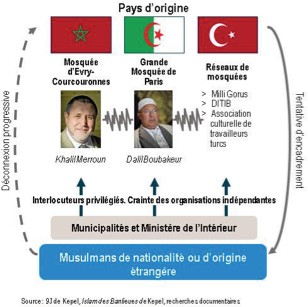
\includegraphics[width=\textwidth]{ImageIslamFrance/media/image7.jpeg}

\begin{enumerate}
\def\labelenumi{\arabic{enumi}.}
\item
  \textbf{Algérie : un acteur historique}
\end{enumerate}


Environ la moitié des ressortissants algériens qui vivent à l'étranger
résident en France. On estime qu'environ 1,5 million des musulmans de
France sont algériens ou d'origine algérienne, ce qui en fait la
communauté la plus importante numériquement parmi les musulmans de
France42. Cette importance démographique, ainsi que les liens
historiques qui unissent l'Algérie et la France, sont à l'origine de
cette volonté partagée par les deux pays de faire jouer à l'Algérie un
rôle majeur dans la gestion de l'islam en France.

L'islam consulaire algérien est apparu tardivement. En effet, dans les
années 1960 et 1970, l'Amicale des Algériens en Europe sert
principalement de \emph{« courroie de transmission entre un pouvoir
auréolé d'une indépendance fraîchement acquise et des migrants démunis
des solidarités communautaires »} ou joue un rôle

« d'interface » entre les migrants et les consulats algériens ou avec
les autorités françaisesii 43. Son rôle religieux est marginal
puisqu'elle n'a organisé la venue que de neufs imams

42 Bernard Godard, Sylvie Taussig, \emph{Les musulmans en France,}
Paris, Laffont, 2007.

43 Abdelhafid Hammouche, \emph{Des amicales d'hier aux associations de
quartier d'aujourd'hui. Un essai de typologie,} in Hommes et migrations,
n° 1229, janvier-février 2001.

II. L'ISL AM FRANÇAIS : UNE ORGANISATION PAR LE HA UT

durant cette période, afin d'offrir une assistance spirituelle aux
Algériens émigrésiii 44. Ce n'est qu'en 1982, lorsqu'Alger reprend le
contrôle de la Grande Mosquée de Paris, que l'État algérien commence à
financer le culte musulman en France, constitue un réseau d'associations
cultuelles et construit des salles de prières.

L'accession de Cheikh Abbas au poste de recteur de la Grande Mosquée de
Paris (GMP) marque un double tournant, à la fois dans le rôle de
l'Algérie à l'égard de l'islam en France et dans celui dévolu à la
Grande Mosquée de Paris. En effet, à partir des années 1980, l'État
algérien tente de s'imposer comme le chef de file de l'islam en France.
Ce rôle sera conforté par l'action de Charles Pasqua au ministère de
l'Intérieur. Il tente d'organiser l'islam français autour de la Grande
Mosquée de Paris et du réseau associatif cultuel algérien, en octroyant
à celle-là le « monopole » de l'abattage rituel en France. La guerre
civile, la décennie noire du terrorisme du GIA et les attentats de 1995
à Paris commis par des islamistes algériens, intensifieront cette
relation entre le gouvernement français et le pouvoir algérien. La
gestion de l'islam par les réseaux algériens apparaît alors comme une
garantie face à la montée de l'islamisme politique en France, lui-même
essentiellement importé d'AlgérieIV.

Malgré l'importance du rôle dévolu à l'islam consulaire algérien par les
pouvoirs publics, les élections successives du CFCM ont montré la
relative faiblesse des réseaux algériens auprès des musulmans de France.
La fédération nationale de la Grande Mosquée de Paris, qui rassemble
l'ensemble des associations cultuelles d'obédience algérienne, est ainsi
la grande perdante des premières élections de 2003, face à l'UOIF et à
la Fédération des Marocains de France : la nomination de Dalil
Boubakeur, recteur de la Grande Mosquée, à la tête du CFCM n'est due
qu'à l'accord passé préalablement avec Nicolas Sarkozy. Cet échec
électoral met à jour le décalage entre l'influence supposée, et
entretenue par le pourvoir public français, et celle réelle et effective
auprès des musulmans de France. Son expression la plus manifeste réside
dans le retrait de la fédération algérienne des instances du CFCM en
2008, refusant les règles du jeu démocratique et affirmant sa
prééminence sur l'islam français avec pour seuls arguments ceux du
nombre et du poids historique, avant son retour en 2012 lors de la
réforme du CFCM.

On estime aujourd'hui que la Grande Mosquée de Paris est forte d'un
réseau d'environ 250 associations et lieux de prières et qu'elle
contrôle environ 150 imams (soit 10\% environ des imams en France), dont
la majorité sont salariés

44 Jonathan Laurence, \emph{The emancipation of Europe's Muslims. The
State's role in minority integration,} Princeton University Press, 2012.



par l'Algérie (120 imamsv)45. Durant le mois du Ramadan, la France
accueille également 299 psalmodieurs et récitateurs dans le cadre
d'accords bilatéraux passés notamment avec le Royaume du Maroc et
l'Algérie. La répartition exacte de cet effectif n'est pas connue
publiquement. Ils disposent d'un visa de court séjour expirant le jour
de la fin du Ramadan et sont salariés par l'État émetteurvi 46. Malgré
un discours volontariste en matière d'accompagnement et d'encadrement de
l'islam français, notamment par sa participation à la formation des
cadres religieux aussi bien au sein de l'Institut Al-Ghazali implanté au
sein de la Grande Mosquée qu'au sein de l`université de Constantine,
l'État algérien demeure relativement en retrait. Ainsi ne participe-t-il
plus au financement du culte musulman en France qu'à hauteur de deux
millions d'euros par an environ, contre quatre millions en 2011, et près
de six millions pour le Marocvii 47. Comme le souligne Bernard Godard,
malgré sa puissance symbolique, la Grande Mosquée de Paris joue un rôle
marginal dans l'islam français : \emph{« sa construction même, puis sa
gestion, en ont fait un lieu diplomatique et officiel, mais nullement un
pôle intellectuel ou proprement religieux, en dépit de la présence d'un
``Institut musulman'' »}viii 48\emph{.}


\begin{enumerate}
\def\labelenumi{\arabic{enumi}.}
\setcounter{enumi}{1}
\item
  \textbf{Le Maroc : la puissance du Rassemblement des Marocains de
  France (RMF)}
\end{enumerate}


Environ un tiers des Marocains émigrés résident en France. Ils
constituent, derrière l'Algérie et son million et demi de
ressortissants, la seconde communauté musulmane française avec environ
un million de ressortissants (nationaux et binationaux)ix. Le Maroc
s'attache à maintenir un lien avec ses ressortissants, surtout depuis
les années 1980 et 1990. Cette politique poursuit deux objectifs : l'un
économique, lié à l'importance des remises migratoiresx ; l'autre
sécuritaire, lié à la lutte contre l'influence de l'islamisme politique
et terroriste.

À partir des années 1960, avec l'arrivée des premières vagues de
travailleurs immigrés marocains en France, l'État chérifien a mis en
place un réseau de contrôle relativement souple, avec notamment
l'Amicale des travailleurs et commerçants marocains en France (ATCMF).
La dimension économique est ici primordiale, car la communauté marocaine
s'est structurée religieusement sans véritable appui consulaire. Les
appels répétés du roi Hassan II aux Marocains à ne pas rompre le lien
les reliant au Maroc

45 Sénat, \emph{De l'Islam en France à un Islam de France, établir la
transparence et lever les ambiguïtés,} Rapport d'information établi par
Nathalie Goulet et M. André Reichardt n°757 (2015-2016), 5 juillet 2016.

46 Réponse apportée par M. le ministre de l'Intérieur Bernard Cazeneuve
à une question d'actualité au gouvernement n° 0747G de Mme Nathalie
Goulet, publiée au \emph{JO} Sénat du 12 février 2016.

47 Sénat, \emph{De l'Islam en France à un Islam de France, établir la
transparence et lever les ambiguïtés,} Rapport d'information établi par
Nathalie Goulet et M. André Reichardt n° 757 (2015-2016), 5 juillet
2016.

48 Bernard Godard, « Les états musulmans et l'Islam de France »,
Politique étrangère, 2015/3.

II. L'ISL AM FRANÇAIS : UNE ORGANISATION PAR LE HA UT

et à refuser l'abandon de la nationalité marocaine participent de à
cette volonté de maintenir l'effet diasporique.

Ce n'est que dans un second temps, sous l'effet de la montée de
l'islamisme au Maroc et en Europe, que le Royaume du Maroc met en place
une structure de contrôle religieux. L'État marocain va ainsi tenter de
rassembler les diverses associations musulmanes marocaines dans la
Fédération nationale des Marocains de France (FNMF), transformée depuis
en Rassemblement des Marocains de France (RMF). Depuis sa création, en
1990, la Fondation Hassan II a pour but, en étroite coordination avec le
ministère des Marocains résidant à l'étranger et le ministère des
Affaires religieuses, de diffuser la culture marocaine. Forte d'un
budget annuel de 15 à 20 millions de dollars, cette organisation envoie
des imams en Europe et finance les associations cultuelles marocaines.
Dans son récent rapport relatif à l'islam en France, le Sénat estime que
le Maroc salarie actuellement 30 imams détachés49. À l'occasion du
Ramadan, l'État chérifien \emph{« délègue également plus de 220 imams
par l'intermédiaire de la fondation Hassan II pour les Marocains
résidant à l'étranger »}xii 50, dont une partie en France.

Cette implication du Royaume chérifien dans la vie religieuse de ses
ressortissants est particulièrement prégnante si l'on considère le CFCM.
Par l'implantation majoritairement régionale des fidèles musulmans
d'origine marocaine et l'existence d'un réseau de mosquées dont la
surface est plus importante que celle des mosquées urbaines, la FNMF
remporte les premières élections du CFCM en 2003 ; elle devient la
principale bénéficiaire du mode de scrutin fondé sur la surface des
mosquées. Ce score fait prendre conscience aux autorités marocaines du
rôle déterminant qu'elles peuvent jouer dans l'islam français. Afin de
renforcer son poids dans l'instance représentative, le royaume du Maroc
fond la FNMF en une seule structure destinée à embrasser plus largement
encore l'ensemble des sensibilités des Marocains de France : le
Rassemblement des marocains de France (RMF).Cette politique volontariste
est un succès, comme le montrent les élections suivantes, que les
Français d'origine marocaine remportent largement en faisant ainsi
reculer l'UOIF. Au terme de son mandat, en 2008, Dalil Boukakeur,
recteur de la Grande Mosquée de Paris, sera ainsi remplacé par le
franco-marocain Mohammed Moussaoui.

L'implication de ressortissants d'origine marocaine dans les attentats
de Madrid en 2004 ainsi que la multiplication des actes de terrorisme
islamiste au Maroc ont conduit

49 Sénat, \emph{De l'Islam en France à un Islam de France, op. cit.}

50 S. Exc. M. Chakib Benmoussa, ambassadeur du Royaume du Maroc en
France, audition au Sénat dans le cadre de la Mission d'information
relative à l'organisation de l'islam en France.



son gouvernement à mener une lutte intense contre l'islamisme et le
terrorisme. C'est une véritable stratégie de contre-discours modéré que
tente de développer le Maroc en Europe, et plus particulièrement en
France. Elle passe par un contrôle accru des imams marocains présents
dans l'Hexagone, un renforcement de la présence d'imams agréés par le
gouvernement marocain, comme en témoigne l'accord passé en 2008 entre le
ministère de l'Intérieur français et le ministère des Affaires
religieuses marocains, prévoyant l'envoi de 30 imams en France, ou la
mise en place d'une offre de formation pour les apprentis-imams. Cette
politique d'encadrement religieux se double d'une politique de
financement : le Maroc participe ainsi au financement de la Grande
Mosquée de Strasbourg et finance en totalité la mosquée de
Saint-Étienne.

Au niveau européen, le Royaume chérifien crée, en 2010, un Conseil
européen des oulémas marocains, qui siège à Bruxelles. Selon Bernard
Godard, \emph{« Rabat tente d'installer en Europe une sorte de
contre-structure face à l'hyperactivité des deux ennemis principaux de
la conception chérifienne de la doctrine religieuse. Composé de
théologiens dont tous ne sont pas, loin s'en faut, des progressistes, il
doit contrebalancer une structure mise en place plus d'une décennie
auparavant par les Frères musulmans -- le Conseil européen de la fatwa
et de la recherche basé à Dublin --, mais doit aussi combattre la montée
inquiétante du salafisme qui influence les nouvelles générations en
Europe comme au Maroc}xiii 51\emph{»}

L'implication de ressortissants belges et français, dont certains
étaient d'origine marocaine, dans les attentats de novembre 2015 en
France ainsi que dans celui de Bruxelles en mars 2016 incitent l'État
marocain à poursuivre sa politique religieuse afin de se prémunir de la
contamination djihadiste qui peut venir d'Europe.

L'inauguration en 2015 de l'Institut Mohammed VI à Rabat, participe
pleinement de cette dynamique de rayonnement religieux : cette
structure, accueillant des apprentis imams du Maroc, mais aussi
d'Afrique et d'Europe, a pour mission d'« \emph{enseigner aux nouvelles
générations d'imams et de mourchidates} {[}prédicatrices{]} \emph{les
valeurs de l'islam du juste milieu en vue de prémunir le Maroc contre
les velléités de l'extrémisme »} et d'assurer « la sécurité spirituelle
du Maroc52 » et par extension de la France .

51 Bernard Godard, \emph{Les Etats musulmans et l'Islam de France, op.
cit.}

52 Discours du roi du Maroc lors de l'inauguration de l'Institut
Mohammed VI à Rabat, le 27 mars 2015, cité par Ruth Grosrichard dans
\emph{Le Monde.}

II. L'ISL AM FRANÇAIS : UNE ORGANISATION PAR LE HA UT


\begin{enumerate}
\def\labelenumi{\arabic{enumi}.}
\setcounter{enumi}{2}
\item
  
  \textbf{La Turquie : une gestion centralisée}
  
\end{enumerate}


Selon les informations fournies par les consulats turcs en France, il y
aurait environ 600 000 Turcs et Français d'origine turque en France. Ils
sont principalement présents dans l'est de la France, à proximité de
l'Allemagne, principal foyer d'émigration turque, et dans le sillon
rhodanien. Si l'État turc ne s'est guère préoccupé de ses populations
immigrées avant les années 1980, il accorde un intérêt croissant au
renforcement des liens avec sa diaspora et du contrôle religieux qu'il
exerce sur elle.

Aussi, le ministère des Affaires religieuses, le Diyanet, en
collaboration avec le ministère des Affaires étrangères et le ministère
des Turcs en émigration, a mis en place l'Union turco-islamique des
Affaires religieuses (la DITIB) qu'il administre et finance. La DITIB
assure l'encadrement religieux des populations turques émigrées. Partout
où vit une minorité turque immigrée en Europe, la DITIB prend en charge
les organisations culturelles et cultuelles turques existantes ou
nouvellement créées, et assure la prise en charge du pèlerinage à la
Mecque et du rapatriement des corps pour les enterrements en Turquie. On
estime ainsi que le ministère des Affaires étrangères à Ankara contrôle
et gère plus de cinq cents lieux de culte, sur les mille mosquées et
salles de prières turques recensées en Europe. La gestion de l'islam
consulaire turc est donc beaucoup plus centralisée que celle de
l'Algérie ou du Maroc. Il y a dans chaque consulat turc un représentant
du DITIB, qui est habilité à inspecter les mosquées turques affiliées et
à contrôler les imams qui y officient. Chaque imam détaché reçoit
régulièrement « un bulletin du Diyanet », contenant notamment les
prêches du vendredi élaborés par le pouvoir central. Actuellement 151
imams détachés par l'État turc officient à temps plein : cet effectif
représente la moitié des 301 imams détachés, envoyés par les pays
étrangers, et fait de l'État turc la puissance étrangère la plus
investie dans la gestion du culte musulman en Francexv 53.

Le mouvement du Millî Görüs, « Vision nationale » en turc, est le
principal concurrent du DITIB dans le contrôle religieux des émigrés
turcs. \emph{« Mélange de références proches de la mouvance des Frères
musulmans et d'exaltation de la grandeur perdue de l'Empire ottoman
»}54, le Millî Görüs rassemble de fervents opposants à la laïcité turque
et de farouches partisans du port du voile pour les jeunes fillesxvi 55.
Implanté en France dès l'arrivée des premiers Turcs, il est à l'origine
de la construction des premières mosquées turques. Son ancrage local et
sa présence historique lui permettent de s'appuyer sur une

53 Sénat, \emph{De l'Islam en France à un Islam de France, op.cit.}

54 Bernard Godard, « Les États musulmans et l'Islam de France »,
\emph{Politique étrangère,} 2015/3.

55 Bernard Godard, Sylvie Taussig, \emph{Les musulmans en France,}
Paris, Pluriel, 2009, p. 52.



organisation très structurée, qui dispose notamment d'une société
immobilière gérant l'ensemble de son patrimoine, et qui dispose de son
propre pavillon en Arabie Saoudite ; ce qui lui permet d'organiser le
pèlerinage.

Depuis sa création au milieu en 1984, le Diyan a renforcé son
implantation au sein de la communauté turque. La France compte
aujourd'hui trois fédérations DITIB, une à Paris, une à Lyon et une
dernière, créée en 1997 à Strasbourg, qui gère l'islam truc dans le
Grand-Est. Cette fédération strasbourgeoise, dotée d'un budget annuel de
500 000 e en moyenne et contrôlant une soixantaine de mosquées, est
devenue en quelques années un acteur majeur de l'islam régional. \emph{«
Longtemps la DITIB est restée cantonnée aux zones rurales et aux villes
moyennes d'Alsace, tandis que Strasbourg était le terrain du Millî Görüs
côté turc (Mosquée Eyyub Sultan de la Meinau) et du Rassemblement des
musulmans de France côté marocain »}xvii 56. L'accession d'un membre du
DITIB strasbourgeois à la présidence du CRCM ainsi que le développement
de projets éducatifs ambitieux (projet avorté de création d'une
université islamique et ouverture du lycée privé Yunus Emre à Strasbourg
en octobre 2015) constituent les éléments les plus visibles de cette
implantation : \emph{« Les courants islamiques turcs d'Europe ont
développé un islam social extrêmement actif. Focalisées sur le
resserrement des liens communautaires, leurs actions se développent sur
trois axes: création de mosquées, enseignement avec une réaffirmation de
valeurs traditionnalistes teintées d'ottomanisme et entraide sociale et
scolaire »}xviii 57.


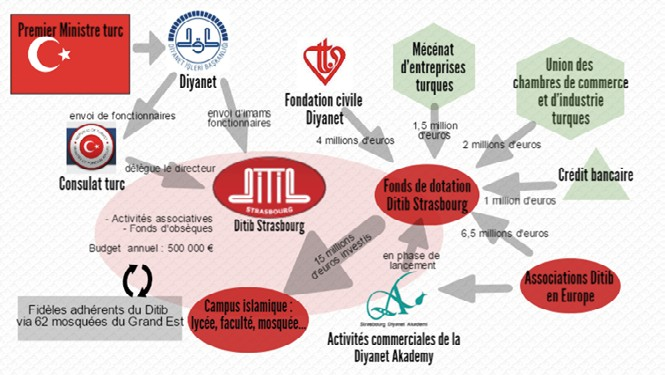
\includegraphics[width=\textwidth]{ImageIslamFrance/media/image8.jpeg}


Source : Claire Gandanger, sur
\href{http://www.rue89strasbourg.com/}{www.rue89strasbourg.com.}

56 Claire Gandanger, « Ditib : la montée en puissance de l'islam
officiel turc à Strasbourg », \emph{rue89}, 2 octobre 2015.

57 Samin Akgönul, « Islam turc, islams de Turquie : acteurs et réseaux
en Europe », \emph{Politique étrangère,} 2005/1.

II. L'ISL AM FRANÇAIS : UNE ORGANISATION PAR LE HA UT

L'islam turc ne vise pas à être hégémonique en France, mais à entretenir
l'adhésion des musulmans d'origine turque à la Turquie. Cet encadrement
très structuré, qui nourrit une vie et une pratique communautaires,
constitue à la fois un frein à l'intégration des Turcs en France mais
aussi à la propagation du salafisme parmi la communauté musulmane
d'origine turquexx 58.

La Tunisie est la grande absente de ce tableau des interactions entre
les pays du Maghreb et l'islam. Pourtant, à la fin des années 1980, les
premiers dirigeants de l'UOIF étaient des Tunisiens, chassés de Tunisie
par Bourguiba et Ben Ali. L'État tunisien, sous Ben Ali, utilisait
davantage le contrôle sécuritaire et policier des individus que la
gestion via l'islam et les mosquées des populations immigrées
tunisiennes en France (et en Europe). La Tunisie n'apparaît donc pas
comme un acteur majeur de l'islam en France.


Le financement étranger de l'islam en France


Dans son rapport sur le financement des lieux de culte, conduit en 2015
sous la direction du sénateur Pierre Maurey, le Sénat souligne que :


\begin{itemize}
\item
  le financement du culte dans son ensemble (dépenses de fonctionnement
  et dépenses d'investissement) est assuré majoritairement par les
  fidèles eux- mêmes. La \emph{zâkat}, équivalent musulman du denier du
  culte chez les catholiques, contribue à un relatif autofinancement du
  culte ;
\item
  
  les États étrangers et les organisations transnationales participent
  également au financement du culte musulman français, mais de façon
  marginale. Ce financement exogène sert notamment d'aide à la
  construction de lieux de cultes ou à leur entretien, et également au
  salariat des imams détachés par certains pays.
  
\end{itemize}


Les auditions des ambassadeurs de l'État algérien et du royaume du Maroc
ont mis en valeur la relative faiblesse du financement issu des États
étrangers.

L'Algérie ne participe qu'indirectement au financement du culte musulman
en France. Ce financement prend la forme d'une subvention globale versée
à la Grande Mosquée de Paris, qui en affecte ensuite une partie à son
propre fonctionnement et l'autre aux associations, mosquées et salles de
prières membres de la Fédération nationale de la Grande Mosquée de Paris
qui en formulent expressément la demande. L'aide financière algérienne à
destination de la communauté musulmane française est en

58 Mohammed-Ali Adraoui, \emph{Du golfe aux banlieues : le salafisme
mondialisé,} Paris, PUF, 2013.



diminution. Si, en 2011, elle était de quatre millions d'euros environ,
en 2013, elle n'est plus que de 1,8 million. Les montants affectés aux
associations et mosquées qui en font la demande varient entre 20 000 et
49 000 euros par projet.

L'aide marocaine est, elle, en augmentation. De quatre millions d'euros
en 2013, elle s'élève à six millions d'euros en 201659. Ce financement
est direct et obéit à une procédure stricte : \emph{« les demandes de
financements adressées au Maroc émanent toujours d'associations de
fidèles et transitent par l'ambassade ou sont déposées directement
auprès du ministère marocain des Affaires religieuses »}60.

L'aide marocaine en 2013 est répartie comme suit :


\begin{itemize}
\item
  « Un tiers » des fonds a été affecté à la construction et à la
  rénovation de mosquées (Saint-Étienne, Strasbourg, Blois, Évry et
  Mantes-la-Jolie) ;
\item
  « Un autre tiers » a été dirigé vers des associations cultuelles ;
\item
  
  « Le dernier tiers » sert à financer le salaire des imams et
  prédicateurs qui viennent temporairement en France durant le mois de
  ramadan, qui se caractérise par une fréquentation accrue des mosquées.
  
\end{itemize}


Ces données révèlent l'existence d'une demande réelle de financement du
culte par les États étrangers de la part des associations cultuelles et
des mosquées. Toutefois, cette demande reste marginale, et relativement
transparente.

En revanche, il existe une véritable opacité autour des dons privés
étrangers, qui participent également au financement du culte musulman,
ainsi que le souligne le Sénat dans son rapport sur l'Islam en France :
\emph{« À l'instar des dons privés de source française, ces dons privés
étrangers, éclatés, ne peuvent faire l'objet d'une collecte statistique
exhaustive. Ils sont pourtant, sans nul doute, ceux qui suscitent, dans
l'opinion publique, le plus de suspicion, quant à l'orientation
idéologique qui les anime61. »}

Le fait que la majorité des associations musulmanes soient de type « loi
de 1901 » et non des associations cultuelles telles que les définit la
loi de 1905 participe de

59 Sénat, « De l'Islam en France à un Islam de France, établir la
transparence et lever les ambiguïtés », \emph{Rapport d'information}
établi par Nathalie Goulet et M. André Reichardt, n°757 (2015-2016), 5
juillet 2016.

60 Audition de l'ambassadeur du Maroc, M. Chakib Benmoussa, cité dans
Sénat, « Les collectivités territoriales et le financement des lieux de
culte », Rapport d'information, 2015.

61 Sénat, « De l'Islam en France à un Islam de France, établir la
transparence et lever les ambiguïtés », \emph{Rapport d'information}
établi par Nathalie Goulet et M. André Reichardt, n°757 (2015-2016), 5
juillet 2016, p.60.

II. L'ISL AM FRANÇAIS : UNE ORGANISATION PAR LE HA UT


\hypertarget{les-pays-uxe9trangers-uxe9metteurs-diduxe9ologie-rigoriste}{%
\subparagraph{Les pays étrangers émetteurs d'idéologie
rigoriste}\label{les-pays-uxe9trangers-uxe9metteurs-diduxe9ologie-rigoriste}}


\textbf{L'Arabie Saoudite et le wahhabisme : la religion comme soft
power}

Bien que l'Arabie Saoudite ne soit pas un pays exportateur de
main-d'œuvre en Europe, l'État saoudien a de longue date cherché à
étendre l'influence religieuse du Royaume dans les pays européens. Ses
réserves pétrolières lui donnent une solide assise financière, qui lui
permet d'être un acteur majeur dans le champ religieux musulman, comme
dans le champ politique européen. La diffusion de l'islam wahhabite est
ainsi étroitement liée aux objectifs politiques du Royaume. L'islam
wahhabite a donc été un instrument de politique étrangère utilisé,
durant les années 1960 et 1970, pour lutter contre l'influence du
nationalisme arabe porté par l'Égypte nassérienne notamment. Depuis les
années 1980, face à l'émergence de la République Islamique d'Iran,
l'Arabie Saoudite s'est engagée dans une lutte pour \emph{« contrôler
l'espace de sens islamique du monde musulman »62.}

L'expansion internationale des activités religieuses de l'Arabie
Saoudite s'inscrit dans une période clef des relations entre les
sociétés de langue arabe et les pays européens, qui correspond également
à la période où l'immigration musulmane s'implante durablement en
Europe. Le soutien américain à la Guerre de Kippour en 1973 et l'embargo
pétrolier \underline{de l'Organisation des pays exportateurs de pétrole
(OPEP) qui en résulte font de l'Arabie}

62 Zak iLaïdi, \emph{Géopolitique du sens,} Paris, Desclée de Brouwer,
1998.



Saoudite -- détentrice de près de 22 \% des réserves pétrolières
mondiales -- un acteur déterminant des relations entre l'Occident et le
Moyen-Orient. C'est cette inversion de la relation de pouvoir entre le
monde arabe et l'Ouest qui permet à l'Arabie Saoudite de se constituer
en véritable \emph{« superpuissance religieuse »}63\emph{.}

Ainsi, en 1962, à La Mecque, a été fondée la Ligue islamique mondiale --
LIM \emph{(Rabitat al-Alamiyya al-Islamiyya)}, sous l'impulsion du
prince Fayçal Ibn Abdel Aziz. Véritable relais d'influence de la
diplomatie culturelle et religieuse saoudienne, cette organisation
remplit deux missions principales : elle diffuse l'idéologie
panislamique face à l'émergence des nationalismes arabes et elle vise à
assurer l'hégémonie de l'Arabie Saoudite sur l'islam mondial. Structurée
en plusieurs départements, la Ligue islamique mondiale gère la formation
des imams, distribue des bourses aux étudiants et lutte contre le
christianisme. Elle dispose aujourd'hui de 120 antennes réparties dans
le monde entier et de plusieurs institutions subsidiaires telles que le
Conseil islamique européen, à Londres. Dirigé par un Frère musulman
égyptien, qui a trouvé asile en Arabie Saoudite, le Conseil islamique
européen joue un rôle important dans le rapprochement des organisations
musulmanes européennes et de la Ligue islamique mondiale. La Ligue a un
centre dans chaque capitale européenne : celui de Paris a ouvert en
1977.

Cette Ligue joue un rôle de mécénat très important. La puissance
financière de l'Arabie Saoudite a permis à la Ligue islamique mondiale
de devenir un acteur majeur dans la mise en place des infrastructures
cultuelles musulmanes en Europe. Ce sont des centaines de millions de
dollars qui ont été dépensés dans la construction de mosquées dans toute
l'Europe : France, Espagne, Italie, Pays-Bas, Belgique, Royaume-Uni,
etc. En France, l'Arabie Saoudite a notamment participé au financement
de la construction de la mosquée de Mantes-la-Jolie en 1980, de celle
d'Évry en 1984 et de celle de Lyon en 1994 -- que le prince Fahd est
venu inaugurer en personne, après avoir fait un don de quatre millions
de dollars. La LIM pourrait avoir dépensé environ 40 millions de dollars
dans la construction de mosquées en France et dans le financement
d'associations cultuelles. \emph{« Par ces différentes aides
financières, il ne s'agissait pas tant d'infléchir l'islam de France
dans un sens wahhabite que d'asseoir une forme d'autorité financière et
matérielle auprès des populations musulmanes de France, en constituant
des réseaux d'allégeances et de clientèle »64.} L'Arabie Saoudite
continue, par ailleurs, à financer des actions sociales et caritatives,
sans qu'il soit possible de mesurer précisément les flux financiers
engagés.

63 Samir Amghar, « Acteurs internationaux et islam de France », \emph{in
Politique Etrangère}, 2005/1.

64 SamirAmghar, « Acteurs internationaux et islam de France »,
\emph{Politique étrangère} 2005/1 (Printemps), p. 30.

II. L'ISL AM FRANÇAIS : UNE ORGANISATION PAR LE HA UT

Au-delà du développement d'un réseau d'influence international au
travers de la LIM, l'Arabie Saoudite a réussi à se constituer un
véritable pôle d'influence de rayonnement religieux. Cette stratégie a
pris deux directions.

L'Arabie Saoudite a considérablement développé les moyens d'accueil des
pèlerins lors du \emph{hajj}. Fort de deux lieux saints de l'islam, La
Mecque et Médine, le Royaume saoudien est devenu un haut lieu de
pèlerinage mondial : chaque année, près de six millions de pèlerins se
rendent à La Mecque (ils sont près de deux millions à faire le
\emph{hajj} alors qu'ils n'étaient que 150 000 dans les années 1950), où
leur sont distribués gratuitement des livres de littérature islamique
wahhabite. En France, ils sont 25 000 à effectuer le \emph{hajj} chaque
année. Environ 5 \% des musulmans français se sont rendus au moins une
fois à La Mecque tandis que près de 75 \% de personnes qui se déclarent
musulmanes envisagent de s'y rendre au cours de leur vie.

Le second axe de cette stratégie d'influence religieuse consiste à
développer d'importantes universités islamiques à La Mecque (université
al-Mukkarama), à Médine (université al-Munawwara) ou à Riad (université
Ibn Saûd), afin de concurrencer directement les grandes universités
historiques comme celle d'Al-Azhar en Égypte, de la Zaytouna en Tunisie
ou d'Al Karawiyineau Maroc. L'État saoudien a ainsi mis en place de
nombreuses bourses d'études afin d'accueillir des étudiants en théologie
du monde entier souhaitant devenir imams. Une fois de retour dans leur
pays, ceux-ci deviennent de véritables ambassadeurs et constituent un
important vecteur de propagation du wahhabisme.

L'expansion fulgurante de l'influence saoudienne, grâce à la
construction de grandes mosquées, à la distribution gratuite de millions
de livres ou de brochures wahhabites et à la formation d'imams, s'appuie
sur la manne financière que constituent les réserves pétrolières. Selon
James Wolsey, cette politique d'influence et de rayonnement religieux
aurait mobilisé plus de 85 milliards de dollars entre 1975 et 2005 au
niveau mondial65 et viserait une hégémonie spirituelle et politique sur
la pratique musulmane66.

Cette politique de rayonnement religieux s'appuie essentiellement sur
des intermédiaires et se caractérise par une faible présence physique
sur le terrain. L'ambassadeur du royaume d'Arabie Saoudite en France,
Khalid bin Mohammed Al Ankary, a ainsi indiqué que l'État saoudien,
depuis 2011, \emph{« avait participé au financement de huit mosquées
\underline{françaises : les aides ont varié entre 200 000 et 900 000
euros par projet. Au}}

65 Shehabi, « The role of religious ideology in the expansionist
policies of Saudi Arabia », in Madawi Al-Rasheed, \emph{Kingdom without
Borders, Saudi Political, religious and Media Frontiers,} New-York,
Columbia University Press, 2008, p. 183-197.

66 James Woolsey, « The Global Spread of Wahhabi Islam : How Great a
Threat ? », Pew Forum on Religion and Public Life, 3 mai 2005.



\emph{total, nous avons versé 3 759 400 euros »}67\emph{, soit en
moyenne 750 000 euros par an.} Il a également précisé que l'Arabie
Saoudite ne finance le salaire que de 14 imams sur les quelque 2 200 qui
officient en France.




\begin{figure}
    \centering
    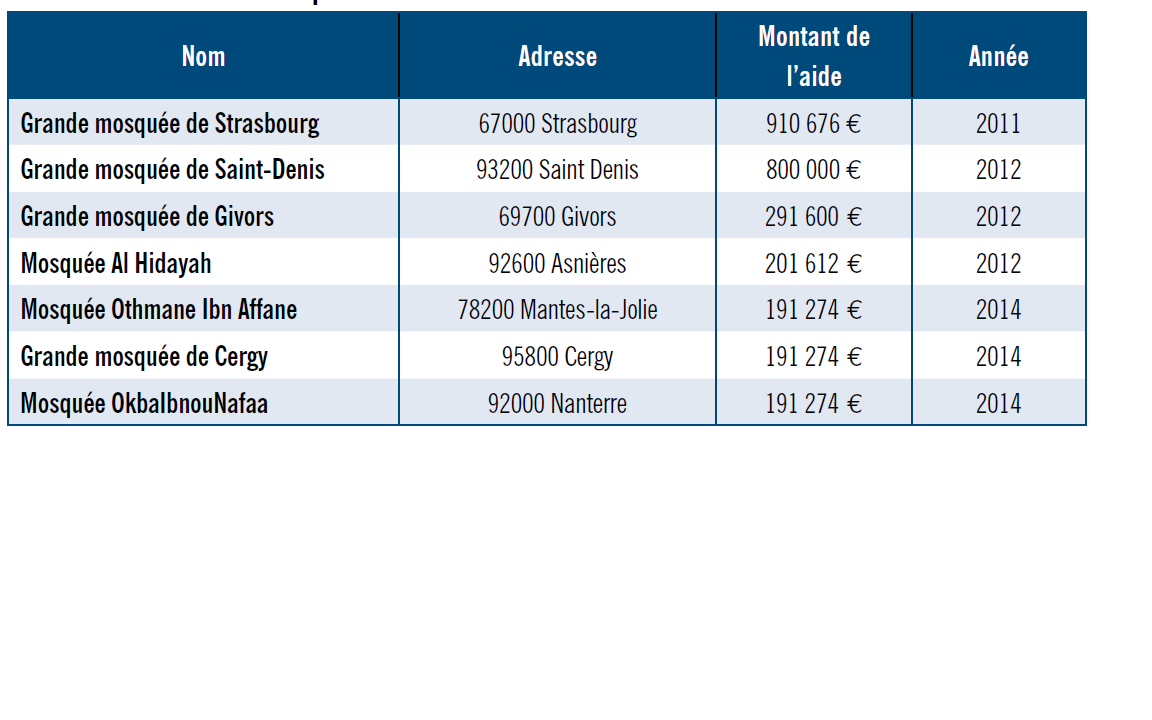
\includegraphics[width=\textwidth]{ImageIslamFrance/MosqueeArabieSaoudite.png}
    \caption{Liste des mosquées situées en France dont l'Arabie saoudite a
partiellement financé la construction68}
    \label{fig:MosqueeArabieSaoudite}
\end{figure}

\textbf{Le Qatar : la puissance financière et cathodique au service
d'une stratégie oblique}

Le Qatar opère davantage sur le paysage de l'islam français selon une
logique financière clientéliste et logistique que \emph{via} les
vecteurs traditionnels de l'islam consulaire. Et ce, en s'appuyant sur
des vecteurs médiatiques, déterritorialisés, tels que Tariq Ramadan69,
ou « d'imams cathodiques » tels que le cheikh Youssef. Al-Qaradhâwî,
architecte de l'exportation télévisuelle de la vision islamiste qatarie,
qui \emph{via} l'émission « La charia et la vie » \emph{(al-sharî `a wa
al-hayât),} produite par la chaîne Al-Jazira, s'adresse directement aux
musulmans français maîtrisant l'arabe classique.

67 Sénat, Rapport d'information n° 757 sur l'organisation, la place et
le financement de l'Islam en France et de ses lieux de culte, juillet
2016.

68 Sénat, « De l'Islam en France à un Islam de France, établir la
transparence et lever les ambiguïtés », Rapport d'information établi par
Nathalie Goulet et M. André Reichardt, n° 757 (2015-2016), 5 juillet
2016

69 Directeur du \emph{Centre de recherche pour la législation islamique
et l'éthique} (CILE), inauguré à Doha, le 15 janvier 2012 et professeur
en études islamiques contemporaines à St Anthony's College (Oxford), sur
une chaire au nom de l'ancien émir du Qatar : HH Sheikh Hamad Bin
Khalifa Al-Thani.

II. L'ISL AM FRANÇAIS : UNE ORGANISATION PAR LE HA UT

Selon Haoues Senigher70, les mécènes qataris font \emph{« régulièrement
des dons à l'Union des Organisations Islamiques de France (UOIF),
héritière, et caisse de résonance française, de l'idéologie des Frères
musulmans que partage précisément une majorité d'officiels qataris. »}


\hypertarget{luoif-un-islam-uxe0-la-franuxe7aise}{%
\paragraph{L'UOIF: UN ISLAM À LA FRANÇAISE
?}\label{luoif-un-islam-uxe0-la-franuxe7aise}}

\hypertarget{origines-et-organisation}{%
\subparagraph{Origines et organisation}\label{origines-et-organisation}}


L'Union des organisations islamiques de France (UOIF) est une composante
importante du paysage de l'islam français. Fondée en 1983 par des
étudiants tunisiens en exil, proches du Mouvement de la tendance
islamique (MTI), l'ancêtre d'Ennahda, fuyant la répression du président
Bourguiba, avait pour objectif initial de fonder une branche française
du parti islamiste tunisien. Historiquement proche des Frères musulmans,
dont elle constitue un acteur majeur de la branche européenne, l'UOIF,
lors de sa création, tenait un discours islamiste. Conformément à la
doctrine élaborée par Hassan Al-Banna, le fondateur du mouvement des
Frères Musulmans en 1927, les fondateurs de l'UOIF affirmaient que
l'islam est un système complet, qui concerne tous les aspects de la
vie71 ; il n'est donc pas seulement religieux, mais aussi politique et
social. L'objectif recherché par les Frères Musulmans est l'avènement
d'une société islamique régie par la charia.

Si ce discours islamiste est encore présent au sein de l'UOIF,
l'institutionnalisation de cette organisation, notamment à l'occasion de
la création du CFCM en 2003, a contribué à faire évoluer son discours et
à le conformer aux valeurs démocratiques occidentales. Aujourd'hui,
l'UOIF est une fédération qui regroupe environ \emph{« 250 associations
musulmanes réparties sur tout le territoire français »}72, mais aussi le
cadre d'accueil d'une multitude de discours dont le degré d'islamisme
est variable -- puisqu'elle invite aussi bien Tareq Oubrou, qui récuse
par exemple le port du voile, qu'Amar Lasfar, l'actuel président, qui
défend des positions bien plus conservatrices. La pluralité des
discours, ainsi que leur éventuelle contradiction sont le reflet des
mutations profondes

70 Séniguer Haoues, « Le Qatar et l'islam de France : vers une nouvelle
idylle ? », \emph{Confluences Méditerranée,} 1/2013 (n° 84), p. 101-115

71 Premier principe d'Hassan Al-Banna.

72 Présentation de la fédération sur son site internet, consulté le 18
août 2016
\href{http://www.uoif-online.com/presentation/)}{(http://www.uoif-online.com/presentation/).}



qui se sont opérées au sein de la communauté musulmane en France et
l'expression des tensions qui traversent cette organisation, entre
inscription dans un réseau transnational et rôle majeur dans l'émergence
de l'islam français.

Cette hétérogénéité des logiques à l'œuvre se retrouve dans la
composition de son budget de fonctionnement, estimé à plus de deux
millions d'euros annuels. Samir Amghar note en effet que 60 \% de son
financement serait issu de ses recettes propres (cotisations des
associations membres, recettes liées aux bénéfices de sa branche
commerciale -- l'association GEDIS, à la fois maison d'édition et
principal organisateur du forum annuel de l'UOIF au Bourget), tandis que
40 \% proviendraient de dons de mécènes du Golfe ou de subventions d'ONG
proches de l'Arabie Saoudite73. La part importante des financements
internationaux dans le fonctionnement de l'UOIF est due à son
inscription dans le réseau transnational que constitue la mouvance des
Frères musulmans. Ce réseau lui permet ainsi de bénéficier de
financements provenant de pays du Golfe et notamment de l'Arabie
Saoudite, qui servit de refuge aux principaux responsables des Frères
musulmans après l'interdiction de ce mouvement en Égypte par Nasser en
195474.

L'UOIF est membre de la FOIE (Fédération des organisations islamiques
européennes -- FIOE en anglais), organisation cofondée en 1989 avec
d'autres fédérations nationales européennes -- elles aussi affiliées aux
Frères musulmans -- telles que \emph{l'Islamitische Gemeinschaft in
Deutschland,} en Allemagne, la \emph{Muslim Association of Britain}
(MAB) en Angleterre, la Ligue Islamique interculturelle de Belgique
(LIIB), la Ligue des musulmans de Suisse (LMS 1992) et l'\emph{Unione
delle Communita e delle Organizazioni Islamiche in Italia} (UCOII 1990).
L'UOIF a ainsi joué un rôle majeur dans la création du Conseil européen
de la Fatwa et de la Recherche (CEFR), fondé en 1997. Cette institution
a la charge d'élaborer une jurisprudence adaptée au contexte européen et
de rendre des avis juridiques.

L'UOIF est ainsi une organisation mise en tension entre une logique de
développement transnational et une opportunité de participer à la
définition d'un islam français. Elle doit concilier plusieurs échelles
de développement, allant du niveau local au niveau international.

73 Samir Amghar, « Les mutations de l'islamisme en France. Portrait de
l'UOIF, porte-parole de l'\,``islamisme de minorité'' »,

\emph{La Vie des idées,} 1er octobre 2007.

74 Stéphane Lacroix, \emph{Les islamistes saoudiens. Une insurrection
manquée,} Paris, Presses universitaires de France, 2010.

II. L'ISL AM FRANÇAIS : UNE ORGANISATION PAR LE HA UT

En effet, ce n'est pas uniquement son inscription dans des réseaux
transnationaux et européens qui donne à l'UOIF un rôle particulier au
sein du paysage musulman français, mais aussi son assise territoriale et
son dynamisme local. Comme le souligne Vincent Geisser : \emph{« sa
réussite doit moins à une planification centralisée -- un plan
d'islamisation défini préalablement par une ``technocratie islamique''
-- qu'à une synergie de succès locaux et sectoriels. (\ldots) En somme,
l'épopée de l'UOIF se fonde sur une synergie d'épopées locales75 ».}

La puissance de l'UOIF réside dans sa capacité à fédérer autour d'un
discours et d'une idéologie des dynamiques locales relativement
hétérogènes. Ainsi, à Bordeaux, les associations affiliées à l'UOIF sont
majoritairement issues du milieu étudiant, universitaire et
intellectuel, tandis que dans le Nord de la France, ce sont des
associations populaires, ouvrières et obéissant à des logiques
ethno-nationales. Cette stratégie de maillage territorial s'inspire de
l'organisation des partis politiques. L'UOIF a ainsi divisé le
territoire français en huit régions avec, à la tête de chacune, un
représentant de la fédération. En sus des quelques 250 associations qui
lui sont affiliées elle contrôle une trentaine de centres cultuels ainsi
que deux grandes mosquées -- Lille Sud dont le recteur est Amar Lasfar
-- actuel président de l'UOIF-- et Bordeaux, qui a pour imam Tareq
Oubrou.

En complément de cette fédération d'associations musulmanes s'ajoute une
stratégie de sectorisation de ses activités et de quadrillage de la
société islamique française76. Des Jeunes musulmans de France aux
Étudiants musulmans de France, de la Ligue française de la femme
musulmane à l'Association des imams de France, en passant par le milieu
médical avec l'association Avicenne, c'est une véritable segmentation de
la communauté musulmane française qui est opérée. \emph{« Chaque secteur
de la ``société musulmane'' est considéré comme une part de marché à
conquérir77 ».} Cela permet à l'UOIF d'engager un processus de
légitimation. La formulation d'un discours destiné à chaque segment,
parfaitement calibré, lui permet de se définir comme l'instance
représentative de ce segment.

Ce quadrillage de la vie islamique donne à l'UOIF un véritable avantage
comparatif, voire une place en situation de quasi monopole. C'est le cas
concernant la formation des imams. L'ouverture, dès 1991, de l'Institut
Européen des Sciences Humaines (IESH), près de Nevers, puis au début des
années 2000, d'une antenne à Saint-Denis, lui

75 Vincent Geisser, « L'UOIF, la tension clientéliste d'une grande
fédération islamique », in \emph{Confluences méditerranéennes,}

2006/2, n° 57, p. 83 à 101.

76 Samir Amghar, \emph{op. cit.}

77 Samir Amghar, \emph{op. cit.}



ont donné une véritable avance en la matière. Outre l'incapacité de
l'État à élaborer une structure de formation des cadres religieux
musulmans, cette situation quasi- monopolistique est renforcée par
l'intégration de l'UOIF dans un réseau transnational et européen. Ainsi,
les cadres religieux musulmans suisses sont-ils formés à l'IESH, suite à
un accord entre les autorités publiques helvétiques et l'institut
privé78.

Cette double stratégie de maillage territorial et de sectorisation de la
société islamique alimente un puissant processus de légitimation. La
double affirmation quasi-performative d'être l'institution la plus
représentative de l'islam de France, et d'être omniprésente dans le
champ islamique français, dont elle définit quasi-exclusivement le
périmètre, lui offre l'opportunité d'être l'un des principaux
interlocuteurs des pouvoirs publics en matière d'organisation de l'islam
français.


\hypertarget{un-acteur-de-lislam-de-france}{%
\subparagraph{Un acteur de l'islam de
France}\label{un-acteur-de-lislam-de-france}}


Ce désir de jouer un rôle déterminant dans l'organisation de l'islam en
France emprunte deux voies : l'affirmation d'une autonomie
organisationnelle à l'égard d'intérêts ethniques ou nationaux, d'une
part; un \emph{« travail de ``nationalisation'' de sa rhétorique
officielle »}79, d'autre part. Ainsi, l'UOIF affirme-t-elle
régulièrement son indépendance. Elle se présente comme une émanation de
la communauté musulmane de France, détachée de tout lien avec les États
d'origine ; et, partant, comme un acteur incontournable de
l'organisation d'un islam français. De même, le discours de
l'organisation accompagne les évolutions de l'islam français. Il est
remarquable que l'UOIF ait transformé son nom en 1989, l'Union des
organisations islamiques en France devenant l'Union des organisations
islamiques de France, marquant ainsi le passage d'un islam transitoire
et provisoire à un islam définitivement ancré dans le paysage français.
Ce changement de nom est d'ailleurs concomitant de l'événement qui
marque la naissance de l'UOIF sur la scène politique française et comme
acteur majeur de l'islam en France : l'affaire du voile de Creil (1989).
S'opère également à la même période un profond renouvellement des cadres
de l'organisation : en 1994, la « majorité tunisienne » qui dirigeait
jusqu'alors l'UOIF est écartée au profit d'une « majorité marocaine »,
dont les liens avec la mouvance des Frères musulmans sont moins marqués.

L'UOIF est ainsi progressivement devenue un interlocuteur incontournable
des pouvoirs publics. Le premier mouvement de reconnaissance
institutionnelle s'est opéré durant le

78 France Messner, « La formation des cadres religieux musulmans »,
Rapport, 2013.

79 Vincent Geisser, \emph{op. cit.}

II. L'ISL AM FRANÇAIS : UNE ORGANISATION PAR LE HA UT

second mandat de François Mitterrand, à l'occasion de la création de
l'éphémère CORIF (Conseil de réflexion sur l'islam en France) par Pierre
Joxe : l'UOIF siège alors parmi les 15 membres qui composent ce Conseil.
Il sera vite abandonné par Charles Pasqua qui préfère faire de la
mosquée de Paris, d'obédience algérienne, le principal acteur de
l'organisation de l'islam français. Cette brève expérience constitue
toutefois pour l'UOIF le début de \emph{« la lente marche vers
l'institutionnalisation »}80.

Le lancement en 1999 par Jean-Pierre Chevènement, alors ministre de
l'Intérieur, d'une \emph{« consultation des représentants des
principales sensibilités musulmanes sur l'organisation du culte
islamique en France »} dite « istichara », qui préfigure la création du
CFCM, marque une nouvelle étape dans le processus
d'institutionnalisation de l'UOIF. À cette occasion, elle se révèlera
être un acteur politique déterminant dans l'émergence d'un islam
français : tout au long du processus de création de l'instance
représentative qu'est amené à être le CFCM, les représentants de
l'association parviendront à faire prévaloir leurs vues concernant sa
mise en place et sa composition. Conformément aux exigences de l'UOIF,
l'organisation du CFCM sera décentralisée et les instances régionales
occuperont un rôle essentiel, aussi bien dans le fonctionnement de
l'organisation que dans la désignation des membres qui siègeront dans
l'instance nationale.

Néanmoins, c'est véritablement alors que Nicolas Sarkozy est ministre de
l'Intérieur que l'UOIF connaît sa consécration politique : entre le
Ministre et l'UOIF s'établissent d'étroites relations que Vincent
Geisser qualifie de \emph{« clientélisme consenti »} : « (\ldots)
\emph{le déploiement de la configuration clientéliste ``UOIF-Sarkozy''
peut se résumer à l'histoire d'une rencontre ``heureuse'' entre un
acteur communautaire (une fédération islamique) désireux d'obtenir une
reconnaissance institutionnelle rapide et un acteur politique
pragmatique (un ministre de l'Intérieur) à la recherche d'un
interlocuteur musulman ``crédible'' et relativement indépendant des
États étrangers. »}81. Cette reconnaissance mutuelle culminera avec la
présence de Nicolas Sarkozy au Bourget, en 2003, lors du rassemblement
annuel de l'UOIF82.

80 Bernard Godard, Sylvie Taussig, \emph{Les musulmans en France,}
Paris, Pluriel, 2009, p. 52.

81 V. Geisser, \emph{op.cit.} p. 93 et 94.

82 Thami Breze, président de l'UOIF alors, déclara à l'occasion de cette
visite, le 19 avril 2003 au Bourget : \emph{« Nous recevons un ami, que
nous avons découvert et qui nous a découverts ».}




\hypertarget{la-notabilisation-et-linstitutionnalisation-duxe9clin-ou-neutralisation-de-luoif}{%
\subparagraph{La notabilisation et l'institutionnalisation : déclin ou
neutralisation de l'UOIF
?}\label{la-notabilisation-et-linstitutionnalisation-duxe9clin-ou-neutralisation-de-luoif}}


Cette reconnaissance politique de l'UOIF n'est toutefois pas sans
conséquence sur celle-ci. Devenue un interlocuteur régulier des pouvoirs
publics et -- surtout à la suite de la première élection des
représentants du CFCM et des Conseils régionaux du culte musulman (CRCM)
-- l'un des principaux représentants des musulmans de France, en
obtenant 13 sièges sur 41 au Conseil d'administration ainsi qu'une
vice-présidence, l'UOIF doit, en retour, revoir à la baisse ses
revendications.

Son progressif ralliement aux institutions françaises, partant de sa
progressive institutionnalisation, se traduisent en effet par ses prises
de positions. C'est ainsi que l'UOIF, qui avait été à la pointe du
combat politique pour le port du voile dans les établissements
scolaires, appellera ses sympathisants à ne pas participer aux
manifestations de protestation contre la loi relative à l'interdiction
du port de signes ostentatoires à l'école. Dans un même souci de
légitimation auprès des pouvoirs publics, l'UOIF émettra une fatwa
appelant à la cessation des violences urbaines lors des émeutes de 2005.
Cette intervention n'ayant eu aucune incidence sur les émeutes, Gilles
Kepel y voit la marque d'une perte d'influence de l'UOIF auprès des
musulmans de France ; conséquence d'une trop grande
institutionnalisation de l'organisation et d'une relative

« notabilisation » de ses dirigeants qui les couperait du reste de la
communauté83.

Cette perte d'influence est renforcée par la crise du militantisme qui,
au cours des années 2000, touche l'ensemble des organisations,
fussent-elles politiques, syndicales ou associatives. Celle-ci est
d'autant plus marquée au sein de l'UOIF qu'elle s'accompagne d'un double
conflit, générationnel et social. En effet, le renouvellement des cadres
de l'organisation est difficile et révèle l'existence d'un fossé entre
des cadres originaires du Maghreb et des militants et sympathisants qui,
bien qu'issus de l'immigration, sont nés et ont grandi en France :
aujourd'hui encore, les principaux responsables de l'UOIF


\begin{itemize}
\item
  
  majoritairement originaires du Maghreb -- pratiquent une endogamie qui
  empêche l'accès aux responsabilités de musulmans français. De
  surcroît, le choix effectué au début des années 1990 de former la
  future élite musulmane française a conduit l'UOIF à privilégier le
  développement d'organisations telles que les Jeunes musulmans de
  France ou les Étudiants musulmans de France, afin de cibler un segment
  de population bénéficiant d'un niveau scolaire relativement élevé et
  engagé dans la poursuite d'études universitaires. Cette orientation
  s'est faite au détriment de jeunes musulmans vivant \underline{dans
  des quartiers difficiles, relativement exclus. La conjonction de la
  perte de radicalité}
  
\end{itemize}


83 Gilles Kepel, \emph{Quatre-vingt-treize,} Paris, Gallimard, 2012

II. L'ISL AM FRANÇAIS : UNE ORGANISATION PAR LE HA UT

des revendications religieuses et sociétales et de l'impossibilité pour
une partie des militants les plus jeunes d'accéder à des postes à
responsabilités -- conjuguée au délaissement d'une partie des jeunes
musulmans les plus défavorisés -- a ainsi entraîné le déport d'une
partie de ces jeunes vers des formes d'engagement alternatives : au sein
du Collectif des musulmans de France, emmené par Tariq Ramadan pour les
uns, au sein de la mouvance salafiste pour les autres, entraînant
l'émergence d'une \emph{« religiosité de classe »}84.

Plus largement, cette évolution du discours de l'UOIF accompagne les
mutations et les bouleversements que connaissent les mouvements
associatifs, qui prospéraient au sein des banlieues, mais aussi les
évolutions sociologiques que connaît la population musulmane française.
En effet, l'UOIF a pour partie abandonné l'islamisme politique qui la
caractérisait à l'orée des années 1990, après l'échec de celui-ci au
Maghreb. Cette réorientation idéologique a bénéficié de
l'affaiblissement d'associations telles que SOS Racisme, permettant à
l'UOIF de s'approprier les principes fondateurs de ces mouvements, tout
en leur conférant une connotation religieuse qui était jusqu'alors
marginale, sinon absente. Ainsi, l'UOIF affirme-t-elle dans sa
déclaration de principes :

« la nécessité de la mise en place d'un Islam de France authentique,
fidèle à ses sources, respectueux du cadre républicain et loin des
divergences ou rivalités politiques, ethniques ou autres. La coopération
et la coordination avec tous ceux qui œuvrent pour l'intérêt général.
L'importance du rapprochement avec la société civile, les pouvoirs
publics et les autorités religieuses et morales. La coexistence
fructueuse et la nécessité du dialogue et de l'échange entre les
cultures pour un enrichissement mutuel. La promotion du bien vivre
ensemble et du respect de la diversité »85.

Le cœur de cible de l'UOIF est ainsi cette « nouvelle classe moyenne »,
née, scolarisée et socialisée en France, qui adhère à ce discours rénové
« prônant un modèle d'intégration où l'appartenance à la société
française ne s'oppose pas à la fidélité envers la religion musulmane, et
où l'appartenance religieuse {[}n'est{]} pas refoulée dans l'espace
privé. C'est pourquoi l'UOIF entre en compétition non seulement avec les
différents courants de l'islam, mais également avec des associations
laïques comme SOS Racisme, le MRAP ou Ni putes ni soumises, pour imposer
sa propre vision de l'intégration des musulmans »86. Aussi, l'idée de
déclin de l'UOIF est-elle à relativiser : il s'agit plutôt d'une
nouvelle mutation idéologique, similaire à celle opérée au tournant des
années

84 Samir Amghar, \emph{op. cit.}

85 Présentation des objectifs et orientations sur le site internet de
l'UOIF, consulté le 18 août 2016 http://www.uoif-online.
com/objectifs-et-orientations/

86 Samir Amghar, \emph{op. cit.}



1990. Cette évolution est également la marque d'une évolution
sociologique d'une partie de la population musulmane, qui concilie à son
intégration sociale et professionnelle un

\emph{« halal way of life ».}

Aujourd'hui, l'UOIF apparaît ainsi comme un acteur majeur de l'islam
français. Son retrait du CFCM, en 2011, s'est traduit par la paralysie
de cette instance, qui a été contrainte de réviser son mode de
fonctionnement. Ses rencontres annuelles organisées au Bourget
connaissent un succès grandissant ; si la première édition de la
Rencontre annuelle des musulmans de France, en 1983, avait réuni environ
300 personnes, celle qui s'est tenue en 2006 en a réuni environ 100 000
et celle de 2016 environ 200 000. Toutefois, son succès est à nuancer et
plusieurs indices indiquent, à l'inverse, une relative neutralisation de
l'UOIF. Car, si cette organisation a réussi à s'imposer comme un acteur
pivot de l'islam français, sa représentativité n'est cependant pas
avérée. Au regard de l'enquête réalisée, seuls 12 \% des musulmans
interrogés se déclarent proches de l'UOIF, tandis que plus d'un tiers
d'entre eux affirme ne pas en connaître l'existence. Elle subit aussi la
concurrence très vive de l'islam salafiste, qui endosse aujourd'hui le
rôle qu'elle remplissait à la fin des années 1980 et au début des années
1990 : porteur à la fois d'une radicalité religieuse, d'une dimension
transnationale et d'une défiance à l'égard des institutions
républicaines.


Les écoles confessionnelles musulmanes en France Paysage de
l'enseignement confessionnel en France


Il existe deux types d'établissements scolaires privés en France : les
établissements

sous contrat et ceux hors contrat.

\textbf{Les établissements sous contrat} constituent la majorité des
établissements scolaires privés. Après cinq années d'exercice, un
établissement d'enseignement privé hors contrat peut demander à être lié
à l'État par un contrat. Ce contrat oblige l'établissement à accueillir
les enfants sans distinction d'origine, d'opinion ou de croyance. En
contrepartie, l'État assure la rémunération des enseignants, qui sont
tenus d'avoir réussi des concours analogues à ceux de l'enseignement
public, et les collectivités publiques financent le fonctionnement de
l'établissement, dans les mêmes proportions que celui des écoles et des
établissements publics. La France compte 7 845 établissements sous
contrat (primaire et secondaire confondus), dont 7 300 établissements
catholiques, une centaine d'établissements juifs, 34 établissements

II. L'ISL AM FRANÇAIS : UNE ORGANISATION PAR LE HA UT

protestants et seulement six établissements musulmans. Environ 16 \% des
élèves scolarisés en France le sont dans des établissements privés sous
contrat.

L'ouverture des \textbf{établissements hors contrat} est uniquement
soumise à une déclaration préalable auprès du procureur de la
République, du préfet et du recteur ainsi que du maire pour les
établissements primaires87. On estime leur nombre à

1 300 mais seulement plus de 300 sont des établissements confessionnels
:

200 établissements catholiques, une cinquantaine d'établissements juifs,
une quarantaine d'établissements protestants et une cinquantaine
d'établissements musulmans. 61 370 élèves sont scolarisés dans des
établissements hors contrat, selon les chiffres de l'année 2015-2016,
soit moins de 0,5 \% de l'ensemble des élèves scolarisés en France88. Si
elles sont minoritaires, les écoles hors contrat ont vu leur nombre
augmenter de 26 \% entre 2011 et 2014, selon le ministère de l'Éducation
nationale. 16 établissements confessionnels musulmans ont ainsi été
créés en 2015, principalement des écoles primaires89.

\textbf{Situation de l'enseignement confessionnel musulman}

L'enseignement confessionnel musulman est un phénomène minoritaire, mais
qui se développe ces dernières années. Constituée en 2014, sous
l'impulsion de l'UOIF, la Fédération nationale de l'enseignement
musulman (FNEM) réunit 56 établissements et entend à la fois organiser
et représenter l'enseignement confessionnel musulman.

Selon les chiffres 2015-2016 de la FNEM, on dénombre :


\begin{itemize}
\item
  \textbf{5 000 élèves scolarisés dans l'enseignement privé musulman,}
  dont 3 050 écoliers, 1 280 collégiens et 670 lycéens ;
\item
  \textbf{56 unités pédagogiques,} dont 35 écoles, 14 collèges et sept
  lycées ; accueillant chacun une centaine d'élèves en moyenne ;
\end{itemize}

\begin{itemize}
\item
  \textbf{Seulement deux établissements sont sous contrat d'association
  avec l'État et quatre sous contrat d'association
  partielle}90\textbf{.} Les 50 autres établissements adhérents à la
  FNEM sont hors-contrat.
\end{itemize}


87 À partir de la rentrée 2017, le régime d'ouverture des établissements
scolaires privés est réformé : leur ouverture sera soumise à une
autorisation administrative préalable et non plus à une opposition
\emph{a posteriori.}

88 Ministère de l'Éducation nationale, \emph{Repères et références
statistiques 2015.}

89 AEF, « Privé hors contrat : le nombre d'écoles a augmenté de 26 \% en
3 ans selon le ministère de l'Éducation nationale », 1er juin 2016.

90 Ces six établissements sous contrat sont : l'école Medersa (ouverte
en 1947) à La Réunion, le collège-lycée Averroès à Lille, le
collège-lycée Al Kindi à Lyon, l'école La Plume à Grenoble, le collège
Éducation \& Savoir à Vitry-sur-Seine, le collège Ibn-Khaldoun dans les
quartiers nord de Marseille.



91 Sénat, « De l'Islam en France à un Islam de France, établir la
transparence et lever les ambiguïtés », \emph{Rapport d'information}
établi par Nathalie Goulet et M. André Reichardt, n°757 (2015-2016), 5
juillet 2016 ?

92 \emph{Ibid.}

II. L'ISL AM FRANÇAIS : UNE ORGANISATION PAR LE HA UT


\hypertarget{lislam-salafiste-une-iduxe9ologie}{%
\paragraph{L'ISLAM SALAFISTE : UNE
IDÉOLOGIE}\label{lislam-salafiste-une-iduxe9ologie}}


\textbf{RAMPANTE SANS ORGANISATION CENTRALISÉE}


\hypertarget{un-fondamentalisme-contemporain}{%
\subparagraph{Un fondamentalisme
contemporain}\label{un-fondamentalisme-contemporain}}


Mouvement idéologique contemporain prônant le retour aux sources de
l'islam, le salafisme est complexe et son évolution constante. Les
salafistes veulent agir comme les pieux de la communauté musulmane
idéale des premiers temps, réunis autour du prophète de l'islam
Mohammed, érigé en modèle. Le salafisme constitue une tentative de
retrouver un islam « pur », tel celui pratiqué au temps du Prophète. En
ce sens, comme le souligne Mohamed-Ali Adraoui, le salafisme a à voir
avec \emph{« le mythe de l'âge d'or, celui du passé ou du paradis perdu
que l'on trouve dans de nombreuses sociétés, notamment lors des
situations de crise ou de bouleversements politiques majeurs. Les
sociétés se raccrochent à ce qu'elles peuvent pour supporter un présent
insupportable ou difficile. »} Le salafisme puise donc son dynamisme
dans les fractures qui divisent notre société mais aussi dans la crise
actuelle que traverse l'islam contemporain.

La dynamique salafiste est particulièrement complexe, parce qu'elle est
triple. Comme le note Mohamed Ali Adraoui, elle est à la fois
paradigmatique, méthodologique et orthopraxique :


\begin{itemize}
\item
  paradigmatique, car l'ensemble des actions entreprises, des
  comportements adoptés et des interprétations islamiques s'inscrivent
  en référence aux premières générations de croyants : le salafiste se
  distingue par la recherche systématique de l'imitation de Mahomet ;
\item
  méthodologique, car une norme n'est légitime que si elle est
  compatible avec la pratique des salafistes : ils condamnent et
  rejettent toute bid'a (innovation), qui caractérise les autres
  doctrines ;
\item
  
  orthopraxique, car le respect de ce cadre normatif religieux très
  strict garantit le salut du fidèle.
  
\end{itemize}


Aussi, le salafisme, s'il demeure un mouvement minoritaire au sein de
l'islam français et plus largement au sein de l'islam sunnite, est-il
particulièrement visible car ses adeptes, afin d'imiter les premiers
croyants musulmans et le Prophète Mahomet, adoptent tenues et
comportements de l'islam des premiers siècles ; port du \emph{qamis}
(longue tunique) pour les hommes et du \emph{niqab} (voile intégral)
pour les femmes. Les salafistes, en s'inscrivant dans la rupture --
aussi bien avec la société française qu'avec l'islam sunnite majoritaire



--, développent des pratiques de repli identitaire avant d'entamer la
\emph{hijra}, c'est-à-dire l'émigration dans une terre où l'islam est
majoritaire.

Le prosélytisme est particulièrement développé chez les salafistes. Le
salafisme quiétiste est prédicatif : il refuse la violence des
djihadistes et leur logique, mais prône au contraire l'attitude
missionnaire en vue de l'avènement d'un État et d'une société
islamiques.

\emph{« Il s'agit bien d'insuffler aux musulmans une conscience
islamique par un retour à une pratique religieuse délivrée de tout ajout
postérieur à la révélation coranique et à l'apostolat prophétique. La
prédication permettra de créer un mouvement social aboutissant à une
nouvelle organisation du monde qui accordera à l'islam la
prééminence}93\emph{. »} L'éducation du fidèle et la prédication jouent
donc un rôle fondamental : le développement d'un discours moral et
orthodoxe, corrigeant constamment la croyance et les pratiques
religieuses, l'action dans les mosquées ou sur internet de prêcheurs
formés en Arabie Saoudite pour l'essentiel, et l'adoption d'un mode de
vie communautaire en sont les principaux vecteurs.

Mouvement ultra-conservateur, qui se nourrit du rejet de la modernité
politique, le salafisme -- de façon paradoxale -- est très moderne dans
son expression. La diffusion du salafisme s'appuie sur internet où se
constitue une véritable communauté salafiste virtuelle {[}voir 2.6.4{]},
relativement jeune et connectée. Il s'inscrit dans le cadre de la
mondialisation et alimente des dynamiques migratoires, qu'elles soient
temporaires, à l'instar des salafistes partant se former dans une
université islamique en Arabie Saoudite ou en Égypte, ou définitives
comme la hijra, l'émigration vers un pays musulman.


\hypertarget{public-cible}{%
\subparagraph{Public cible}\label{public-cible}}


On estime à environ 15 000 à 20 000 le nombre de salafistes en France;
50 à 60 \% d'entre eux sont issus d'une famille d'origine maghrébine
tandis que 25 à 30 \% sont des convertis. Il s'agit d'une population
relativement jeune, entre la trentaine et la quarantaine.

Tous les musulmans ne sont pas également sensibles au salafisme :
l'attitude varie selon leurs caractéristiques ethno-nationales et leur
héritage culturel, ainsi que selon leur situation géographique et leur
culture politique. Ainsi constate-t-on que \textbf{les Maghrébins}
constituent un public cible du salafisme, car il s'immisce dans leur
fracture

93 Samir Amgar, « Le salafisme en Europe » \emph{Politique étrangère,}
2006.

II. L'ISL AM FRANÇAIS : UNE ORGANISATION PAR LE HA UT

identitaire et renvoie à \emph{« une image positive de l'arabité »}94 :
le salafisme apparaît donc comme un moyen de retrouver une identité
\emph{« perdue »} et de proposer une alternative à la seule identité
française perçue comme corruptrice. \textbf{Les Turcs,} en revanche, se
tournent relativement peu vers le salafisme, compte tenu de l'emprise
exercée sur les communautés turques par la DITIB et le Millî Görüş, qui
entretiennent un lien affectif et sentimental avec le pays d'origine et
rappellent régulièrement que le salafisme est un mouvement
essentiellement arabe, voire saoudien.

\textbf{Les convertis} représentent une part importante des salafistes
en France (25 à 30 \%). Cela révèle à la fois \emph{« l'existence d'un
véritable marché du croire »} et \emph{« l'affaissement du pouvoir
régulateur des instances de socialisation religieuses
``traditionnelles'' que sont par exemple la famille, la mosquée et, à un
moindre degré, les structures liées à l'islam consulaire »}95\emph{.} La
conversion s'effectue par capillarité, essentiellement dans les
quartiers populaires, où se côtoient musulmans et non-musulmans.

Enfin, le salafisme trouve un terrain de diffusion particulièrement
propice dans les anciennes « banlieues rouges », où se conjuguent une
culture de la contestation sociale et une dynamique de néo-islamisation.
\emph{« Deux temporalités sont ainsi centrales : l'une protestataire et
``antisystème'', héritée de la socialisation dans le ghetto ; l'autre
raisonnable car conservatrice, due à une vision largement dominante du
politique, aujourd'hui, notamment parmi la jeunesse, faite de défiance à
l'égard du militantisme organisé et du dialogue avec les institutions
»}96\emph{.} Aussi les salafistes se distinguent-ils par leur absence de
volonté de transformer les structures de la société. À ce titre, ainsi
que le souligne Mohamed-Ali Adraoui, le salafisme présente l'avantage de

\emph{« pouvoir vilipender un ordre politique délégitimé sans devoir
prendre en main un effort de transformation du monde »}97\emph{.}

94 Mohammed-AliAdraoui, \emph{Du golfe aux banlieues : le salafisme
mondialisé,} Paris, PUF, 2013.

95 \emph{Ibid,} p.161.

96 \emph{Ibid,} p.140.

97 Mohammed-Ali Adraoui, \emph{op.cit,} p. 141.




Répertoire d'action des mouvements islamistes

\begin{itemize}
\item
  Considèrent l'État comme un objet de changement
\item
  Participent aux élections
\item
  Recours à des moyens légaux et démocratiques
\item
  Nouent des alliances
\item
  Organisent des réunions publiques
\end{itemize}


\textbf{Cible : l'État}

\textbf{Résultat : Accommodement}


\begin{itemize}
\item
  Considèrent l'État comme un objet de changement
\item
  Croient dans un califat mondial
\item
  Évitent de participer aux élections et d'organiser des réunions
\item
  Encouragent ou emploient la violence en premier ou en dernier recours
\end{itemize}


\textbf{Cible : l'État}

\textbf{Résultat : Confrontation}


\begin{itemize}
\item
  Considèrent la société ou l'individu comme un objet de changement
\item
  Défendent un rôle de transformation potentielle aux Oulémas, aux
  intellectuels, aux médias et aux groupes religieux dans le changement
  de société
\end{itemize}


\textbf{Cible : Individus, société, médias et éducation Résultat :
Intégration}


\begin{itemize}
\item
  
  Retrait de la vie sociale et politique
  
\item
  
  Considèrent l'individu comme un espace intérieur pour le changement
  social
  
\item
  
  Mettent l'accent sur la piété individuelle, l'adoration et les
  exercices spirituels
  
\end{itemize}


\textbf{Cible : la conscience religieuse individuelle Résultat : Retrait
de la vie collective}


\hypertarget{diffuxe9rences-entre-les-fondamentalismes-fruxe9riste-et-salafiste}{%
\subparagraph{Différences entre les fondamentalismes frériste et
salafiste}\label{diffuxe9rences-entre-les-fondamentalismes-fruxe9riste-et-salafiste}}


Si le salafisme est un islamisme, il convient de le distinguer de
l'islamisme politique tel que le promeuvent les Frères musulmans.
L'islam frériste est une idéologie moderne, produit de la rencontre
entre l'islam et la modernité occidentale, qui cherche, partout dans le
monde, à introduire l'islam dans la sphère politique. Les Frères
musulmans s'investissent donc dans la vie politique, en fondant des
partis politiques, en participant aux élections ou en militant en faveur
d'une islamisation du droit. Comme ils cherchent à intégrer l'islam dans
l'ensemble des sphères de la société, ils investissent aussi la sphère
politique, ainsi que le monde universitaire ou d'autres institutions.

II. L'ISL AM FRANÇAIS : UNE ORGANISATION PAR LE HA UT

Le salafisme, à l'inverse, cherche à « purifier » l'islam de l'influence
occidentale ainsi que des innovations et des évolutions qu'il a connues.
Il se fonde notamment sur un hadith, c'est-à-dire une citation de
Mahomet, selon lequel : \emph{« les meilleurs de ma communauté sont ceux
de ma génération, puis ceux qui les ont suivis, puis ceux qui leur ont
succédé ».} Le salafisme condamne à ce titre le chiisme, le soufisme,
mais aussi les autres rites sunnites non salafistes. Plus largement, le
salafisme condamne tout ce qui est postérieur à Mahomet ou toute chose
que le Prophète n'a pas admise. Par conséquent, la sécularisation,
l'État-nation, les partis politiques et tout ce qui relève la modernité
sont non-islamiques : les salafistes définissent l'islam comme
l'ensemble des pratiques, comportements et interprétations autorisée par
Mahomet.

Ainsi, si l'islamisme frériste et l'islamisme salafiste ont tous deux
pour objectif l'islamisation de la société et l'application de la
\emph{charia}, ils se distinguent par leurs méthodes. Les salafistes
prônent l'isolement et la séparation d'avec une société dans laquelle
ils ne se reconnaissent pas. Dans l'attente d'un départ vers un pays
musulman (la \emph{hijra}), où ils pourront se réaliser pleinement. Ils
créent un environnement dans lequel ils pourront vivre isolés du reste
de la société et qui leur permettra de concilier leur vie avec les
exigences de leur doctrine. À l'inverse, les fréristes n'adoptent pas
une stratégie de rupture mais d'intégration : seul l'investissement de
la sphère publique permettra de transformer la société, de la rendre
compatible avec les préceptes islamiques et d'imposer, à terme, la
\emph{charia}.




\begin{enumerate}
\def\labelenumi{\arabic{enumi}.}
\setcounter{enumi}{1}
\item
  \textbf{- Quels sont les facteurs de radicalisation ?}
\end{enumerate}


Au-delà de la situation g\textbf{éopolitique (en Syrie, en Palestine, en
Irak ou ailleurs), la quête d'identité,} notamment des jeunes nés en
Occident, apparaît comme l'un des facteurs explicatifs majeurs. Beaucoup
d'entre eux, ont le sentiment d'être, certes des citoyens aux yeux de la
loi, mais privés de toute reconnaissance culturelle ou sociale.

Les prédicateurs radicaux développent l'idée dualiste apocalyptique de «
guerre sainte », entre leurs fidèles alliés et leurs ennemis impies.
\textbf{Le « nous » contre le}


« eux ».


Cette situation s'est accrue pour les deuxième et troisième générations
d'immigrés, en raison de deux principaux phénomènes :


\begin{itemize}
\item
  
  \textbf{le manque de sentiment d'appartenance au pays d'origine des
  parents,} qui s'approfondit en raison de plusieurs expériences de
  discrimination vécues des deux côtés \emph{(« Je ne suis pas Français,
  je ne suis pas blédard. Que suis-je ? Je suis musulman »)} ;
  
\item ~
  le manque d'opportunités socio-économiques.
\end{itemize}

\begin{enumerate}
\def\labelenumi{\arabic{enumi}.}
\setcounter{enumi}{2}
\item
  \textbf{- Quel est le lien entre internet et la radicalisation ? Une
  propagande huilée}
\end{enumerate}


Internet est le l\textbf{ieu idéal de radicalisation et de galvanisation
collective,} puisque cet outil permet -- de manière plus ou moins
sécurisée et anonyme -- de s'informer et d'entrer en contact avec des
mouvements djihadistes. En outre, les barrières géographiques n'étant
plus une limite, échanger avec des radicaux du monde entier est
désormais possible.

Lors de ces échanges :


\begin{itemize}
\item
  
  l'accent est mis sur \textbf{\emph{« l'empowerment »} et l'aspect
  égalitaire des groupes djihadistes :} chacun a sa chance, chacun peut
  accomplir de « grandes choses » ;
  
\item
  
  l'individu djihadiste aura, en conséquence, la possibilité de devenir
  un héros, sa propre mort lui ouvre les portes du paradis et de la
  gloire ;
  
\item
  
  pour les femmes, l'accent est mis sur la vertu et sur la participation
  à une \textbf{action humanitaire} afin de sauver la veuve, l'orphelin
  et un peuple martyrisé par ses dirigeants et par ses alliés impies ou
  apostats.
  
\end{itemize}


II. L'ISL AM FRANÇAIS : UNE ORGANISATION PAR LE HA UT

L'islamisme radical utilise donc internet afin d'inculquer :


\begin{itemize}
\item
  une certaine interprétation de la religion ;
\item
  la culture du sacrifice, du martyre ;
\item
  la nécessité de choisir un camp (l'« Occident » ou la voie sacrée de
  l'islam) ;
\end{itemize}

- Quel est le lien entre salafisation et terrorisme ? Étape 1 :
l'endoctrinement


L'endoctrinement, l'intensification des croyances et l'adoption complète
du mode

de vie salafiste créent en partie les conditions qui invitent à soutenir
le djihad.

Le processus d'endoctrinement est dirigé par un \textbf{censeur
spirituel.} Cette phase est ainsi marquée par des rencontres avec des
individus partageant les mêmes croyances, qui aident à approfondir la
doctrine et l'engagement. Les pairs deviennent fondamentaux afin de
soutenir le processus de radicalisation.

Le moment clé de ce processus est l'acceptation de l'idéologie
politico-religieuse, qui légitime l'utilisation de la violence envers
les non musulmans.


Étape 2 : le basculement


Deux indicateurs de basculement sont particulièrement importants.


\begin{enumerate}
\def\labelenumi{\arabic{enumi}.}
\item
  \textbf{L'abandon de la mosquée.} La mosquée n'est plus fréquentée par
  les individus radicalisés. Elle est perçue comme un environnement à
  risque et l'abandon de cet espace est souvent accompagné d'une dispute
  avec d'autres membres de la mosquée. La mosquée est perçue comme une
  menace, parce qu'elle est souvent surveillée par les services de
  renseignement.
\item
  \textbf{La politisation des nouvelles croyances.} Les radicalisés
  commencent à transférer leurs croyances dans la vie quotidienne. Les
  événements internationaux sont interprétés à partir de cette nouvelle
  vision souvent dichotomique (« nous » contre « eux », les non
  musulmans contre les musulmans).
\end{enumerate}





Étape 3 : la djihadisation


Il s'agit du moment où les personnes s'auto-identifient à des guerriers
sacrés \emph{(« moudjahidine »)} et perçoivent le \emph{djihad} comme un
devoir. Cela correspond à une phase de planification durant laquelle le
groupe solidifie ses liens et se consolide. L'individu radicalisé peut
alors parcourir les étapes suivantes :


\begin{itemize}
\item
  
  accepter le djihad, et potentiellement se rendre dans un camp
  d'entraînement ;
  
\item
  
  entraînement physique et mental ;
  
\item
  
  planification d'une attaque ;
  
\item
  
  passage à l'acte.
  
\end{itemize}

\begin{enumerate}
\def\labelenumi{\arabic{enumi}.}
\setcounter{enumi}{4}
\item
  \textbf{- Quels sont les obstacles à la radicalisation ?}
\end{enumerate}


Pour être considérés \textbf{résistants à l'extrémisme violent,} les
individus en question doivent avoir déjà été exposés à des idéologies
radicales ou même avoir déjà flirté avec une mentalité radicale, mais
avoir finalement rejeté la violence.

Il existe quatre principaux facteurs de résistance à la radicalisation :


\begin{itemize}
\item
  
  \textbf{la répugnance morale,} c'est-à-dire un désaccord profond avec
  l'idée de faire usage de la violence pour parvenir à ses fins ou pour
  occasionner des changements sociaux, politiques, économiques ou
  religieux ;
  
\item
  
  \textbf{l'impression d'inefficacité de la violence.} Cette impression
  peut être occasionnée soit par de l'apathie, c'est-à-dire parce que
  ces individus n'ont aucun désir de provoquer du changement ou n'en
  éprouvent pas le besoin, ou parce qu'ils ont emprunté des chemins
  alternatifs non violents pour provoquer ces changements ;
  
\item
  
  \textbf{les coûts perçus,} qui peuvent être :
  
\end{itemize}

\begin{itemize}
\item
  des coûts logistiques ;
\item
  des coûts financiers ;
\item
  des obligations familiales ;
\item
  ou la peur de la répression ;

  \begin{itemize}
  \item
    
    l'absence de liens sociaux qui encouragent ou renforcent le
    processus de radicalisation.
    
  \end{itemize}
\end{itemize}


II. L'ISL AM FRANÇAIS : UNE ORGANISATION PAR LE HA UT


\hypertarget{la-tentative-de-luxe9tat-dorganiser-un-islam-franuxe7ais}{%
\paragraph{LA TENTATIVE DE L'ÉTAT D'ORGANISER UN ISLAM
FRANÇAIS}\label{la-tentative-de-luxe9tat-dorganiser-un-islam-franuxe7ais}}


L'année 1989 est une année charnière dans l'organisation de l'islam de
France : elle marque la rupture entre deux périodes et deux modalités de
gestion de l'islam. En effet, des années 1960 à 1989, la gestion de
l'islam est exclusivement déléguée par l'État aux États d'origine :
cette externalisation de la gestion du fait religieux musulman permet à
l'État de ne pas avoir à s'immiscer dans la gestion du culte et de se
conformer ainsi aux principes de laïcité et de neutralité à l'égard des
cultes; tout en lui offrant l'opportunité d'entretenir des liens étroits
avec les principaux pays d'origine, importants partenaires de la France.

À partir de 1989 s'opère un changement dans l'appréhension de l'islam en
France. Celui-ci est perceptible au sein même de la communauté
musulmane, comme en témoigne la transformation du nom de l'Union des
organisations islamiques en France en Union des organisations islamiques
de France. Mais ce sont trois événements qui poussent le ministre de
l'Intérieur, Pierre Joxe, à s'impliquer personnellement dans l'émergence
d'un islam français. La \emph{fatwa} lancée par l'ayatollah Khomeini
contre Salman Rushdie et ses \emph{Versets sataniques} ; « l'affaire du
voile » qui éclate à Creil et la montée de l'islamisme en Algérie, qui
menace le territoire français, propulsent l'islam sur le devant de la
scène. Dans le premier cas, la dérive fondamentaliste d'une partie de
l'islam moyen- oriental menace les libertés publiques occidentales ;
dans le second, l'opinion publique française prend conscience d'une
nouvelle réalité de l'islam en France, tandis que dans le troisième, les
pouvoirs publics réalisent le danger d'une délégation de la gestion de
l'islam à des pays étrangers. Dans les trois cas, l'irruption de la
question musulmane vient percuter de plein fouet les représentations et
les certitudes françaises.



C'est la conjonction de ces événements, à laquelle s'ajoute la prise de
conscience que les musulmans présents sur le territoire français y sont
durablement implantés, qui pousse le nouveau ministre de l'Intérieur,
Pierre Joxe, à se saisir de la question et à poser les prémisses d'une
instance de représentation de l'islam français. Son action initie une
dynamique, qui trouve son aboutissement quinze ans plus tard dans la
création du CFCM.


\hypertarget{pierre-joxe-et-la-cruxe9ation-du-conseil-de-ruxe9flexion-sur-lislam-en-france-ou-corif-1989-1993}{%
\subparagraph{Pierre Joxe et la création du Conseil de Réflexion sur
l'Islam en France ou CORIF
(1989-1993)}\label{pierre-joxe-et-la-cruxe9ation-du-conseil-de-ruxe9flexion-sur-lislam-en-france-ou-corif-1989-1993}}


Pierre Joxe se saisit pleinement de la situation de l'islam en France.
Il est ainsi le premier à nommer un conseiller chargé spécifiquement de
l'islam à son cabinet, Raoul Weexsteen -- innovation qui deviendra
désormais la norme dans tous les cabinets suivants. Le choix du CORIF
doit beaucoup au rôle joué par Joxe lui-même au sein de la communauté
protestante et à l'influence décisive de l'orientaliste Jacques Berque.
En effet, il s'inspire de l'organisation de la communauté protestante
qui, tout en s'appuyant sur une fédération décentralisée et en
garantissant un contrôle local sur les questions religieuses, a permis
de faire émerger un interlocuteur reconnu auprès des pouvoirs publics.
Jacques Berque aide quant à lui à résoudre la question de la
représentativité, en conseillant à Joxe d'opter pour une représentation
symbolique, en réunissant autour d'une même table des personnalités qui
pourraient penser et travailler ensemble.

Le décès du recteur de la mosquée de Paris, Cheikh Abbas el Hocine, en
mai 1989, offre l'opportunité de mettre un terme à la domination
algérienne sur la Mosquée de Paris et de mettre en conformité la gestion
de l'islam français avec sa réalité ; l'islam algérien n'est plus celui
de la majorité des musulmans vivant en France. Néanmoins, ni le
gouvernement algérien ni le Quai d'Orsay ne l'entendent ainsi et tous
s'empressent de résoudre la question de la succession au poste de
recteur en nommant Tedjini Haddam, auparavant ambassadeur algérien en
Arabie Saoudite. Cet épisode est révélateur des tensions qui existent et
perdurent dans la gestion de l'islam français entre le ministère des
Affaires étrangères et le ministère de l'Intérieur

: ces deux visions distinctes de l'islam français sont particulièrement
perceptibles dans la question de la formation des imams.

Face à ce camouflet, Pierre Joxe riposte en créant le CORIF dont la
principale caractéristique est de faire siéger en son sein une majorité
de citoyens français. C'est

II. L'ISL AM FRANÇAIS : UNE ORGANISATION PAR LE HA UT

ainsi qu'en novembre 1989, six personnalités musulmanes cooptées se
réunissent et constituent le CORIF98 ; celui-ci sera élargi à 15
membres, le 17 mars 199199. Le CORIF a pour vocation essentielle d'être
une instance consultative placée auprès de l'administration et du
politique : si elle émet des avis et des recommandations, le ministère
de l'Intérieur n'est en aucun cas tenu de les suivre.

Cette première tentative de constitution d'un interlocuteur religieux
auprès des pouvoirs publics produit quelques résultats. En 1991, le
ministre de l'Intérieur émet une circulaire relative à la gestion des
sépultures dans les cimetières communaux invitant les maires, tant que
faire se peut et dans les limites réglementaires, à promouvoir le
développement des carrés confessionnels. Le dialogue noué au sein du
CORIF permet également un accord sur la date de début du ramadan. Une
réflexion s'amorce également sur la question du \emph{halal} et débouche
sur la création de barquettes \emph{halal} pour les musulmans engagés
dans l'armée française. Les avancées permises par le CORIF sont
embryonnaires mais marquent le point de départ de la constitution d'un
islam français. Cette dynamique naissante sera toutefois brutalement
stoppée par le départ du recteur de la Grande Mosquée, rappelé en
Algérie en 1992 pour lutter contre le terrorisme islamique qui frappait
alors.


\hypertarget{la-muxe9thode-pasqua-ou-le-choix-alguxe9rien}{%
\subparagraph{La méthode Pasqua ou le choix
algérien}\label{la-muxe9thode-pasqua-ou-le-choix-alguxe9rien}}


L'arrivée de Charles Pasqua au ministère de l'Intérieur s'accompagne
d'un changement radical dans la gestion de l'islam en France. Alors que
Pierre Joxe avait privilégié une approche pluraliste et tenté de
s'entourer de représentants des diverses tendances et courants qui
composent l'islam français, Charles Pasqua fait de la Grande Mosquée de
Paris (GMP) - d'obédience algérienne -- son interlocuteur exclusif. Il
charge Dalil Boubakeur, représentant de la GMP, de structurer et
d'organiser les associations locales et les mosquées. Il leur assure une
source de financement en leur octroyant le monopole de la certification
\emph{halal} en 1994. Il accompagne également la mise en place d'un
institut de formation des cadres religieux au sein de la GMP, l'Institut
Ghazali, en 1993.

98 Le Lillois Amar Lasfar, le Villeurbannais Hocine Chabaga, un habitant
d'Evry, Khalil Merroun, un Marseillais, Mohand Alili, le recteur de la
mosquée de Paris, Tedjini Haddam et le responsable du projet de la
mosquée de Lyon, Badreddine Lahneche.

99 Un Comorien, Mohamed Zeina, trois Tunisiens (le président de l'UOIF,
Abdallah Ben Mansour ; un médecin, Ahmed Somia, et un universitaire,
Azzedine Guellouz), un Français issu d'une famille de convertis (Yacoub
Roty, un Sénégalais, Ahmed Drame, et l'ancien préfet Mohand Ourabah.



Ce rapprochement avec la ligne algérienne se double d'une tentative
d'organisation et de structuration de l'islam français « par le haut ».
Sous l'impulsion du ministre de l'Intérieur, la GMP nomme sept Grands
Muftis régionaux, qui seront les principaux interlocuteurs des pouvoirs
locaux. Se constitue également un éphémère Conseil consultatif des
musulmans en France, composé de 80 délégués. Il devient en 1995 le
Conseil représentatif des musulmans de France (CRMF) suite à l'adoption
de « la Charte de la religion musulmane » par les différentes parties en
présence. Toutefois, l'aventure naissante du CRMF s'arrête brutalement
avec le départ de la Fédération nationale des musulmans de France,
proche du Maroc. Le choix de s'appuyer exclusivement sur le réseau de la
Grande Mosquée de Paris et de construire l'islam français à partir des
réseaux algériens, conformément à une tradition historique, mène Charles
Pasqua à l'échec : la constitution d'une instance représentative des
musulmans de France devra désormais embrasser le plus largement possible
l'ensemble de la réalité et de la diversité de l'islam français.

La stratégie de Pasqua était motivée par la volonté d'assurer une
représentation diplomatique des musulmans de France. Il fait prévaloir
la logique ethnico-nationale sur la logique religieuse pour
l'organisation du culte français.


\hypertarget{jean-louis-debruxe9-ou-la-muxe9thode-du-laisser-faire}{%
\subparagraph{Jean-Louis Debré ou la méthode du
laisser-faire}\label{jean-louis-debruxe9-ou-la-muxe9thode-du-laisser-faire}}


Succédant à Charles Pasqua, Jean-Louis Debré hérite à son tour de la
question de l'organisation et de la représentation du culte musulman. Il
développe une politique en tout point opposée à celle de Charles Pasqua,
puisqu'il retire son soutien à la Grande Mosquée de Paris. Ce revirement
s'explique non seulement par le différend politique qui l'oppose à Dalil
Boubakeur, celui-ci ayant soutenu ouvertement Edouard Balladur durant la
campagne présidentielle, mais aussi par les transformations qui
s'opèrent au même moment au sein de la communauté musulmane française.
En effet, durant l'été 1995, la Coordination nationale des musulmans de
France se crée : le Maroc, par l'intermédiaire des musulmans de France
qui en sont originaires, entend s'opposer au monopole de l'Algérie en
matière d'organisation de l'islam français. Refusant la sujétion à
l'autorité de la Grande Mosquée de Paris, les dissidents du Conseil
représentatif des musulmans de France se réunissent en un Haut conseil
des musulmans de France, en décembre 1995.

En outre, Jean-Louis Debré est convaincu qu'il est impossible de créer
un islam de France à cause du principe de laïcité et de l'importance
prise par l'islam consulaire.

II. L'ISL AM FRANÇAIS : UNE ORGANISATION PAR LE HA UT

À rebours de ses deux prédécesseurs, il va donc affirmer que \emph{« ni
les organisations, ni leur caractère représentatif ne peuvent être
décrétés par l'État »}100\emph{.} Prenant acte de l'incapacité de la GMP
à fédérer le monde associatif musulman autour d'elle, il octroie
également par décret des droits de certifications \emph{halal}
équivalents à ceux dont elle bénéficiait aux mosquées d'Évry et de Lyon.

Jean-Louis Debré a fait preuve d'un investissement moindre que celui de
ses prédécesseurs sur le dossier de l'islam français. Il n'a réuni
autour de lui aucune instance consultative musulmane, ni même tenté
d'accompagner l'émergence d'une instance représentative alternative.
\emph{« C'est aux musulmans eux-mêmes de se prendre en charge »}
affirme-t-il101. C'est une gestion particulièrement libérale du dossier,
qui rompt aussi bien avec l'associationnisme de Pierre Joxe qu'avec le
dirigisme de Charles Pasqua.


\hypertarget{jean-pierre-chevuxe8nement-de-listichuxe2ra-aux-pruxe9mices-du-cfcm}{%
\subparagraph{\texorpdfstring{Jean-Pierre Chevènement : de
l'\emph{Istichâra} aux prémices du
CFCM}{Jean-Pierre Chevènement : de l'Istichâra aux prémices du CFCM}}\label{jean-pierre-chevuxe8nement-de-listichuxe2ra-aux-pruxe9mices-du-cfcm}}


La dissolution de l'Assemblée nationale et l'arrivée de la gauche
plurielle au gouvernement en 1997 entraînent un nouveau changement dans
la politique d'organisation du culte musulman. Jean-Pierre Chevènement,
nouveau ministre de l'Intérieur nomme trois conseillers islam : Didier
Mochtane, Alain Billon, un haut fonctionnaire lui-même converti à
l'Islam ; Bernard Godard, un spécialiste des questions de sécurité et
des enjeux qui traversent le monde musulman. La conjugaison de ces
expériences et du volontarisme du nouveau Ministre se révèle décisive
dans la naissance du futur Conseil français du culte musulman. Celle-ci
prend d'abord la forme d'une consultation (l'\emph{\textbf{istichâra}}),
dont la mission est de définir les institutions de la future instance
représentative. Cette consultation se déroule en trois étapes
principales :


\begin{itemize}
\item
  la convocation des représentants des musulmans de France ;
\item
  l'adoption de principes et de fondements juridiques régissant les
  relations entre la République et le culte musulman ;
\item
  la mise en place des structures organisationnelles en charge de la
  préparation de l'élection des premiers membres du CFCM.
\end{itemize}


100 Jean-Louis Debré, \emph{En mon for Intérieur,} 1997.

101 Alain Boyer, « La représentation du culte musulman en France »,
French Politics, Culture \& Society, vol. 23, n° 1, spring 2005.



\textbf{Les trois temps de l'\emph{istichâra}}

En 1999, Jean-Pierre Chevènement en sa qualité de ministre de
l'Intérieur et des Cultes, envoie une lettre à six fédérations
musulmanes, six grandes mosquées et six personnalités qualifiées. Le
choix d'embrasser la plus large palette possible des sensibilités
musulmanes de France est à noter. Chevènement a décidé d'inviter, en
plus des principales fédérations auxquelles est affilié un nombre
important de mosquées, les mosquées « indépendantes » qui ne
s'inscrivent pas dans ce tissu d'allégeances

: la présence de six grandes mosquées- choisies au regard de l'influence
régionale qu'elles exercent et de leur sensibilité diplomatique ou de
leur orientation religieuse

-- vient donc représenter les mosquées indépendantes, qui constituent
alors environ la moitié des mosquées françaises. La présence de
personnalités qualifiées, dont une femme (Bétoule Fakkar Lambiotte, plus
tard remplacée par Dounia Bouzar) vient également assurer la
représentation de sensibilités que n'embrassent ni les fédérations ni
les Grandes Mosquées ; au premier rang desquelles le soufisme et le
mysticisme. Jamais jusqu'alors une base aussi large n'avait été
rassemblée.

Le second moment consiste en la signature des principes et des
fondements juridiques régissant les relations entre la République et le
culte musulman. L'approbation de ce texte par chacune des parties
présentes est un prérequis marquant l'inscription dans le cadre dessiné
par la République : ne pourront participer à cette consultation, qui
donnera naissance à une instance représentative des musulmans de France,
que ceux qui auront accepté les principes édictés dans ce texte. Ce
texte reprend l'esprit qui présidait à la rédaction de la « Charte des
musulmans de France » de Charles Pasqua, tout en insistant notamment sur
la loi de 1905 et sa jurisprudence. La signature de ce texte par les
différents représentants de l'islam français vaut reconnaissance
officielle de la loi de séparation des Eglises et de l'État par les
musulmans de France. \emph{« Avec ce texte, les fidèles musulmans
disposaient désormais d'une base juridique solide sur laquelle pouvait
s'édifier une instance représentative de leur culte}102 \emph{».}

Enfin, l'élaboration d'un projet d'organisation du culte musulman marque
le troisième temps de l'\emph{Istichâra}. Conformément aux propos de
Jean-Pierre Chevènement en 1997, qui avait affirmé que \emph{« l'État
n'imposera pas ses choix. Il agréera ceux qui lui sont proposés}103
\emph{»,} le ministère de l'Intérieur a laissé les participants à la

102 Alain Billon, « Les fondements idéologiques et les choix de la
Consultation », \emph{French Politics, Culture \& Society,}

vol. 23, n° 1, spring 2005, p. 31.

103 \emph{Ibid,} note 4.

II. L'ISL AM FRANÇAIS : UNE ORGANISATION PAR LE HA UT

Consultation esquisser les traits de la future instance. C'est ainsi
que, durant l'été 2001, est établi à l'unanimité \emph{« un accord-cadre
sur l'organisation future du culte musulman en France ».} C'est sur la
base de ce texte que seront élus les membres du CFCM et des CRCM. L'État
a endossé un véritable rôle d'accompagnateur de ce processus en nommant
dans chaque région un sous-préfet « correspondant régional de la
consultation », afin de maintenir constamment une relation étroite et
collaborative avec, non plus seulement les principaux représentants de
l'islam français, mais l'ensemble des associations cultuelles à qui ont
été soumis les textes élaborés par l'\emph{Istichâra}.


Des faiblesses inhérentes à la méthode


Il convient de s'arrêter un instant sur la méthode adoptée. Si elle est
déterminante dans la réussite de la création du CFCM, elle porte
cependant en elle les éléments qui contribueront à la faiblesse de cette
institution dans son fonctionnement ultérieur. Deux choix cruciaux ont
été effectués lors de l'\emph{Istichâra}.

Le premier est celui de l'autonomisation des musulmans. Conformément à
l'esprit de collaboration qui anime Jean-Pierre Chevènement et au souci
de responsabiliser les musulmans qui est le sien, il n'impose ni
contraintes calendaires à l'institution, ni contraintes organiques à la
forme que doit prendre la future instance représentative. Aussi, la
principale conséquence de ce choix est que les membres de la
consultation ne sont parvenus à s'arrêter sur un accord-cadre qu'à la
veille des élections de 2002 ; mettant ainsi l'ensemble du processus
initié par Chevènement à l'épreuve de l'alternance politique.

Le second choix déterminant repose sur la base électorale retenue. Le
mode de scrutin défini par la consultation est particulier. Il s'appuie
non pas sur les musulmans mais sur les lieux de cultes, dont le poids
électoral est pondéré par leur superficie. La raison de ce choix tient
au principe de laïcité qui empêche l'élaboration d'une liste électorale
sur une base confessionnelle. Aussi, le seul moyen dont disposent les
autorités publiques pour élaborer un scrutin exclusivement à destination
des musulmans, consiste à s'appuyer sur les lieux de culte, qui peuvent
eux faire l'objet d'un recensement car ils sont déclarés en préfecture.
Si cette base électorale a le mérite de garantir un maillage étroit de
l'ensemble du territoire, elle présente plusieurs inconvénients. Elle
offre une visibilité accrue aux candidats pouvant s'appuyer sur des
réseaux de mosquées, au détriment de représentants de sensibilités moins
représentées dans les lieux de cultes. En outre, elle contribue
paradoxalement



au renforcement de l'emprise des États d'origine sur les lieux de culte
qui, s'il se manifeste encore discrètement en 2003, est patent à partir
de 2005 et constitue l'un des principaux facteurs de blocage de
l'institution. Le mode de scrutin retenu est toutefois un succès :
\emph{« sur l'ensemble des lieux de culte ouverts au publics et gérés
par une association déclarée en préfecture, plus de mille (1 088) ont
validé les textes fondamentaux et se sont inscrits pour participer à
l'élection, soit 78 \% du total}104 \emph{».}


\hypertarget{nicolas-sarkozy-et-la-naissance-du-cfcm}{%
\subparagraph{Nicolas Sarkozy et la naissance du
CFCM}\label{nicolas-sarkozy-et-la-naissance-du-cfcm}}


L'alternance politique qui suit les élections de 2002 et l'arrivée au
ministère de l'Intérieur de Nicolas Sarkozy n'entravent pas le processus
à l'œuvre. Au contraire, celui-ci parvient à remettre autour de la table
les différentes composantes qui menaçaient de quitter la consultation et
lui donne un nouveau souffle en investissant le ministère et les
services de l'État dans sa réalisation. De témoin, l'État se fait
progressivement arbitre. Nicolas Sarkozy multiplie alors les entretiens
bilatéraux, et fait entrer dans le processus de constitution du CFCM les
pays d'origine (Algérie, Maroc, Tunisie et Turquie). C'est un véritable
changement stratégique qu'il amorce, allant même jusqu'à la
reconnaissance personnelle des représentants de l'islam, comme en
témoigne sa présence au salon annuel du Bourget de l'UOIF, où il se
déclare \emph{« l'ami des musulmans ».}

Cette nouvelle impulsion permet la coalition opportune des trois
principales fédérations (Mosquée de Paris, UOIF et Fédération nationale
des musulmans de France -- FNMF), qui s'entendent pour définir
communément les statuts du CFCM et se répartissent les différents rôles
en son sein. Cette alliance permet d'arrêter la composition du bureau
dès avant les élections, lors du séminaire de Nainville-les- Roches, qui
marque la naissance du CFCM le 28 mai 2003. Les fédérations auront neuf
sièges, les mosquées cinq et les personnalités qualifiées deux. Dalil
Boubakeur occupera le siège de président tandis que les deux
vice-présidences échoiront l'une à la FNMF et l'autre à l'UOIF. Ces
dispositions acceptées par l'ensemble des acteurs qui avaient été
écartés de la coalition, les élections peuvent se dérouler les 6 et 13
avril 2003.

Ce premier scrutin est un véritable succès. Plus de 70 listes sont
déposées sur \underline{l'ensemble du territoire et la participation
s'élève à plus de 80 \%. Conformément à}

104 Alain Billon, \emph{op.cit.,} p.32.

II. L'ISL AM FRANÇAIS : UNE ORGANISATION PAR LE HA UT

ce qui était attendu, c'est l'UOIF et la FNMF qui sortent grandes
gagnantes, tandis que la Grande Mosquée de Paris subit un revers
important.


\begin{longtable}[]{@{}
  >{\raggedright\arraybackslash}p{(\columnwidth - 8\tabcolsep) * \real{0.20}}
  >{\raggedright\arraybackslash}p{(\columnwidth - 8\tabcolsep) * \real{0.20}}
  >{\raggedright\arraybackslash}p{(\columnwidth - 8\tabcolsep) * \real{0.20}}
  >{\raggedright\arraybackslash}p{(\columnwidth - 8\tabcolsep) * \real{0.20}}
  >{\raggedright\arraybackslash}p{(\columnwidth - 8\tabcolsep) * \real{0.20}}@{}}
\toprule
& \begin{minipage}[b]{\linewidth}\raggedright

\textbf{FNMF}

\end{minipage} & \begin{minipage}[b]{\linewidth}\raggedright

\textbf{UOIF}

\end{minipage} & \begin{minipage}[b]{\linewidth}\raggedright

\textbf{GMP}

\end{minipage} & \begin{minipage}[b]{\linewidth}\raggedright

\textbf{CCMTF}

\end{minipage} \\
\midrule
\endhead
\begin{minipage}[t]{\linewidth}\raggedright

Élus au CA

\end{minipage} & \begin{minipage}[t]{\linewidth}\raggedright

40 \%

\end{minipage} & \begin{minipage}[t]{\linewidth}\raggedright

32 \%

\end{minipage} & \begin{minipage}[t]{\linewidth}\raggedright

15 \%

\end{minipage} & \begin{minipage}[t]{\linewidth}\raggedright

5 \%

\end{minipage} \\
\begin{minipage}[t]{\linewidth}\raggedright

Élus à l'AG

\end{minipage} & \begin{minipage}[t]{\linewidth}\raggedright

34 \%

\end{minipage} & \begin{minipage}[t]{\linewidth}\raggedright

27 \%

\end{minipage} & \begin{minipage}[t]{\linewidth}\raggedright

21 \%

\end{minipage} & \begin{minipage}[t]{\linewidth}\raggedright

9 \%

\end{minipage} \\
\bottomrule
\end{longtable}


Ce résultat a plusieurs causes. Tout d'abord, le mode de scrutin donne
une prime aux mosquées de provinces ou rurales qui, compte tenu d'un
prix du foncier moins élevé, disposent de superficies plus importantes
et se trouvent être majoritairement sous influence marocaine. Ensuite,
l'UOIF voit récompensé son important travail de structuration de son
réseau sur le terrain : les années de militantisme et d'activisme au
sein des associations cultuelles lui permettent de se prévaloir
d'importants relais et soutiens dans les mosquées. Enfin, la Grande
Mosquée de Paris paye sans doute sa proximité trop affichée avec le
pouvoir politique et son manque de relais locaux.

Si la naissance du CFCM est un succès et marque un tournant dans la
relation entre l'État et l'islam, il n'en demeure pas moins que ses
premiers pas sont difficiles ; notamment, car le pouvoir en place fait
peser sur lui une attente trop forte sur le CFCM. Alors que la
principale mission de cette institution représentative est d'être
l'interlocuteur des pouvoirs publics, on attend d'elle qu'elle soit
également un instrument de régulation sociale. Le CFCM est vu non
seulement comme \emph{« un instrument de reconnaissance »} mais aussi
\emph{« une institution de domestication}105 \emph{».}

\emph{« La conception strictement cultuelle du CFCM s'élargit ainsi, non
seulement à la question de la reconnaissance politique, mais aussi à des
questions qui concernent la culture musulmane et l'interprétation de
l'islam}106\emph{. »} L'assignation d'une mission, qui n'était pas
prévue dans la conception originelle du CFCM, constitue l'un des
principaux facteurs de désintégration de cette institution : dans
l'impossibilité de faire émerger une ligne théologique commune, chaque
composante tente de faire prévaloir la sienne. \textbf{La pluralité
politique du CFCM, qui faisait sa force et son intérêt, se retourne
contre lui et devient la principale entrave à son bon fonctionnement.}
Les débats qui se sont noués autour de la question du voile en 2003-2004
ont ainsi fragilisé l'institution, qui a réussi à maintenir un relatif
consensus et une unité apparente. L'absence d'une instance théologique à
laquelle il pourrait se référer met à jour la prégnance de « l'effet
diasporique », qui traverse l'islam français, et la difficulté

105 ZEGHAL Malika, « La Constitution du CFCM : la reconnaissance
politique d'un islam français ? », \emph{Archives de sciences sociales
des religions,} n° 129, p. 8.

106 \emph{Ibid.,} p.8.



à définir une ligne théologique commune. Aussi, faute d'avoir séparé
initialement les questions temporelles des questions spirituelles, ou
plutôt faute d'avoir créé en complément du CFCM une instance plurielle
chargée des questions théologiques -- pour des raisons aussi bien
juridiques que pratiques -, cette institution est amenée à buter sur des
obstacles inhérents à sa composition et à sa formation.

En effet, la coalition entre l'UOIF, la FNMF et la GMP se révèle
éphémère car elle ne repose ni sur une convergence d'intérêts, ni sur
une convergence de vues à long- terme -- \emph{a fortiori} s'il est
question de théologie. Le CFCM devient le théâtre de luttes d'influences
incessantes qui en paralysent le fonctionnement : les rivalités entre
États d'origine se trouveront importées dans l'enceinte du CFCM. C'est
ainsi, qu'en 2005, le Maroc s'implique activement dans la campagne
électorale pour le renouvellement des instances, ce qui lui permet de
rogner une partie importante des voix de l'UOIF, comme en Aquitaine.
L'État algérien manifeste un désintérêt croissant à l'égard d'un CFCM
dominé par la fédération marocaine gagnante de l'élection ; à tel point
que la fédération affiliée à l'Algérie s'en retire en 2008, après le
mandat de Dalil Boubakeur, manifestant ainsi son refus de se plier aux
règles démocratiques et revendiquant sa légitimité démographique et
historique à diriger l'islam français.


\hypertarget{bilan-et-perspectives-du-cfcm-aujourdhui}{%
\subparagraph{Bilan et perspectives du CFCM
aujourd'hui}\label{bilan-et-perspectives-du-cfcm-aujourdhui}}


En février 2012, lorsque Claude Guéant, alors ministre de l'Intérieur,
entame le travail de rénovation des structures du CFCM, le bilan de
celui-ci est très mitigé : sur les cinq Mosquées indépendantes qui
siégeaient au CFCM en 2003, seulement deux sont toujours présentes :
Marseille et Saint-Denis. Les personnalités qualifiées ont également été
rapidement marginalisées et ont progressivement quitté le CFCM, à
l'instar de Dounia Bouzar qui démissionne avec fracas dès 2005. Prenant
acte du refus de l'UOIF de participer à la rénovation de l'institution,
Claude Guéant entérine la domination de fait des trois principales
fédérations (GMP pour l'Algérie, Rassemblement des musulmans de France
-- RMF pour le Maroc, et Comité de Coordination des Musulmans Turcs de
France -- CCMTF pour la Turquie), en leur octroyant une présidence
tournante tous les deux ans. Il réduit le nombre d'élus et accroît le
nombre de membres nommés. Il étend également le mandat à six années.

Cette rénovation s'avère néanmoins insuffisante. Le CFCM est largement
décrédibilisé, aussi bien dans l'opinion publique que parmi les
musulmans. Seul un tiers d'entre eux connaît l'existence du CFCM et
parmi ce tiers, seuls 12 \%

II. L'ISL AM FRANÇAIS : UNE ORGANISATION PAR LE HA UT

s'estiment bien représentés par cette institution. Si la relative
jeunesse du CFCM, qui n'est pas durablement ancrée dans le paysage
public, peut expliquer en partie de tels résultats, la faible adhésion
des musulmans tient peut-être à une forme de réticence des musulmans
face à l'organisation de l'islam, mais aussi et surtout à l'inefficacité
manifeste du CFCM.

En effet, lors de son lancement s'étaient constituées onze commissions,
dont aucune n'a réellement réussi à mener à bien la mission qui lui
était assignée, et ce en raison des querelles qui traversent le CFCM :


\begin{itemize}
\item
  la commission organisation, qui devait améliorer et faire évoluer les
  statuts -- notamment en élargissant le CFCM à d'autres composantes de
  l'islam français afin de garantir la représentation la plus juste
  possible -- n'a pas été en mesure de procéder aux réformes
  nécessaires, et il a fallu l'intervention du ministre de l'Intérieur
  Claude Guéant, en 2012, pour tenter d'apporter un nouveau souffle à
  une institution moribonde ;
\item
  la commission communication en charge de l'élaboration d'un site
  internet ainsi que de la visibilité de l'institution sur la scène
  publique a fait montre de son inefficacité. Le site du CFCM
  (www.lecfcm.fr) était classé au 28 000e 107 rang en France mais il ne
  fonctionne plus aujourd'hui, alors que celui de la mosquée de Paris
  (www.mosqueedeparis.net) occupe le 6 800e rang des sites les plus
  consultés en France ;
\item
  si la commission \emph{halal} a rédigé une charte en 2011, celle-ci
  n'est toujours pas signée et aucune perspective de régulation de la
  filière par une éventuelle centralisation des financements ne se
  profile ;
\item
  la commission imams a vu son action entravée compte tenu du refus de
  l'UOIF et de la GMP -- qui disposent de leurs propres instituts de
  formation -- de créer une structure d'enseignement commune aux
  différentes parties de l'islam français. La prégnance des réseaux
  issus de l'islam consulaire au sein du CFCM constitue également un
  frein à la mise en place d'une cellule de formation française des
  ministres du culte ;
\item
  la commission aumônerie est sans doute celle qui a œuvré le plus, en
  créant la charge d'aumônier général pénitentiaire en 2005, d'aumônier
  général aux armées françaises et d'aumônier national aux hôpitaux. Le
  CFCM a ainsi posé les jalons de trois aumôneries, qui se sont
  progressivement structurées. Toutefois, l'absence d'une structure de
  formation et d'encadrement du service d'aumônerie, ainsi que les
  phénomènes de radicalisation montrent que la majeure partie du travail
  reste encore à accomplir.
\end{itemize}


107 Classement Alexa. Alexa Internet est une entreprise, fondée en 1996.
Elle appartient au groupe Amazon. Son site présente des statistiques sur
le trafic du web, à l'échelle mondiale.



À son arrivée au ministère de l'Intérieur, Manuel Valls s'est tenu
prudemment à distance de l'association. Son successeur, Bernard
Cazeneuve, désireux de faire évoluer le dispositif à la suite des
attentats de 2015, a instauré une nouvelle instance consultative,
inspiré de l'\emph{Istichâra} de Jean Pierre Chevènement et visant à
recueillir toutes les réalités et tous les acteurs de l'islam français,
à l'exception des salafistes. On retrouve ainsi, aux côtés des membres
du CFCM, des représentants de grandes fédérations, des grandes mosquées
et des personnalités qualifiées. La nouveauté du dispositif consiste en
l'intégration d'acteurs associatifs laïcs : le ministère cherche ainsi à
dépasser les limites inhérentes au CFCM en accordant davantage de place
aux représentants laïcs des musulmans de France. Cette instance de
dialogue est toutefois conçue comme « un forum de discussion » et non
une instance de décision : sa fonction première est de créer un espace
de rencontres et de dialogue pour les musulmans de France ; sa fonction
seconde est de remplir une mission consultative auprès du gouvernement.

En août 2016, Bernard Cazeneuve a annoncé la création d'une Fondation
pour l'Islam de France, dont Jean-Pierre Chevènement, présidera le volet
culturel. Une association, loi de 1905, sera adossée à la Fondation et
aura une vocation cultuelle. Elle sera portée par des représentants
musulmans et l'État n'en sera pas partie prenante. Elle aura pour
missions principales la centralisation de l'ensemble des financements
nationaux pour la construction de mosquées ainsi que la formation
théologique des imams. Elle recueillera également une contribution --
volontaire et négociée -- des acteurs de la filière \emph{halal} ainsi
que les dons des fidèles.


\hypertarget{les-relations-entre-lislam-et-la-ruxe9publique-des-muxe9thodes-et-des-hommes}{%
\subparagraph{Les relations entre l'Islam et la République : des
méthodes et des
hommes}\label{les-relations-entre-lislam-et-la-ruxe9publique-des-muxe9thodes-et-des-hommes}}


Durant ces quinze années au cours desquelles se constitue
progressivement l'institution représentative du culte musulman -- qui
devient ensuite le Conseil Français du Culte Musulman (CFCM) --, la
personnalité des hommes qui occupent le ministère de l'Intérieur s'avère
déterminante. Le protestantisme de Pierre Joxe, les relations
historiques entre Charles Pasqua et le courant algérien, le différend
entre Jean-Louis Debré et Dalil Boubakeur, l'intérêt de Jean-Pierre
Chevènement pour l'islam ou l'investissement de Nicolas Sarkozy auprès
des représentants de l'UOIF constituent autant d'éléments déterminants
dans la construction d'un islam français. Aux politiques publiques de
gestion du culte s'ajoute ici une véritable politique des caractères et
des passions dont il importe de ne pas sous-estimer l'importance. La

II. L'ISL AM FRANÇAIS : UNE ORGANISATION PAR LE HA UT

gestion du dossier « islam français » requiert le choix d'une
personnalité qui saura embrasser la plus large palette possible des
sensibilités musulmanes françaises, tout en impulsant une dynamique
positive, et en inscrivant son action dans le temps long.

Si la personnalité est essentielle, la méthode l'est tout autant. À ce
titre, il est intéressant de remarquer que le clivage politique recèle
en la matière des approches profondément différentes. En effet, les
ministres de l'Intérieur des gouvernements de gauche ont fait montre
d'une méthode souple, qui se rapproche de l'associationnisme, n'hésitant
pas à prôner une étroite collaboration entre la société civile et les
institutions étatiques ; laissant ainsi une relative latitude aux
musulmans. Du Conseil consultatif initié par Pierre Joxe à la promesse
faite par Jean-Pierre Chevènement que \emph{« l'État n'imposera pas ses
choix »,} prévaut un véritable souhait de faire émerger une relation
collaborative entre l'État et les représentants musulmans, ainsi qu'un
souci de les responsabiliser en leur octroyant une autonomie de
décision.

Alors que la gauche prône un modèle collaboratif, associant les deux
partis au processus, la droite, à l'inverse, et plus particulièrement
Charles Pasqua et Nicolas Sarkozy, ont fait preuve d'un dirigisme bien
plus important ainsi que d'un attachement à l'islam consulaire. Le choix
arrêté par le premier de faire de la Fédération de la Grande Mosquée de
Paris, d'obédience algérienne, l'organisateur exclusif de l'islam
français et l'investissement personnel du second dans la création du
CFCM -- qui culminera dans les rencontres bilatérales avec les
ambassadeurs algériens, marocains, tunisiens et turcs -- participent de
cette méthode : l'État impose ses choix et son rythme, quitte à brusquer
quelque peu ses interlocuteurs, et s'appuie particulièrement sur les
réseaux de l'islam consulaire. Jean-Louis Debré, s'il rompt avec le
dirigisme de Charles Pasqua et de Nicolas Sarkozy, contribue à cette
même dynamique en se reposant principalement sur l'islam consulaire pour
la gestion du culte musulman.

Le succès de l'institutionnalisation du CFCM doit beaucoup à des
circonstances politiques bien particulières : la période de
cohabitation, qui court de 1997 à 2002, permet de réunir autour de cette
question la droite et la gauche ; de même, la réélection de Jacques
Chirac est pour beaucoup dans la poursuite du travail
d'institutionnalisation du CFCM par le nouveau ministre de l'Intérieur,
Nicolas Sarkozy. C'est la rupture, ou plutôt l'impossible maintien, de
ce subtil équilibre, alliant autonomie des musulmans et encadrement
étatique, qui empêche l'émergence d'un intérêt commun dépassant les
clivages antérieurs, et entraîne le retour de la prégnance des intérêts
ethnico- nationaux. La rénovation des structures proposée par Claude
Guéant en 2012 prend acte de cet état de fait et s'appuie de nouveau sur
les structures issues des réseaux



consulaires. Dix ans après sa création, le CFCM a difficilement pu
atténuer l'effet diasporique au bénéfice d'un ancrage pérenne en France.
À cet égard, il est un échec patent. D'autant qu'il a été incapable,
après le début de la vague terroriste en janvier 2015, de prendre des
initiatives concrètes et opérationnelles.

Le retour de la gauche au pouvoir qui, avec l'instance de dialogue,
renoue avec l'associationnisme de Pierre Joxe et Jean-Pierre
Chevènement, offre de nouveau les conditions d'émergence d'une nouvelle
institution représentative. Se posent désormais deux questions : celle
de la pérennisation de cette structure et de l'ancrage institutionnel à
lui donner ; celle de ses relations avec le CFCM.


\hypertarget{les-relations-entre-luxe9tat-et-lislam-en-europe-une-institutionnalisation-uxe0-parfaire}{%
\subparagraph{Les relations entre l'État et l'islam en Europe : une
institutionnalisation à
parfaire}\label{les-relations-entre-luxe9tat-et-lislam-en-europe-une-institutionnalisation-uxe0-parfaire}}

Relations entre l'État et les religions dans 15 pays européens108


108 Ahmet Kuru, « Secularism, State Policies and Muslims in Europe.
Analyzing French Exceptionnalism », \emph{Comparative Politics}, vol.
41, n° 1 (oct. 2008).

II. L'ISL AM FRANÇAIS : UNE ORGANISATION PAR LE HA UT

La conception de la présence musulmane européenne par les États
européens est désormais mue par une double volonté
d'institutionnalisation et de co-administration de l'islam en Europe ;
et ce afin de contenir les franges radicales, de rassurer l'opinion
publique et de prendre acte de la pérennité de cette présence. La
volonté de créer les conditions institutionnelles dépasse la simple
reconnaissance du culte musulman et vise à développer un islam européen
idiosyncratique.

Cette évolution s'est accompagnée d'un changement de paradigme
institutionnel, profondément marqué depuis les années 2000 par
\textbf{deux tendances lourdes :}


\begin{itemize}
\item
  les difficultés éprouvées par les musulmans européens pour
  s'organiser, auxquelles s'ajoute un déficit de légitimité auprès des
  musulmans ;
\item
  la succession d'attentats terroristes commis par des musulmans
  européens sur le sol européen.
\end{itemize}

Trois remarques liminaires sur l'institutionnalisation :


De prime abord, il est intéressant de relever que les divers conseils
européens \textbf{représentatifs prétendent représenter l'islam et non
les musulmans.} Cette nuance est loin d'être anodine, au sens où les
diverses puissances publiques ne pouvaient qu'accompagner
l'institutionnalisation du culte et non la constitution d'un « lobby »
musulman, qui serait le porte-voix des revendications, des desiderata ou
des intérêts politiques des musulmans européens en tant que citoyens.

Cet ancrage se fait \textbf{selon des modes, des méthodes et des formes
hétérogènes,}

dans le strict cadre national et non européen.

Les relations entre l'islam et les États européens adoptent trois
systèmes différents :


\begin{itemize}
\item
  les systèmes concordataires, fondés comme en Italie, en Allemagne et
  en Espagne sur un contrat entre les autorités religieuses et les
  autorités régaliennes ;
\item
  les systèmes fondés sur des Églises d'État établies, comme au
  Royaume-Uni ;
\item
  les systèmes de séparation stricte, comme en France et en Belgique.
\end{itemize}


Cette institutionnalisation \textbf{accompagnée par les États européens
s'est fondée sur deux logiques et s'est effectuée en deux temps.}




Deux temps : du néant institutionnel à la néo-institutionnalisation


La double logique de l'institutionnalisation du culte musulman en Europe

Deux arguments motivent la néo-institutionnalisation des relations entre
les États européens et l'islam. Le premier est un argument de
souveraineté nationale face à

« l'islam consulaire », quand bien même cet islam consulaire serait
porteur d'un islam apaisé et du juste milieu, comme l'est l'islam
marocain, ou bien d'un islam fondé sur la prégnance familiale
(paternelle) et nationaliste, à l'instar de l'islam turc. Le second
argument repose sur l'idée que l'identification d'un « syndicat »
représentant les musulmans donnerait aux musulmans d'Europe un sentiment
de traitement égal et inclusif par l'État et permettrait aux États
européens de développer une gestion étroite de ces mêmes institutions
représentatives. Ce remodelage des relations État-islam suit donc une
logique d'arrangement institutionnel inclusive, qui permet un accès
privilégié aux décideurs politiques et offre un degré intime de
collaboration entre ces représentants et la puissance publique.


Une convergence des modes et une hétérogénéité des méthodes


Ainsi, tandis qu'en France, en Espagne ou en Belgique, il existe une
institution chargée de représenter le culte musulman auprès des
autorités publiques, l'Allemagne et l'Italie en sont toujours dépourvues
-- en dépit de l'existence juridique d'outils pour la construire. Le
Royaume-Uni, sans reconnaître officiellement une institution spécifique,
procède quant à elle à une gestion pragmatique et relativement souple de
sa communauté musulmane.

\textbf{Deux processus parallèles ont émergé en Europe afin de donner
naissance} à des organisations ayant pour vocation d'être de véritables
corps intermédiaires109 représentant les musulmans. Le processus
d'institutionnalisation musulmane s'est déroulé comme suit :


\begin{itemize}
\item
  \textbf{étape 1 :} un processus de sélection des participants ;
\item
  \textbf{étape 2 :} une acceptation explicite de la préséance des lois
  nationales et des constitutions ;
\item
  \textbf{étape 3 :} l'octroi d'un quasi-monopole de la représentation
  sur les affaires État- culte.
\end{itemize}


109 Jonathan Laurence, \emph{The Emancipation of Europe's Muslims: The
State's Role in Minority Integration, Princeton Studies in Muslim
Politics,} 2012.

II. L'ISL AM FRANÇAIS : UNE ORGANISATION PAR LE HA UT

Partout en Europe, on retrouve les éléments d'organisation suivants :


\begin{itemize}
\item
  une participation à ces conseils, fondée sur le volontariat et non sur
  la coercition étatique, ainsi que sur la non-exclusivité de la
  relation bien que des partenaires privilégiés soient reconnus.
\item
  les participants aux conseils consultatifs incarnent l'acceptation
  parleur communauté des institutions nationales et interagissent avec
  les responsables politiques et administratifs ;
\item
  tous les gouvernements européens continuent de réserver un rôle
  important aux représentants de l'islam consulaire, tout en permettant
  à des personnalités qualifiées triées sur le volet de prendre part au
  processus de consultation et d'institutionnalisation ;
\item
  et des écueils similaires :

  \begin{itemize}
  \item
    concurrence idéologique entre les associations musulmanes afin
    d'installer une hégémonie sur les musulmans dans chaque pays
    européen ;
  \item
    luttes intestines obéissant à des considérations financières
    relatives au contrôle de la certification du halal, à l'organisation
    de pèlerinages à La Mecque ou encore à la collecte de l'argent de la
    zakat ;
  \item
    multiplication des organes et des conseils d'\emph{ulama} émettant
    des fatwas en Europe sur les obligations du musulman vivant dans un
    pays à majorité non- musulmane.
  \end{itemize}
\end{itemize}


\textbf{Afin d'éviter ces écueils, les pays européens} ont entrepris un
processus en trois étapes pour forger un consensus autour de la
nécessité d'institutionnaliser l'islam sunnite en Europe.


\begin{enumerate}
\def\labelenumi{\arabic{enumi}.}
\item
  Le rassemblement de fédérations de musulmans et la cooptation de
  personnalités qualifiées.
\item
  La signature de chartes confirmant le respect par les signataires des
  diverses constitutions européennes et de leurs principes fondamentaux.
\item
  L'octroi d'un monopole symbolique aux représentants ``officiels'' des
  musulmans.
\end{enumerate}

Des objectifs hétérogènes


Les divers conseils représentatifs de l'islam européen ont un agenda de
travail qui peut varier très fortement d'un pays à l'autre.



\textbf{Au Royaume-Uni,} les relations entre l'État et l'islam ont ainsi
pour fil rouge la prévention du terrorisme et la construction d'une
réponse commune face à l'extrémisme. Ce prisme sécuritaire trouve son
essence et tire ses impératifs du contexte post-attentats de Londres du
7 juillet 2005. Le Home office a demandé aux quatre principales
organisations musulmanes de l'aider en devenant membres fondateurs de
\emph{« Preventing Extremism Together ».} Le \emph{Home Office} a aussi
mis en place un comité de pilotage pour les mosquées et les imams du
conseil consultatif britannique.

\textbf{En Allemagne,} les consultations ont été placées sous le signe
des valeurs sociales partagées.

Il existe également une hétérogénéité dans les processus de sélection
des participants aux conseils représentatifs de l'islam. Ainsi, la prise
en compte des liens étroits qu'entretiennent les musulmans allemands,
essentiellement avec la Turquie, a justifié le choix de ne pas avoir un
organe central de représentation mais plutôt de disposer d'une
multiplicité d'organisations, qui correspondent aux différents segments
composant la communauté musulmane allemande.

\textbf{En Italie,} le ministère de l'Intérieur a utilisé une formule
originale en procédant à des nominations individuelles de personnalités
qualifiées au conseil consultatif et a fait valoir qu'il n'y avait pas
de nécessaire corrélation d'équilibre à établir entre le pouvoir des
diverses fédérations musulmanes et les espaces de prière sur le
territoire. L'objectif du gouvernement italien est que \emph{La Consulta
per l'islam} engage également les musulmans modérés, qui ne fréquentent
ni mosquées, ni madrasas, ni centres culturels islamiques, et qui sont
venus en Italie pour améliorer leurs conditions de vie.

Enfin, \textbf{en Espagne,} après que le ministère de la Justice ait
approuvé la reconnaissance de l'islam en 1992, le gouvernement a demandé
aux communautés islamiques de former une seule fédération et les a
incitées à négocier et à signer un accord de coopération. De cette
reconnaissance est née \emph{La Comisión islámica de España}.

II. L'ISL AM FRANÇAIS : UNE ORGANISATION PAR LE HA UT


L'islam autrichien


Autrefois ennemi acharné de l'Empire ottoman, aujourd'hui à quelques
milliers de voix à peine d'élire un président d'extrême-droite,
\textbf{l'Autriche est à l'avant-garde de la nationalisation de l'islam
sur le sol européen.} Ainsi, le conseil national autrichien a approuvé
le 25 février 2015 la nouvelle loi sur l'islam en Autriche, 103 ans
après la première loi du genre, promulgué dès 1912 après l'annexion de
la Bosnie Herzégovine au temps de l'empire des Habsbourg.

Composée de 575 000 personnes (dont 400 000 d'origine turque et 100 000
venues d'ex-Yougoslavie arrivées essentiellement en qualité de réfugiés
de guerre), la population musulmane \textbf{en Autriche avoisine les 7
\% de la population totale.}

Ce taux n'est pas très éloigné \textbf{de la proportion (5,6 \%) révélée
par notre enquête en France.} Cette congruence rend la comparaison
pertinente pour notre compréhension des ressorts nécessaires à
l'émergence d'un islam européen, même si l'islam autrichien est
essentiellement un islam d'origine turque.

Au-delà de la volonté du gouvernement autrichien de \textbf{conférer une
sécurité} juridique accrue à la pratique religieuse des musulmans, la
loi du 25 février 2015 est \textbf{nouvelle tant par sa volonté
explicite de créer un islam autrichien, au financement strictement
endogène, que par la rupture linguistique qu'elle promeut, mettant en
avant la pratique de l'allemand dans le culte musulman,} en lieu et
place de l'arabe, du turc ou du kurde.

C'est dans cette perspective que le « Forum de dialogue islam » a été
créé en 2012 -- un dialogue institutionnalisé entre le gouvernement
fédéral, assisté par des experts, et la Communauté confessionnelle
islamique en Autriche. Sept groupes de travail le composent et plaident
pour la nécessité d'une nouvelle loi sur l'islam. Par la suite, ce
projet d'amendement de la loi vieille de plus de 100 ans a été inscrit
au programme de travail du gouvernement fédéral de 2013 à 2018. À cet
égard, deux communautés confessionnelles sunnites ont participé aux
négociations -- la Communauté confessionnelle islamique en Autriche
(IGGiÖ, reconnue en 1979) et la Communauté confessionnelle islamique
alévie en Autriche (ALEVI, reconnue en 2013).\textbf{Une nouvelle base}
législative, régissant les relations entre l'État autrichien et l'islam,
a été élaboré ; la communauté



chiite a également participé aux discussions -- la communauté
confessionnelle islamique chiite (SCHIA, reconnue en 2013).

\textbf{Pourquoi une nouvelle loi sur l`islam ?}

L'objectif principal de la loi sur l'islam autrichien est de créer les
conditions qui permettent de se sentir à la fois musulman et autrichien.
En définissant les droits et les obligations des sociétés religieuses
islamiques, le ministre autrichien des Affaires étrangères et de
l'Intégration, Sebastian Kurz, a pu déclarer que \emph{« la loi sur
l'islam de 2015 a pour objectif de donner davantage de droits aux
musulmans, mais de rechercher également à éviter les dérives. Dans notre
opinion, les imams devraient être des modèles pour les jeunes musulmans
et doivent démontrer qu'il est possible d'être un Autrichien fier et un
musulman croyant en même temps, et il n'y aura donc aucun besoin pour
d'imams turcs dans le futur. »}

\textbf{Quelles nouvelles dispositions ?}

La loi sur l'islam autrichien règle, dans son article 1er, le statut
juridique des

« sociétés religieuses » islamiques et les définit \textbf{comme des
organismes de droit public, afin qu'elles puissent être en mesure de
s'auto-financer.} Elle exige aussi de ces sociétés confessionnelles
religieuses musulmanes une \emph{\textbf{« attitude positive à l'égard
de la société et de l'État ».}} Cette dernière disposition a été très
largement commentée, et a participé à la crispation des débats
préparatoires de la loi, car elle singularisait les musulmans
autrichiens et donnait le sentiment \textbf{qu'il existait chez eux une
attitude négative, jusqu'à l'énoncé du contraire.}

En matière de droit des cultes, cette loi a non seulement consacré la
reconnaissance officielle du culte musulman (loi de 1912) -- à travers
la reconnaissance officielle et la protection des fêtes et offices
religieux musulmanes --, mais elle a aussi sécurisé le statut juridique
des deux cimetières musulmans existants, et de ceux à venir. Elle a
également octroyé un droit aux services d'un aumônier, pour autant qu'il
dispose d'une formation universitaire et d'un agrément de la part de la
société de confession islamique reconnue par l'État autrichien ; ainsi
qu'un droit au respect des prescriptions alimentaires islamiques au sein
de l'armée fédérale, dans les centres pénitentiaires, les hôpitaux, les
établissements médico-sociaux et les écoles publiques.


\begin{enumerate}
\def\labelenumi{\Roman{enumi}.}
\setcounter{enumi}{1}
\item
  L'ISL AM FRANÇAIS : UNE ORGANISATION PAR LE HA UT
\end{enumerate}


En matière de contrôle du culte, la nouvelle loi affirme que la loi
autrichienne a préséance sur la \emph{charia.} Cette primauté du droit
public sur la loi religieuse est fondamentale car elle garantit que les
avis juridiques, la jurisprudence et les institutions musulmanes en
Autriche ne doivent en aucun cas entrer en contradiction avec les
dispositions législatives de la pyramide des normes juridiques
autrichiennes. En outre, la loi de 2015 exige non seulement des imams de
démontrer une parfaite maîtrise de la langue allemande et requiert
désormais d'avoir un niveau de formation en théologie adéquat, mais elle
oblige aussi les mosquées à rompre les contrats d'emploi avec les imams
ayant un casier judiciaire, ou présentant un \emph{« risque de menace à
l'ordre public, l'ordre, la santé, la morale, ou les droits et libertés
des autres ».} À cet égard l'Institut de Théologie islamique a été créé
à l'Université de Vienne, où les futurs imams et enseignants en religion
reçoivent une formation scientifique et acquièrent un savoir théologique
en langue allemande, adapté aux besoins actuels et futurs de la
population musulmane en Autriche.

Enfin, en matière de financements étrangers, la loi de 2015 est la plus
aboutie d'Europe. C'est en effet la seule qui interdise explicitement
les financements étrangers du culte musulman, et en particulier des
mosquées. Ainsi, il est désormais prohibé en Autriche de procéder à des
versements réguliers de l'étranger pour financer des lieux de culte
musulmans. Cette réglementation relative à l'interdiction du financement
provenant de l`étranger vise principalement la Turquie et l'Arabie
Saoudite.

L'objectif de promouvoir \textbf{un islam autrichien, et de l'émanciper
de l'hétéronomie} du Diyanet turc -- qui finançait plus de 60 imams
fonctionnaires sur les 300 imams autrichiens --, est une motivation
forte en Autriche. En un mot, \textbf{la loi du 25 février 2015 donne
tout à l'islam autrichien et prend tout à l'islam étranger.}

L'islam de France s'est structuré au niveau national. Dans un premier
temps, cette structuration s'est faite par la délégation de la gestion
de l'islam à des États étrangers. L'implantation progressive des
populations musulmanes sur le territoire français a entraîné, ensuite,
une progressive nationalisation de l'islam : on passe alors de l'islam
en France à l'islam de France ; et, l'UOIF a joué un rôle clef dans
cette évolution, en faisant notamment entrer l'islam dans la vie
politique française.



Cette implantation de l'islam en France ainsi que son entrée en
politique ont donc conduit l'État à organiser l'islam en France, mais
surtout à favoriser l'émergence d'une instance représentative. Si
l'émergence de l'islam français doit être poursuivie et parachevée,
trois décennies de transformations en ont dessiné les contours.
Néanmoins, l'islam français n'a pas uniquement une dimension
institutionnelle et nationale : c'est d'abord une pratique, quotidienne
et locale, qui s'organise autour des mosquées et des imams. C'est
l'islam des collectivités. Il a également, depuis quelques années, une
nouvelle facette, virtuelle. Le développement du web et des réseaux
sociaux ont profondément transformé l'islam en France : depuis les
années 2000 il est entré dans l'ère de la multitude. L'organisation de
l'islam français nécessite de connaître les deux bouts de la chaîne, à
la fois le segment institutionnel et national, et le segment populaire
et local.


\hypertarget{iii}{%
\subsection{III}\label{iii}}

\hypertarget{lislam-den-bas}{%
\subsubsection{L'ISLAM « D'EN BAS »}\label{lislam-den-bas}}


L'analyse du paysage français serait incomplète sans l'examen de l'islam
populaire, de l'islam quotidien ; c'est-à-dire à l'échelle municipale ou
locale. L'action quotidienne des municipalités, des représentants
associatifs et des imams contribue à faire émerger un islam local,
appuyé sur des infrastructures cultuelles et un important réseau
associatif. Il ne faut pas négliger également le bouleversement produit
par la révolution numérique dans le paysage de l'islam en France. Depuis
les années 2000, l'islam français est entré dans l'âge de la
multitude110 : désormais, de nouveaux collectifs émergent et les
pratiques individuelles sont renouvelées.


\hypertarget{lislam-du-quotidien}{%
\paragraph{L'ISLAM DU QUOTIDIEN}\label{lislam-du-quotidien}}

\hypertarget{lislam-franuxe7ais-du-quotidien-la-pyramide-et-le-rhizome}{%
\subparagraph{L'islam français du quotidien : la pyramide et le
rhizome}\label{lislam-franuxe7ais-du-quotidien-la-pyramide-et-le-rhizome}}


L'islam français connaît une double dynamique de structuration. La
première est hiérarchique et pyramidale. \emph{« Dans la tradition
française modelée au cours du XIXe siècle, après la tourmente
révolutionnaire, l'État désigne comme interlocuteurs ceux qu'il entend
voir représenter la communauté. Il leur procure ensuite la
reconnaissance et les ressources qui leur permettront de se constituer
un réseau clientéliste et de jouer pleinement leur rôle
d'intermédiaire}111\emph{. ».} La seconde est polycentrique et
horizontale, selon le processus rhizomique deleuzien : les composantes
de l'islam français échappent à toute organisation hiérarchisée et
s'inscrivent dans une arborescence extrêmement complexe, mais sans
direction véritablement définie. Le développement de chacun d'entre eux
influence les autres. Agrégat d'éléments autonomes et hétérogènes, dont
le développement individuel influence l'ensemble, l'islam français
repose sur des \emph{« ramifications invisibles et souterraines qui
produisent en surface des structures horizontales qui s'étendent dans
toutes les directions}112 \emph{».}

110 Cette expression est empruntée à Nicolas Colin et Henri Verdier, in
\emph{L'âge de la multitude : Entreprendre et gouverner après la
révolution numérique,} Paris, A. Colin, 2012.

111 Rémy Leveau, « France : changement et continuité de l'islam », in
Rémy Leveau, Khadija Mohsen-Finan, Catherine Wihtol de Wenden (dir.),
\emph{L'islam en France et en Allemagne,} Paris, La Documentation
française, 2001, p. 57.

112 Gilles Deleuze, \emph{Mille Plateaux,} Paris, Editions de Minuit,
1980.



Aussi l'islam français est-il mis en tension entre une logique
polymorphe, polycentrique et multidirectionnelle -- fruit de
l'éclatement de ses organisations et de la diversité des parcours et des
origines des musulmans -- et une logique unitaire, hiérarchique et
organique -- qui est le produit de la volonté étatique influencée par
les régimes de gouvernance des Églises et de l'État et par la
rationalité jacobine.

Si un mouvement stato-centré d'organisation du culte musulman s'est
dessiné depuis les années 1990, des stratégies locales de régulation de
culte se sont développées dès les années 1970, et surtout à partir des
années 1980. Comme le note Olivier Roy, l'islam en Europe s'est
spontanément organisé autour des mosquées et non autour d'un parti
politique ou d'un mouvement national113. Aussi les mosquées
constituent-elles la base de l'islam français et le lieu où se
développent les conditions de son émergence. La première consultation du
CFCM a révélé qu'environ la moitié des mosquées françaises sont
indépendantes, c'est- à-dire non affiliées à une organisation nationale
en lien avec l'islam consulaire ou des idéologies transnationales comme
celle des Frères musulmans. \textbf{Davantage que l'État, ce sont donc
les municipalités qui sont les principaux acteurs de l'émergence d'un
islam français.}


\hypertarget{poids-et-ruxf4le-des-mosquuxe9es}{%
\subparagraph{Poids et rôle des
mosquées}\label{poids-et-ruxf4le-des-mosquuxe9es}}


La France compte 2 450 mosquées sur son territoire en 2015, selon
l'Observatoire du Patrimoine religieux114. Le développement du nombre de
mosquées en France est relativement régulier et continu, révélant une
progressive structuration du culte et l'existence d'une dynamique de
rattrapage. Le chercheur Franck Frégosi estime ainsi que : \emph{«
globalement, l'état actuel de l'offre cultuelle musulmane (dans les
territoires étudiés) devrait pouvoir répondre aux besoins des fidèles
pratiquants de ce culte. Par endroits, la satisfaction de ces besoins
tarde à se concrétiser, notamment dans certains départements de
l'Île-de-France}115 \emph{».}

Ce constat, dressé en 2006, indique que la phase de rattrapage de
l'islam en matière immobilière est en passe d'être achevée. Les
questions relatives au financement du culte musulman doivent donc moins
porter sur la construction d'édifices que sur

113 Olivier Roy, \emph{L'islam mondialisé,} Paris, Seuils « Points »,
2004.

114 Sénat, \emph{Les collectivités territoriales et le financement des
lieux de culte,} Rapport d'information, 2015.

115 Franck Fregosi, « Les mosquées dans la République. Quelle régulation
locale du culte musulman ? », \emph{Confluences Méditerranée} 2006/2 (n°
57), p. 156.


\begin{enumerate}
\def\labelenumi{\Roman{enumi}.}
\setcounter{enumi}{2}
\item
  
  L'ISL AM « D'EN BAS »
  
\end{enumerate}


leur entretien et sur les frais de fonctionnement générés par le culte.
Quant au relatif retard souligné en Île-de-France, il est principalement
dû à la cherté du foncier, qui nécessite une mobilisation plus
importante de capitaux. Ce retard est aussi renforcé par des difficultés
inhérentes à l'islam français.


3 000

2 500

2 000

1 500

1 000

500

0

-- 500

\hfill\break
Nombre de mosquées en France



\includegraphics{ImageIslamFrance/media/image9.png}Nombre de mosquées en France

Linéaire (nombre de mosquées en France)

En effet, si le développement de l'immobilier musulman est relativement
dynamique, il n'en rencontre pas moins certaines difficultés. La
première d'entre elles tient à la \textbf{fragmentation communautaire} :
la permanence de logiques ethno-nationales constitue un frein à la
mutualisation des moyens.

La prégnance de l'effet diasporique participe ainsi aux difficultés
politiques que rencontrent les projets de construction de mosquées :
dans son étude sur la construction de la mosquée de Créteil, Aude-Claire
Fourot souligne que la puissance publique municipale avait posé comme
préalable à toute discussion de n'avoir qu'un seul interlocuteur, et a
ainsi cherché à casser les rivalités auxquelles les différentes
associations musulmanes étaient en proie, afin d'éviter les conflits qui
avaient freiné la construction des mosquées d'Évry, de Marseille ou de
Lyon dans les années 1980. De même, l'inefficacité d'une structure comme
la Fondation pour les œuvres de l'islam de France (FOIF) participe de
cette division communautaire, qui empêche toute mise en œuvre d'une
stratégie nationale : les intérêts particuliers de chaque communauté
musulmane priment encore sur un intérêt supérieur et collectif.

D'autres difficultés existent à la fois structurelles et politiques. Les
associations musulmanes, qui se lancent dans l'édification d'un lieu de
culte, ont tendance à ne pas utiliser toutes les ressources juridiques
existantes. Ainsi le régime fiscal est-il plus intéressant pour les
associations cultuelles que pour les associations « loi de



1901 ». Or, les musulmans étant peu constitués en associations
cultuelles, ils se privent d'un certain nombre d'avantages. En outre,
certaines municipalités ont pu avoir tendance à préempter des terrains
constructibles afin d'entraver la construction d'une mosquée, dans un
souci politique, ou manifestent certaines réticences à recourir au
dispositif des baux emphytéotiques. Cette tendance à l'entrave politique
de la part de certains maires est en diminution, ainsi que l'a souligné
le sondage TNS Sofres conduit en 2015. Les administrés sont de moins en
moins réticents à la construction de salles de prières et de mosquées,
témoignant ainsi d'une adaptation de l'islam à la vie municipale. Par
ailleurs, la nature juridique de la plupart des municipalités les
empêche de garantir l'emprunt contracté par l'association musulmane afin
de financer la construction de la mosquée : seules les communes et
départements situés dans les agglomérations en voie de développement
peuvent accorder des garanties d'emprunt aux associations musulmanes.
C'est ainsi que la ville de Créteil et le département du Val-de-Marne
ont garanti un emprunt de 1,5 million d'euros pour la construction de la
mosquée de Créteil.

La construction d'une mosquée a une dimension symbolique très forte.
Elle montre l'ancrage de la communauté musulmane au sein de la commune
mais aussi son intégration. À ce titre, il convient de souligner la
discrétion des mosquées en France. Franck Frégosi évoque \emph{« une
relative invisibilité des espaces cultuels musulmans}116 \emph{»} :
absence de minaret, contraintes financières qui restreignent la taille
des mosquées et souci « d'intégrer » le bâtiment au reste de
l'architecture communale. Aussi les mosquées françaises sont-elles
relativement modestes, voire invisibles. Ce constat est confirmé par le
rapport du Sénat relatif au financement des édifices cultuels paru en
2015, qui estime que 64 \% des mosquées ont une surface inférieure à 150
m2 et que seulement 8 \% d'entre elles auraient une surface supérieure à
500 m2. Les « mosquées-cathédrales » (plus de 2 000 m2) sont rares :
Grande Mosquée de Strasbourg, de Lyon, ou de d'Evry constituent une
minorité qui ne correspond pas à la réalité de l'islam français.

Les mosquées remplissent également une fonction sociale. Plus que le
lieu où se tiennent les offices cultuels, elles sont un lieu de
rassemblement communautaire, autour de diverses activités, éducatives
notamment. Elles sont ainsi un lieu de réunion pour les diverses
générations de fidèles musulmans. Solenne Jouanneau souligne que \emph{«
rares sont les mosquées où les usagers forment un groupe socialement
homogène, que ce soit en termes de sexe, d'âge, de statut et d'origine
sociale, de \underline{nationalité, de niveau de scolarisation, etc.
Dans la plupart d'entre elles, on trouve}}

116 Franck Fregosi, \emph{op.cit.}

III. L'ISL AM « D'EN BAS »

\emph{au moins deux populations nettement distinctes et qui se
répartissent dans des proportions variables selon les cas : d'une part,
des travailleurs immigrés à la retraite (ou proches de l'être), souvent
peu instruits et arrivés en France dans les années 1960-1970 pour
occuper des emplois d'ouvriers, et, d'autre part, de (jeunes) adultes
nés ou socialisés en France qui, étudiants salariés ou chômeurs, sont
quant à eux passés plus longuement par le système scolaire (en France ou
à l'étranger). Assez logiquement ces deux catégories d'usagers, du fait
de l'hétérogénéité de leurs caractéristiques sociales et
générationnelles, entretiennent souvent des rapports nettement
différenciés à la pratique religieuse qui, au quotidien, se traduisent
aussi par des usages distincts de la mosquée}117\emph{. »} Véritable
lieu de sociabilité, la mosquée est \emph{« un lieu communautaire
stratégique »}118, où s'opèrent les rencontres de la communauté de
croyants lors des grandes fêtes religieuses (aïd el-Fitr, aïd el-Kébir,
ramadan), mais aussi où s'exercent des formes de solidarité sociale,
notamment l'aide aux plus démunis.

Enfin, la mosquée remplit une fonction culturelle. À l'étage ou dans une
salle attenante à la salle de prière, l'association cultuelle et
culturelle propose des cours et des modules de soutien scolaire. Elle
est le lieu où s'acquiert, où s'entretient la culture des parents ou des
grands parents : apprentissage de l'arabe et apprentissage du Coran.
Lieu de perpétuation et de transmission, la mosquée, dans le cas des
mosquées les plus dynamiques, est parfois également un « espace d'aide
», qui se substitue à une puissance publique défaillante en offrant des
cours de soutien scolaire, assurés par des fidèles bénévoles. De nos
entretiens sur le terrain avec des responsables associatifs, cette
mission à la fois culturelle et éducative, que prennent en chargent
certaines mosquées, poursuit trois objectifs principaux :


\begin{itemize}
\item
  éviter le décrochage scolaire vers 13-14 ans ;
\item
  transmettre de la culture aux enfants ;
\item
  
  et, en parallèle, empêcher l'oisiveté après l'école : aide aux
  devoirs, sport, loisirs.
  
\end{itemize}


Lieu de régulation de la pratique religieuse, la mosquée assume donc de
plus en plus une mission de régulation sociale.

117 Solenne Jouanneau, \emph{Les imams en France. Une autorité
religieuse sous contrôle,} Paris, Éditions Agone, coll. « L'ordre des
choses », 2013, p. 175.

118 Bernard Godard, Sylvie Taussig, \emph{Les musulmans en France,}
Paris, Pluriel, 2009, p. 101.




\hypertarget{poids-et-ruxf4le-des-imams}{%
\subparagraph{Poids et rôle des
imams}\label{poids-et-ruxf4le-des-imams}}


Cet enrichissement du rôle de la mosquée qui, au-delà de sa mission
religieuse, remplit des missions culturelles et sociales est semblable à
l'évolution du rôle de l'imam dans l'islam français.

Dans l'islam, l'imam est littéralement celui qui « est devant » les
fidèles et conduit la prière ; ministre du culte, il dirige les cinq
prières quotidiennes et administre le prêche du vendredi. Issu de la
communauté de fidèles, il est choisi pour sa connaissance de l'islam. Si
un certain nombre de qualités sont requises pour devenir imam (parler
arabe, maîtriser le Coran et la tradition prophétique, disposer des
bases en exégèse et en jurisprudence), \emph{« les compétences des
candidats potentiels à l'imamat ne sont jamais appréciées de manière
absolue par les responsables, mais comparativement aux ressources
préalablement présentes au sein de la communauté de fidèles qu'ils
représentent »}119\emph{.} À la différence de l'Église catholique, où
seuls ceux qui ont suivi une formation au séminaire peuvent devenir
prêtres, il n'existe pas dans l'islam sunnite de tels parcours, faute de
clergé. Si les pays majoritairement musulmans ont organisé la formation
des ministres du culte, en Europe de telles structures n'existent pas :
aussi la formation, le parcours et le rayonnement de l'imam varient-ils
d'une mosquée à l'autre. Certains sont salariés, d'autres bénévoles ;
certains exercent leur rôle à temps plein, d'autres occasionnellement.
Certains, compte tenu de leur formation, dispensent des cours d'arabe
classique en plus de la conduite de la prière des cours coraniques,
tandis que d'autres jouent un rôle de médiateur social au sein de la
communauté. Comme le souligne Bernard Godard, il prévaut une \emph{«
volatilité de la définition de l'imam »}120 parce qu'il n'existe pas de
réelle profession d'imam. Il y a autant de définitions de l'imam qu'il y
a de mosquées en France : cette large palette de configurations révèle
la diversité de structuration et de l'hétérogénéité de ressources du
culte musulman en France.

Le ministère de l'Intérieur a conduit en 2004 une enquête sur les
ministres du culte musulman. Les résultats, s'ils sont anciens, offrent
toutefois de précieuses indications sur les imams en France et sur la
diversité de ce rôle. En effet, sur les 1 026 prédicateurs répertoriés,
un peu plus de la moitié (555) exerçaient un office régulièrement, moins
d'un tiers (318) n'intervenait que lors de la prière du vendredi, et un
sixième (153) ne conduisaient l'office qu'occasionnellement. La très
grande majorité des imams interrogés était d'origine étrangère : seuls
20 \% d'entre eux

119 Solenne Jouanneau, \emph{op.cit,} p. 143.

120 Godard et Taussig, \emph{op.cit,} p. 133.

III. L'ISL AM « D'EN BAS »

étaient de nationalité française, majoritairement par acquisition. Seule
une faible minorité (5 \%) avait moins de 30 ans, tandis que les 30-55
ans et les plus de 50 ans se répartissaient en groupes à peu près égaux
(respectivement 512 et 465). Enfin, environ un tiers avait une bonne
connaissance de la langue française, tandis qu'un autre tiers ne la
maîtrisait que moyennement et que le dernier tiers éprouvait de réelles
difficultés à s'exprimer correctement. \textbf{Les imams en France
apparaissent ainsi en décalage avec le reste de la population musulmane
française : les musulmans en France sont majoritairement français (75
\%), soit de naissance soit par naturalisation et relativement jeunes
(plus de la moitié a moins de 50 ans.).} Cet écart explique en partie le
succès des « prédicateurs de la toile » qui, plus jeunes, maîtrisant
mieux la langue et les codes des jeunes musulmans français, s'imposent
comme de véritables concurrents des imams présents dans les mosquées.
L'enquête que nous avons réalisée fait apparaître ce succès puisque les
musulmans français à la question \emph{« Lorsque vous cherchez des
informations sur l'islam, vous renseignez- vous... ? »,} répondent
\emph{« sur internet »} ou \emph{« sur Google »} pour 73 \% d'entre eux,
et

« auprès d'un imam » seulement pour 47 \% d'entre eux. Aujourd'hui, le
bureau des cultes estime qu'il y a environ 2 200 imams, témoignant d'un
véritable rattrapage et d'une structuration conséquente du culte
musulman en France en l'espace d'une dizaine d'années. La moitié des
imams en métropole sont des permanents.

Principale incarnation de l'autorité religieuse, l'imamat a connu trois
phases principales, qui sont autant de facettes du rôle de l'imam en
France121 :


\begin{enumerate}
\def\labelenumi{\arabic{enumi}.}
\item
  jusque dans les années 1970, lorsque la présence musulmane en France
  est encore considérée comme temporaire, l'imam accompagne une
  population de fidèles dont la présence sur le sol français est
  considérée comme provisoire. Dans la perspective du retour des
  travailleurs immigrés, la puissance publique a encouragé la création
  de salles de prières et la venue d'imams de l'étranger, afin de leur
  permettre de renouer avec la tradition religieuse et de faciliter leur
  réinsertion dans leurs pays respectifs. Ainsi, dans les foyers comme
  dans les entreprises, \emph{« la pratique religieuse n'y est jamais
  appréhendée comme une fin en soi, mais plutôt comme un moyen. Aider au
  maintien de la religiosité des migrants vise surtout à s'assurer que
  leur sentiment d'appartenance nationale reste suffisamment vivace pour
  empêcher une installation pérenne sur le territoire français}122
  \emph{».} Les imams sont ainsi les garants du « lien culturel » avec
  le pays d'origine et de la paix sociale parmi les ouvriers immigrés ;
\end{enumerate}


121 Solenne Jouanneau, \emph{op.cit.}

122 \emph{Ibid,} p. 51.




\begin{enumerate}
\def\labelenumi{\arabic{enumi}.}
\setcounter{enumi}{1}
\item
  
  avec la pérennisation de l'installation des musulmans en France, à
  partir des années 1980, le rôle de l'imam évolue : des lieux de cultes
  se créent dans les quartiers et les fidèles se structurent
  progressivement en associations, à partir de la libéralisation du
  droit d'association pour les étrangers résidant sur le territoire (loi
  du 9 octobre 1981). Les imams qui le plus souvent, détiennent
  également le titre de président de ces associations, deviennent les
  interlocuteurs privilégiés des élus locaux et sont érigés \emph{de
  facto} en représentants de la communauté.
  
\end{enumerate}


\emph{« Si la décennie 1980 s'affirme résolument comme une période
d'enracinement des imams et des associations islamiques au sein de
l'espace local, elle correspond aussi au moment où se nouent les toutes
premières interactions entre ``musulmans'' et ``acteurs publics''}123
\emph{»} ;


\begin{enumerate}
\def\labelenumi{\arabic{enumi}.}
\setcounter{enumi}{2}
\item
  
  à partir des années 1990, sous l'effet de la structuration du culte
  musulman et de la construction des mosquées, l'imamat se
  professionnalise : les imams deviennent progressivement des salariés.
  Cette évolution garantit à l'association religieuse qui l'emploie un
  meilleur contrôle du choix de l'imam et de son discours. \emph{« Cette
  salarisation progressive entraîne une stabilisation statutaire des
  imams qui n'est pas sans effet sur l'exercice quotidien du culte
  musulman. Elle rend l'incarnation d'une autorité religieuse dans
  l'espace local plus visible et plus constante}124\emph{. »} Cette
  relative professionnalisation de l'imamat s'accompagne d'une évolution
  de son rôle : en plus d'assurer le service religieux, il devient
  chargé de transmettre la culture et le savoir musulman aux nouvelles
  générations, nées ou ayant grandi en France.
  
\end{enumerate}


Cette progressive structuration de l'imamat en France s'est accompagnée
d'une évolution du rôle de l'imam. L'imam conserve toujours une fonction
rituelle essentielle. En charge de la conduite de l'exercice du culte,
il dirige les cinq prières, conduit le prêche du vendredi et préside les
grandes cérémonies liturgiques. Il est également chargé d'assurer la
transmission du savoir islamique, en donnant des leçons informelles
\emph{(durus)} ou, dans les mosquées les plus dynamiques, en organisant
de véritables cours. Au-delà de cette fonction religieuse, il peut
remplir au sein de la communauté de fidèles le rôle de médiateur social
ou familial : il aide à la résolution de différends, dispense des
conseils privés aux fidèles, etc.

123 \emph{Ibid,} p. 75.

124 Solenne Jouanneau, \emph{op.cit.,} p. 105.

III. L'ISL AM « D'EN BAS »

Cependant, l'imam a surtout pour mission de \emph{« prescrire et
produire de l'orthodoxie et de l'orthopraxie islamique125 » :} c'est lui
qui est chargé de concilier les impératifs islamiques, les normes
religieuses et les règles rituelles avec le contexte occidental. Aussi
l'imam assume-t-il un rôle fondamental dans l'émergence d'un islam
français. Il définit, explicite et adapte au quotidien les règles de
l'islam à la société française.

\emph{« {[}Les imams{]} ne sont pas totalement étrangers aux processus
de négociation, d'accommodation, de réinvention ou de réinterprétation
avec lesquels sont nécessairement aux prises ceux qui tentent de vivre
``en musulmans'' dans une société qui ne s'est pas historiquement
définie comme telle}126\emph{. »} En ce sens, les imams, dans leur
diversité, sont les émetteurs de discours islamiques extrêmement
localisés, très composites, plus ou moins influencés par les mouvements
idéologiques et théologiques qui traversent l'islam en France. Se crée
donc au niveau local un islam français, non affilié aux fédérations
consulaires, difficilement mesurable -- même si les élections du CFCM
ont révélé qu'environ la moitié des mosquées étaient indépendantes --,
et guère évaluable qualitativement.

\textbf{L'islam en entreprise}

\textbf{Le fait religieux dans l'entreprise : une question au cœur du
débat public. L'affaire Baby-Loup}


\begin{itemize}
\item
  \textbf{État du droit}
\end{itemize}


L'arrivée de nouvelles populations sur le marché du travail, tout comme
l'évolution du droit du travail sous l'effet successif des lois Auroux
(1982) et de la réforme Aubry (1992) mais aussi du droit européen127,
ont fait entrer la liberté et la diversité religieuse dans l'entreprise.

Le Code du travail protège et garantit la liberté religieuse : \emph{«
aucune personne ne peut être écartée d'une procédure de recrutement ou
de l'accès à un stage ou à une période de formation en entreprise, aucun
salarié ne peut être sanctionné, licencié ou faire l'objet d'une mesure
discriminatoire, directe ou indirecte {[}en raison de ses{]} convictions
religieuses »} (art. L 1132-1).

125 \emph{Ibid,} chapitre V.

126 \emph{Ibid,} p. 189.

127 Directive 2000/78/CE déterminant un cadre général de lutte contre la
discrimination en matière d'emploi et de travail fondée notamment sur la
religion.



Quant au règlement intérieur de l'entreprise, il ne peut contenir de
dispositions

\emph{« apportant aux droits des personnes et aux libertés individuelles
des restrictions qui ne seraient pas justifiées par la nature de la
tâche à accomplir ni proportionnées au but recherché »} ou \emph{«
discriminant les salariés dans leur emploi ou leur travail »} en raison,
notamment de leurs convictions religieuses. (art. 1321-3).

Ainsi, sauf exigences professionnelles, les employés peuvent exprimer
librement leurs convictions religieuses dans l'entreprise.


\begin{itemize}
\item ~
  L'affaire Baby-Loup
\end{itemize}


C'est ce cadre juridique bien établi qu'est venu bousculer l'affaire
Baby-Loup. La loi de 1905 garantit aux \textbf{personnes privées} la
liberté des cultes et impose en revanche aux \textbf{autorités
publiques} une stricte neutralité à l'égard des religions. Or, l'affaire
Baby-Loup pose la question de la neutralité des personnes soumises à un
contrat de droit privé.

La crèche Baby-Loup est une structure de droit privé (association « loi
de 1901 »). Les contrats de travail sont donc des contrats de droit
privé et, conformément au droit, les salariés ne sont pas soumis aux
obligations de neutralité. Cependant, le règlement intérieur de la
crèche, au nom de la laïcité, impose la neutralité à ses salariés.

Mme Afif, salariée de la crèche de Baby Loup, a commencé à porter le
voile à son retour dans l'entreprise, à l'issue de son congé maternité.
La direction de l'établissement s'y oppose puis la licencie pour faute
grave (refus de respecter le règlement intérieur et insubordination) le
9 décembre 2008. Mme Afif saisit alors la Haute Autorité de lutte contre
les discriminations et pour l'égalité (HALDE), qui estime que le
licenciement est discriminatoire (1er mars 2010). C'est le début de
l'affaire Baby-Loup.

\emph{Cette affaire se déroule en trois actes.}

Le 14 décembre 2010, le conseil des prudhommes, tout d'abord, estime que
la mission remplie par la crèche relève du service public, compte tenu
de la nature de son activité et de son financement à 80 \% par des fonds
publics,

III. L'ISL AM « D'EN BAS »

et confirme la légalité du licenciement. Ce jugement sera invalidé par
la Cour d'appel de Versailles, le 27 octobre 2011, qui rappelle qu'il
n'y a pas de service public de la petite enfance en France et que, par
conséquent, la crèche Baby- Loup ne participe pas au service public.

Le 27 novembre 2013, la cour d'appel de Paris, estimant qu'il est
possible d'appliquer le principe de laïcité au secteur privé, en
érigeant la crèche Baby Loup au rang d'« entreprise de conviction » (ici
la neutralité en matière religieuse), confirme -- sur d'autres bases
juridiques -- la légalité du licenciement. La Cour de cassation infirme
ensuite la possibilité de faire de Baby-Loup une entreprise de
conviction, au motif que la laïcité n'est pas une conviction.

L'affaire se conclut finalement, le 25 juin 2014 : la Cour de cassation
confirme la validité du licenciement, estimant que le règlement
intérieur est suffisamment précis au regard du contexte et de l'objectif
recherché ; la possibilité de restreindre la liberté des salariés (ici
l'expression des convictions religieuses) compte tenu de la nature de la
tâche à accomplir est justifiée.

Cet imbroglio juridique a agité le débat public et fait émerger une
question : faut-il faire évoluer le Code du travail pour permettre aux
entreprises d'imposer à leurs salariés un régime de neutralité semblable
à celui auquel sont soumis les agents des services publics ?


\begin{itemize}
\item ~
  Une résurgence du fait religieux dans l'entreprise\ldots{}
\end{itemize}


L'affaire Baby-Loup a eu d'autant plus d'échos qu'elle s'inscrit dans un
contexte où le fait religieux au sein de l'entreprise gagne en
importance. L'Institut Randstad et l'Observatoire du Fait religieux en
entreprise (OFRE) conduisent chaque année une enquête. Ses résultats
ainsi que des entretiens de dirigeants d'entreprises, mettent en lumière
l'émergence de la question religieuse au sein de l'entreprise. Cette
évolution concerne toutes les religions et pas uniquement l'islam.

Ainsi, en 2015, 50 \% des managers disent avoir été confrontés, soit
régulièrement, soit occasionnellement, au fait religieux qui se
manifeste avec plus de densité : 23 \% des personnes interrogées
affirment le rencontrer régulièrement (+ 11 points entre 2014-2015).



Les faits les plus fréquemment rencontrés correspondent à des demandes
et des pratiques personnelles : demandes d'absence pour les fêtes
religieuses (19 \%), port ostentatoire d'un signe religieux (17 \%
contre 10 \% en 2014), demandes d'aménagement du temps de travail (12
\%) ou prières pendant les pauses (8 \%).

Les faits qui correspondent à une perturbation, à une remise en cause de
l'organisation du travail ou à une transgression de règles légales
demeurent minoritaires, mais réels : prière pendant le temps de travail
(6 \%) ; refus de travailler avec une femme (4 \%) ou sous les ordres
d'une femme (4 \%) ; prosélytisme (4 \%) ; refus de travailler avec un
collègue pour motif religieux (1 \%) ; pratique de la prière collective.

Cette émergence du fait religieux dans l'entreprise n'engendre pas
nécessairement de conflits : dans 88 \% des cas, ces demandes et ces
pratiques n'entraînent ni conflit ni blocage. Toutefois, le nombre de
managers confrontés à des cas conflictuels ou bloquants est en
augmentation : 12 \% en 2015 contre 10 \% en 2014.

Les principales raisons qui rendent certains cas difficiles à gérer sont
:


\begin{itemize}
\item
  les menaces d'accusation de racisme et de discrimination ;
\item
  la remise en cause de la légitimité de l'entreprise ou du manager à
  contraindre la pratique religieuse ;
\item
  le refus de discuter ;
\item
  et, depuis 2015, l'intervention de tiers extérieurs à l'entreprise
  susceptibles de soutenir une demande et d'essayer d'influencer la
  décision du manager.
\end{itemize}


III. L'ISL AM « D'EN BAS »


Le fait religieux en entreprise (2015)


Source : \emph{Institut Randstad et Observatoire du Fait religieux en
entreprise (OFRE),} 2015.


\ldots qui concerne tous les faits précédemment cités concernent
essentiellement les musulmans.


Les résultats de notre enquête indiquent que les musulmans sont
favorables à une gestion assez libérale du fait religieux dans
l'entreprise. D'après notre enquête, 48 \% considèrent que l'on devrait
pouvoir affirmer son identité religieuse au travail. Ils sont 40 \% à
déclarer que l'employeur devrait s'adapter aux obligations religieuses
de ses employés.


\begin{itemize}
\item ~
  Faut-il imposer la laïcité dans l'entreprise ?
\end{itemize}


Pour l'heure, deux pistes divergentes s'imposent dans le débat public :


\begin{itemize}
\item
  le droit dans son état actuel est suffisant et permet de concilier la
  liberté religieuse des employés avec les exigences de l'entreprise qui
  requièrent de restreindre cette liberté ;
\item
  il convient de faire évoluer le droit pour permettre, aux entreprises
  qui le souhaitent, de se constituer en « entreprise de conviction » ou
  en « entreprise de tendance laïque ».
\end{itemize}


La question du fait religieux dans l'entreprise est probablement amenée
à gagner en importance au cours des prochaines années. Sa résolution
nécessitera un débat public serein et dépassionné.




\hypertarget{lislam-sur-internet-lislam-de-la-multitude}{%
\paragraph{L'ISLAM SUR INTERNET : L'ISLAM DE LA
MULTITUDE}\label{lislam-sur-internet-lislam-de-la-multitude}}


Le discours sur l'islam emprunte sept canaux sur internet :


\begin{enumerate}
\def\labelenumi{\alph{enumi}.}
\item
  les sites des grands medias français (exemple : \emph{Le Figaro, Le
  Monde}) ;
\item
  
  les sites de rencontre musulmans (exemple : Muslima.com) ;
  
\item
  
  les sites de consommation (exemple : Al-Kanz.org) ;
  
\item
  
  les sites d'informations étiquetés musulmans (exemples : Oumma,
  Saphir, Journal du musulman, etc.) ;
  
\item
  
  les sites théologiques, dominés par les salafistes (exemple :
  sunnite.net) ;
  
\item
  
  les sites d'extrême-droite, servant de caisse de résonance aux
  précédents ;
  
\item
  
  les forums communautaires.
  
\end{enumerate}


\textbf{Diagnostic : qui parle d'islam sur le web ?}


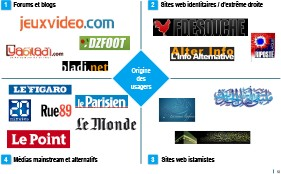
\includegraphics[width=3.88942in,height=2.3925in]{ImageIslamFrance/media/image10.jpeg}

L'islam sur YouTube


YouTube est un élément clé du débat avec énormément de contenu publié et
relayé en rapport avec l'islam. En particulier, des dizaines de chaînes
sont tenues par des imams francophones, atteignant des dizaines de
milliers d'abonnements.

À cela s'ajoute d'innombrables vidéos sensation -- caméras cachées,
séquence émotion à la Mecque, exorcismes, extraits de débats, images
choc -- ainsi que des vidéos de musique et de récitations du Coran ; ces
dernières sont les plus performantes en termes de nombre de vues,
puisqu'elles sont utilisées comme musique de fond et jouées à
répétition.

III. L'ISL AM « D'EN BAS »


L'offre idéologique islamique sur support vidéo Typologie et contenus


L'ensemble des discours auquel grand public a accès signale
l'\textbf{importance des}

\textbf{vidéos d'internet} dans la diffusion des idéologies islamistes.
Les vidéos les plus vues sur l'ensemble de la plateforme YouTube sont de
\textbf{cinq types} (par ordre décroissant en nombre de vues) :


\begin{itemize}
\item
  les r\textbf{écitations coraniques :} vidéos très longues (60 minutes
  ou plus), de loin les plus vues (16 000 000). Leur large consommation
  est certainement due à un visionnage en « bruit de fond » ;
\item
  les \textbf{« vidéo buzz »} : brèves, liées à des sujets d'actualité :

  \begin{itemize}
  \item
    \textbf{laïcité :} des jeunes musulmanes empêchées d'entrer dans
    leur lycée ou dans des magasins à cause leur habillement (voile,
    gants, robes longues, etc.),
  \item
    \textbf{« people » :} des interviews de personnalités (Karim Achoui,
    rappeurs, etc.),
  \end{itemize}
\item
  \textbf{questions identitaires :} échos du conflit israélo-palestinien
  (LICRA, LDJ), rejet institutionnel et des médias \emph{« mainstream
  »}, perçus comme racistes. Ces vidéos sont souvent les plus politiques
  ;
\item
  les \textbf{vidéos « émotionnelles »} : des vidéos très courtes, au
  contenu religieux presque accessoire ; spiritualités émotives et
  émerveillement sentimental plutôt que la doctrine ; abondance de
  scènes «miraculeuses» ou dramatiques (enfants émus par l'appel à la
  prière, pleurs, etc.) ;
\item
  les \textbf{animations « spirituelles »} : des animations ou des
  vidéos de paysages avec un narrateur parlant de sujets spirituels, le
  plus souvent eschatologiques (signes avant-coureurs de l'apocalypse,
  etc.), très longues (5 à 6 heures)128 ; \textbf{les prêches et les «
  conférences »} : faites par les « Imams YouTube » (15 min

  \begin{itemize}
  \item ~
    1 h)129. Ce sont les discours les plus consommés.
  \end{itemize}
\end{itemize}


Ces contenus diffusés sur YouTube n'offrent \textbf{pas une homogénéité
satisfaisante} pour les caractériser. Leurs points communs indiquent
cependant une \textbf{logique d'affirmation identitaire par le biais
d'islam(s)}. Cette construction identitaire est souvent explicitement
présentée comme étant en rupture avec certaines modernités qui
s'entremêlent :


\begin{itemize}
\item
  la consommation de masse ;
\end{itemize}


128 Exemple : \emph{L'au-delà !} (The Hereafter).

129 Exemples : Imam de Brest, Nader Abu Anas, Sheikh Al-Awadi (Kuweit).




\begin{itemize}
\item
  le rythme accéléré des communications qui détourne d'autrui et de ce
  qui est spirituel ;
\item
  un mode de vie jugé frivole, voire pécheur ;
\item
  des institutions perçues comme injustes ou hostiles.
\end{itemize}


L'immense majorité de ces productions proposent des contenus
difficilement compatibles avec les valeurs républicaines.


Des dynamiques de sens : construction d'un être au monde, d'interactions
du quotidien et du religieux


Les \textbf{vidéos de prêche} étonnent par la \textbf{trivialité de
leurs sujets.} Leur contenu n'est pas particulièrement heurtant pour le
grand public. Les questions traitées ont trait à des
\textbf{préoccupations courantes,} assez peu religieuses. Leur
\textbf{mise en scène} est très \textbf{simple}, parfois très
\textbf{théâtrale} (jeux de rôle caricaturaux), \textbf{emphatique}
(prêche depuis une tombe), et d'une \textbf{qualité technique très
limitée} (audio, vidéo et montage de faible qualité).

Les prêcheurs y répondent surtout à des questions au sujet de l'amour,
de conflits de couple, de \textbf{relations sexuelles,} de la
\textbf{réussite,} de l'\textbf{argent}, du rapport entre les
\textbf{parents et leurs fils,} de l'\textbf{amusement}. Les réponses
données sont assez semblables à celles que l'on attend de toute religion
sociale : les imams prônent la juste mesure, la bienveillance, la
générosité, la compréhension d'autrui, le dialogue, la tendresse, la
discipline.

Ce qui apparaît plus étonnant, c'est la \textbf{liturgie gestuelle et
verbale} orchestrant ces contenus triviaux. De l'ensemble des prêches
ressortent trois degrés de discours, accompagnés de dispositifs gestuels
:


\begin{itemize}
\item
  la plus grande partie de ces discours emprunte les \textbf{mots de la
  jeunesse} des banlieues. Très conscients du quotidien et des
  inquiétudes de leur auditoire, les orateurs veillent avec emphase à
  susciter l'adhésion à leur discours par des processus
  d'identification.
\item
  à ce discours du quotidien se mêle un \textbf{discours moral,
  théâtral, en français.}
\end{itemize}


Ce discours utilise un vocabulaire religieux, moral, au ton grave («
hélas »,

« miséricorde », « humilité ») ;


\begin{itemize}
\item
  le \textbf{troisième discours,} qui ponctue et \textbf{interrompt les
  deux précédents, est en arabe coranique.} Il s'agit de formules
  rituelles et de \textbf{récitations \emph{in extenso} de versets.}
\end{itemize}

\begin{enumerate}
\def\labelenumi{\Roman{enumi}.}
\setcounter{enumi}{2}
\item
  L'ISL AM « D'EN BAS »
\end{enumerate}


Ces trois discours s'entremêlent. Il en ressort un discours qui établit
le religieux comme quotidien, et le quotidien comme religieux :


\begin{itemize}
\item
  la parole coranique vient ponctuer le langage de tous les jours, le
  sacralisant ;
\item
  le langage quotidien se trouve empreint de religiosité dans ses
  signifiés les plus triviaux.
\end{itemize}


La grande force de ce discours découle de cette mise en scène du sens,
qui lui confère une autorité absolue. Tout est religieux, la religion
est partout.


Promesse véhiculée


Cette élaboration discursive explique l'attrait de cette sorte de prêche
salafiste. \textbf{La promesse} téléologique de ces discours
\textbf{n'est pas historiquement révolutionnaire.} Comme tous les
millénarismes, \textbf{elle affirme la prompte arrivée de la fin des
temps,} et la justice qui y sera rendue.

L'appel qui y est fait, est de mener une vie qui plaise à Allah, afin de
garantir son salut. Cette vie est présentée comme difficile en raison
\textbf{du déluge de péchés} modernes. L'enfer guette tant qu'y échapper
est déjà presque un paradis. \textbf{La promesse est celle d'une justice
implacable.}

Il convient pourtant de signaler que cette justice est double : elle
s'exerce dans l'au-delà, dans l'éventualité du jugement dernier, mais
aussi ici-bas.

De nombreuses histoires édifiantes promettent que le péché commis
entraînera un châtiment dès la vie terrestre du pécheur ; se mêlent
ainsi à nouveau le quotidien et le transcendant, dans un être au monde
construit sur cette idée : \textbf{le trivial compte autant que le
religieux, le religieux est trivial, gestuel.} Le salut de l'âme se joue
chaque jour, chaque jour peut le mettre en péril.

En ce sens, la vie proposée est presque sans promesse : elle se promet
elle- même. Vivre comme le prophète et les \emph{salaf as-salih} est
déjà le paradis.

La réalité de l'islam français, avant d'être institutionnelle, est
d'abord locale et quotidienne. C'est un islam parcellaire, fragmenté et
éclaté, mais en voie d'intégration et de structuration au niveau local
qui se dessine. L'arrivée du



salafisme et sa visibilité attestent, paradoxalement, de la relative
bonne intégration de l'islam dans le paysage national. Parce qu'il se
fond dans le quotidien, l'islam des collectivités est difficile à
appréhender : il offre peu de de traits saillants à analyser et s'avère
être, par conséquent, un objet peu étudié ; seuls les mouvements
radicaux et minoritaires sont visibles. L'émergence rapide du salafisme
montre également, ainsi que le notait déjà en 2005 Samir Amghar, que
\emph{« la France est devenue un maillon de la globalisation du
religieux musulman, et constitue une plaque tournante pour de nombreux
flux transnationaux islamiques. Dans un tel contexte, comment concevoir
le contrôle de l'État, qu'il soit français ou qu'il s'agisse de l'État
d'origine ? La transnationalisation provoque une transformation des
relations entre l'islam et l'État, en de nouvelles formes d'autonomie et
de concurrence. La transnationalisation et la déterritorialisation des
mouvements islamiques donnent le primat aux leaders religieux et aux
chefs charismatiques, comme nous l'avons vu avec les théologiens
salafistes}130\emph{. »}

Ce mouvement de transnationalisation et de déterritorialisation s'est
considérablement renforcé avec la démocratisation de l'accès à internet
et l'apparition des réseaux sociaux. Cette évolution de l'islam français
rend ainsi d'autant plus difficile, et d'autant plus urgent, le travail
de structuration de l'islam en France à la fois par les musulmans de
France et par la puissance publique.

130 Samir Amghar, Acteurs internationaux.


\hypertarget{iv}{%
\subsection{IV}\label{iv}}

\hypertarget{pistes-de-recommandations}{%
\subsubsection{PISTES DE
RECOMMANDATIONS}\label{pistes-de-recommandations}}


L'analyse du paysage de l'islam français permet d'éclairer la faiblesse
organisationnelle de l'islam en France. En partie soumis aux influences
étrangères, il peine à se structurer et à s'organiser. Les musulmans de
France, parce qu'ils forment une

« communauté introuvable », parce qu'ils présentent une grande diversité
à la fois ethnique et sociodémographique, ne parviennent pas à se doter
des structures nécessaires pour une gestion à la fois transparente,
structurée et régulée de l'islam français.

Les fondamentalistes ont pris une avance considérable dans plusieurs
domaines, mais, d'abord et avant tout, dans la diffusion de leur
idéologie. Dès lors, le combat doit être idéologique et culturel. Il
faut utiliser tous les moyens en notre possession pour soutenir les
musulmans dans le travail nécessaire qu'ils doivent mener
d'interprétation des textes et de diffusion des connaissances.
\textbf{La connaissance et la culture sont les enjeux premiers.}

\textbf{Le deuxième enjeu est le financement et l'organisation.} L'islam
de France est sous-financé, mal organisé et laisse place à des
offensives de groupes militants qui n'ont pas besoin de beaucoup de
moyens pour s'imposer, dans les mosquées et sur internet. Il faut donc
financer et organiser de façon transparente l'islam de France en
inventant, enfin, les moyens de s'affranchir des tutelles étrangères

Enfin, l'État doit comprendre que les mieux à même de gérer l'islam en
France, ce sont les Français, et non les États d'origine ni un CFCM dans
lequel les musulmans ne se reconnaissent pas. Il faut donc leur
permettre d'engager ces changements.




\hypertarget{propositions}{%
\paragraph{4.1. PROPOSITIONS}\label{propositions}}

\hypertarget{ruxe9ussir-la-cruxe9ation-de-la-fondation-pour-lislam-de-france-lassociation-musulmane-pour-un-islam-de-france-deux-institutions-majeures}{%
\subparagraph{Réussir la création de la Fondation pour l'islam de
France, l'association musulmane pour un islam de France : deux
institutions
majeures}\label{ruxe9ussir-la-cruxe9ation-de-la-fondation-pour-lislam-de-france-lassociation-musulmane-pour-un-islam-de-france-deux-institutions-majeures}}


L'islam en France est confronté à un double défi : sortir enfin de la
tutelle des États étrangers et centraliser son organisation, avec
l'intérêt général des Français de confession musulmane comme principe
directeur.

L'islam de France doit devenir français. Il ne l'est pas aujourd'hui.
Les personnes qui le gèrent et celles qui représentent les musulmans
français sont encore étroitement liées aux États d'origine. Elles ont
importé les tensions qui existent entre certains États du Maghreb, ne
connaissent pas bien les jeunes Français avec qui elles sont pourtant
censées travailler et ne maîtrisent pas les outils de communication de
la jeunesse française.

Pourtant, trois musulmans sur quatre sont désormais des Français (dont
50 \% de naissance). Une nouvelle génération de musulmans français a
grandi en France et dispose d'un haut niveau de formation. Pour que
l'islam français puisse se doter d'une ligne théologique compatible avec
la société française et afin qu'il puisse rompre avec les discours
diffusés par les États émetteurs d'idéologies rigoristes, il faut créer
des instances capables de produire et de diffuser des idées et des
valeurs françaises.

Extrêmement fragmenté et divisé entre les États d'origines, les
mouvements transnationaux et les acteurs locaux, l'islam français doit
faire sa mue : il faut


\begin{enumerate}
\def\labelenumi{\Roman{enumi}.}
\setcounter{enumi}{3}
\item
  
  PISTES DE RECOMMAND ATIONS
  
\end{enumerate}


centraliser sa gestion afin de la rendre plus lisible et plus
efficiente. Cette maturation de l'islam français requiert aussi une
centralisation des moyens, un accroissement des capacités financières,
un effort de transparence et un contrôle accru avec un seul objectif :
l'intérêt général des musulmans de France et leur adhésion au pacte
républicain.

En août 2016, le ministre de l'Intérieur a annoncé la création d'une
Fondation pour l'Islam de France, dont Jean-Pierre Chevènement,
présidera le volet culturel131. Ses principales missions seront la
formation des imams et la production de connaissances sur l'islam.

Il faudra lui accoler une association cultuelle régie par la loi de 1905
pour pouvoir financer ce qui est du strict ressort cultuel (construction
des lieux de culte, salariat des imams, formation théologique). Le
Conseil d'État a contesté le fait qu'une fondation d'utilité publique
puisse contribuer au financement du culte On pourrait appeler cette
association « l'association musulmane pour un islam de France (AMIF) ».
Pour y parvenir, il faut proposer une nouvelle gouvernance et une
nouvelle génération pour les deux organisations.

\textbf{Trois propositions pour la gouvernance et l'organisation de ces
deux institutions.}


Gouvernance proposée pour ces deux institutions


Ainsi, pour leur premier mandat, au conseil d'administration de ces
organisations, une majorité de ces Français de confession musulmane
devront être cooptés par l'État. Pourquoi par l'État ? Parce qu'il
s'agit d'une fondation reconnue d'utilité publique, et parce que l'État
aura conféré à l'association le monopole de la délivrance de carte de
certification, permettant ainsi le monopole religieux. Mais aussi parce
que l'État devra assumer la nécessité de renouveler à la fois les
générations et l'organisation. Cette nouvelle génération siègera avec, à
ses côtés, des représentants du CFCM qui devront être
\textbf{minoritaires} dans l'organisation.

Ces nouveaux membres, capables de fédérer la communauté musulmane et de
lever des fonds pour le financement du culte musulman, auront une double
mission : centraliser les flux financiers liés à l'exercice de la
religion et organiser

131 On ne peut que s'étonner qu'une personnalité non musulmane préside
la Fondation de l'islam de France. Cependant, Jean-Pierre Chevènement
pourra être le préfigurateur de la Fondation, en lien avec le futur
président de l'association cultuelle, avant de passer la main dans un
délai aussi bref que possible à une personnalité musulmane.



l'emploi efficace et transparent de ces ressources. Le Conseil
d'administration des deux organisations ainsi nommé aura également pour
mission de mettre au point le dispositif qui permettra de renouveler sa
composition au terme de ce premier mandat, \emph{via} un système
représentatif


Une nouvelle équipe


La réactivation de la FIF et la création de l'AMIF devront s'accompagner
d'un profond renouvellement des représentants et des acteurs de l'islam
français. Il est temps de faire émerger \textbf{une nouvelle génération
de musulmans, qui ont grandi et ont été socialisés en France et de
profiter de la volonté qu'ils ont manifestée.} Il revient à la puissance
publique d'accompagner l'émergence de cette nouvelle génération de
musulmans français, en la nommant au conseil d'administration et à la
direction générale de la Fondation ; aux côtés de membres du CFCM, qui
ne devront composer que moins de la moitié du Conseil d'administration
de la FIF et de l'AMIF. Cette nouvelle génération devra également
investir les conseils régionaux de la Fondation, qui seront composés de
personnalités désignées, pour ce premier mandat, par les autorités
publiques et des membres du CFCM.


Une mission principale : centraliser les flux financiers


\textbf{La Fondation pour l'islam de France (FIF) et l'AMIF,} doivent
devenir la clef de voûte de la nouvelle gestion de l'islam français.
Forte de l'ensemble des financements liés à l'exercice religieux, l'AMIF
financera les lieux de culte, formera et salariera les imams et
financera le travail théologique. La Fondation limitera le champ de son
action au domaine culturel. Ces revenus financiers procèderaient de
quatre sources différentes :


\begin{itemize}
\item
  \textbf{le monopole des cartes de sacrificateurs musulmans.}
  Actuellement, trois mosquées (liées pour deux d'entre elles
  explicitement à des pays étrangers, l'Algérie pour la mosquée de Paris
  et le Maroc pour la mosquée d'Évry) bénéficient d'un agrément donné
  par le ministère de l'Agriculture sur proposition du ministère de
  l'Intérieur pour délivrer des cartes de sacrificateurs religieux. Ces
  sacrificateurs rendent un service qui est rémunéré par les abattoirs
  dont le produit sert au financement des mosquées qui en bénéficient et
  des associations qui leur sont proches.
\end{itemize}


L'AMIF (l'association cultuelle) devra être demain la seule titulaire de
l'agrément afin de pouvoir centraliser les flux financiers liés à
l'abattage \emph{halal} (quitte à passer par une structure juridique
\emph{ad hoc} si besoin est). L'AMIF s'engagera à reprendre les

IV. PISTES DE RECOMMAND ATIONS

sacrificateurs qui travaillent actuellement pour les mosquées agréées et
proposera aux mosquées une compensation sur une base transparente, pour
autant que le produit actuel du service des sacrificateurs serve la
communauté musulmane.

L'AMIF (association loi de 1905), seule titulaire de l'agrément, pourra
ensuite faire évoluer les tarifs des sacrificateurs, dans l'intérêt des
fidèles, après avoir évalué les besoins de financement du culte musulman
en France et les différentes sources de recettes.

Il y aura bien sûr des difficultés (pourquoi augmenter le prix des
services ? pourquoi retirer l'agrément à des mosquées qui n'ont pas
démérité ? pourquoi prélever plus d'argent sur des gens disposant
souvent de peu de ressources ?) mais, avec le service de certification,
la redevance pour l'abattage \emph{halal} est une source majeure de
financement qu'il faut utiliser jusqu'au bout ;


\begin{itemize}
\item
  \textbf{une offre de certification \emph{halal} sur toute la chaine de
  valeurs.} Il est impossible de créer une taxe halal, compte tenu du
  périmètre fluctuant de la définition du halal, du respect nécessaire
  de la liberté de commerce et de la concurrence, et du principe
  constitutionnel d'égalité des citoyens devant l'impôt. Il est
  toutefois possible de doter l'AMIF d'une mission de certification du
  \emph{halal} sur l'ensemble de la chaîne de valeur, qui viendrait
  concurrencer les acteurs déjà présents sur ce marché. Conformément au
  droit de la concurrence et au respect de la liberté d'entreprendre,
  l'AMIF n'aurait pas le monopole de la certification du \emph{halal},
  mais aurait à charge de savoir déployer un vrai service de
  certification en se fondant sur sa légitimité nationale, sur la
  transparence de ses coûts et surtout sur l'utilisation de ses
  bénéfices au service de la collectivité ;
\item
  l\textbf{e recueil des dons versés par des pays ou des personnalités
  étrangères.} Il règne actuellement une véritable opacité autour des
  dons versés par les pays et les personnalités étrangères aux
  associations musulmanes. Il est nécessaire d'introduire de la
  transparence, et surtout de rompre l'affiliation de certaines
  associations avec les pays d'origine. C'est pourquoi ces flux
  financiers devront être progressivement réorientés et transiter
  obligatoirement par la FIF, afin de permettre une centralisation -- en
  toute transparence -- du financement étranger de l'islam français ;
\item
  \textbf{le recueil d'une redevance sur le pèlerinage,} en lien avec
  les agences de voyage qui l'organisent ;
\end{itemize}





\begin{itemize}
\item
  \textbf{le recueil de dons (zakat) venus des fidèles français.} La
  zakat représente, tout comme les financements étrangers, une
  importante source de financement de l'islam français. Or, ce mode de
  financement est totalement opaque, fragmenté et parcellaire. Il est
  nécessaire d'y introduire de la transparence, et surtout de mutualiser
  au sein de la Fondation les ressources provenant des fidèles : cette
  centralisation du financement des fidèles permettra à l'islam français
  de se structurer et de se professionnaliser ; et par là même de mieux
  s'intégrer dans la République. On pourra imaginer d'utiliser des
  moyens modernes de dons, comme par exemple des applications sur
  smartphones.
\end{itemize}


L'AMIF sera des deux organisations celle qui aura vocation à recueillir
le plus d'argent, les besoins de financement étant essentiellement liés
à l'exercice du culte. La Fondation pourra recevoir des dons de
personnes physiques, sachant que son action sera strictement limitée au
domaine culturel, conformément à la loi de 1905 et à la séparation de
l'Église et de l'État.


L'usage des fonds


Les fonds recueillis et centralisés par la FIF auront plusieurs emplois
:


\begin{itemize}
\item
  \textbf{financer la construction de lieux de culte :} toute
  construction de mosquée devra être préalablement visée par la FIF et
  son plan de financement certifié par son équipe dirigeante ;
\item
  \textbf{salarier les imams :} tout imam ayant passé avec succès le «
  Test de l'islam français » (détail ci-après) administré par l'AMIF
  pourra être salarié par cette association. La centralisation des
  ressources et la garantie d'un discours théologique compatible avec
  les valeurs et les principes de la République permettront l'émergence
  d'un islam français ;
\item
  \textbf{former les imams :} en plus de la reconnaissance -- ou non --
  des imams déjà en fonction, la Fondation aura pour mission de former
  une nouvelle génération d'imams. La centralité de l'AMIF, clef de
  voûte de l'islam français, permettra ainsi de mettre fin à la
  délégation de la formation des imams à des pays étrangers ou à des
  instituts privés. L'objectif est de garantir que les tous les imams en
  France soient français -- ou maîtrisent le français -- et aient suivi
  la formation d'une institution reconnue par la République et
  compatible avec ses idéaux ;
\end{itemize}


IV. PISTES DE RECOMMAND ATIONS


\begin{itemize}
\item
  \textbf{rémunérer l'équipe de l'AMIF, de la Fondation et des
  sacrificateurs :} la FIF, en plus de la rémunération des personnes
  chargées du fonctionnement administratif de l'islam français, devra
  salarier les sacrificateurs \emph{halal} auxquels elle aura délivré
  des accréditations ;
\item
  \textbf{engager un travail idéologique :} à terme, une fois la
  centralisation des flux financiers durablement assurée et les
  institutions nécessaires à l'émergence d'un islam français solidement
  implantées, la FIF aura pour mission d'engager une véritable bataille
  culturelle, sur le web et sur le terrain, afin de réduire l'emprise
  des discours islamistes, salafistes et djihadistes sur les musulmans
  de France.
\end{itemize}


La réactivation de la FIF, la création de l'AMIF, la centralisation des
flux financiers, un usage responsable des fonds et l'arrivée d'une
nouvelle génération de musulmans français doivent permettre l'émergence
d'un islam français, mais aussi de mettre un terme à sa fragmentation et
à sa gestion externalisée, afin d'être en mesure de répondre aux défis
auxquels il fait face aujourd'hui.


\hypertarget{un-grand-imam-de-france-pour-exprimer-une-doctrine-musulmane-compatible-avec-les-valeurs-ruxe9publicaines}{%
\subparagraph{Un grand imam de France pour exprimer une doctrine
musulmane compatible avec les valeurs
républicaines}\label{un-grand-imam-de-france-pour-exprimer-une-doctrine-musulmane-compatible-avec-les-valeurs-ruxe9publicaines}}


Afin de désigner un interlocuteur musulman légitime et représentatif aux
pouvoirs publics, nous recommandons l'élection d'un Grand Imam de
France. Celui-ci devra être de nationalité française, diplômé de
théologie, imam d'une mosquée et avoir recueilli le parrainage de
présidents d'associations cultuelles. Il sera élu par le Conseil
d'administration de l'AMIF et, éventuellement, un collège élargi avec
des personnalités qualifiées. Il portera un discours et une ligne
idéologique qui puisera au plus profond des valeurs spirituelles de
l'islam tout en étant en adéquation avec la société française du XXIe
siècle. Il sera le représentant spirituel de l'islam français

-- aux côtés des présidents du CFCM et de l'AMIF --et aura pour mission
d'intervenir, à l'instar du Grand Rabbin de France, dans les médias --
ou auprès d'institutions désireuses de recueillir un éclairage
théologique sur certaines questions -- afin de mieux faire connaître
l'islam. Il devra également conduire le travail intellectuel et
théologique destiné à poser les jalons d'un islam français. Pour cela,
il devra interagir avec tous les imams de France. Il pourra, en accord
avec l'AMIF, les révoquer en



cas de discours déviant ou de prises de positions contraires au
vivre-ensemble. Il s'appuiera pour cela sur des représentants religieux
régionaux.

Si le Grand Imam de France sera chargé de représenter les ministres du
culte musulman, les responsables de l'AMIF auront également pour mission
d'être le visage des musulmans français et de parler au nom de cette
majorité silencieuse, bien intégrée dans la République française et
première victime de l'islamisme et du radicalisme religieux.


\hypertarget{uxe9largissement-du-concordat-alsaco-mosellan-uxe0-lislam}{%
\subparagraph{Élargissement du concordat alsaco-mosellan à
l'islam}\label{uxe9largissement-du-concordat-alsaco-mosellan-uxe0-lislam}}


\textbf{Un régime particulier conforté par le législateur, le Conseil
d'État et le Conseil constitutionnel}

L'Alsace-Moselle jouit d'un régime cultuel différent de celui du reste
de la métropole : la loi de 1905 ne s'y applique pas. Cette
particularité s'explique par la situation de ces départements qui
étaient sous occupation allemande en 1905. Conformément aux dispositions
qui courraient avant l'application de la loi de 1905, les quatre cultes
« reconnus » (le culte catholique, les cultes protestants luthérien et
réformé et le culte judaïque) sont pris en charge par la puissance
publique, qui finance l'intégralité du culte, nomme et révoque les
ministres du culte, et assure pour chacun de ces cultes un enseignement
religieux (facultatif aujourd'hui) à l'école publique.

\textbf{Cette disposition dérogatoire au droit commun n'a pas été remise
en cause} et a été entérinée par la loi du 1er juin 1924132 et par un
avis du Conseil d'État en 1925133. Ce régime juridique applicable aux
cultes en Alsace-Moselle a été réaffirmé à plusieurs reprises depuis.
L'ordonnance du 15 septembre 1945, en maintenant en vigueur le droit
applicable le 16 juin 1940, confirme l'application du régime
concordataire en Alsace-Moselle. En 2001, dans sa décision
\emph{Syndicat national des enseignements du second degré,} le Conseil
d'État a également rappelé que \underline{les principes fondamentaux
reconnus par les lois de la République, au nombre}

132 Loi du 1er juin 1924 mettant en vigueur la législation civile
française dans les départements du Bas-Rhin, du Haut- Rhin et de la
Moselle, art. 7.

133 CE, sections réunies de la Législation, de la Justice et des
Affaires étrangères et de l'Intérieur, de l'Instruction publique et des
Beaux-arts, avis n°188.150 du 24 janvier 1925

IV. PISTES DE RECOMMAND ATIONS

desquels figure le principe de laïcité dans les préambules des
constitutions des 27 octobre 1946 et 4 octobre 1958 \emph{« n'a pas eu
pour effet d'abroger implicitement les dispositions de ladite loi ».}

Dernièrement, en 2013, c'est le Conseil constitutionnel qui a confirmé
la constitutionnalité de cette disposition particulière. Ainsi, à
l'occasion de la question prioritaire de constitutionnalité (QPC)
\emph{Association pour la promotion et l'expansion de la laïcité,}
\textbf{le juge constitutionnel a affirmé à son tour que le régime
concordataire qui prévaut encore en Alsace-Moselle n'est pas entaché
d'inconstitutionnalité}134\textbf{.}


La situation de l'islam dans le régime concordataire


Aujourd'hui, \textbf{l'islam n'est pas intégré au régime concordataire}
alsacien et mosellan. C'est \textbf{un culte « non-reconnu ».} Par
conséquent, le financement du culte musulman -- et plus largement celui
des nouveaux cultes -- n'est pas aligné sur le régime dont bénéficient
les quatre cultes reconnus. En revanche, \textbf{les associations -- en
vertu du droit local -- peuvent recevoir des soutiens financiers publics
et les collectivités peuvent participer au financement d'une partie des
cultes non-reconnus} (en respectant cependant un certain nombre de
règles). C'est ainsi que la mairie de Strasbourg, le département du
Bas-Rhin et la région Alsace ont participé au financement de la
construction de la Grande Mosquée de Strasbourg à hauteur de 1,6 million
d'euros, soit un quart du coût total de l'édifice. Toutefois, le régime
concordataire empêche les pouvoirs publics de prendre en charge la
totalité du culte et de pouvoir nommer et salarier des imams. Pour ainsi
dire, \textbf{si la puissance publique peut en partie financer le culte
musulman en Alsace-Moselle, elle ne peut en revanche pas en réguler le
fonctionnement.}

\textbf{Parce que le régime concordataire est protégé aussi bien par le
législateur que par le Conseil d'État ou le Conseil Constitutionnel,
certains ont envisagé d'y intégrer l'islam, afin de permettre aux
pouvoirs publics de participer plus avant au fonctionnement de ce
culte.} Cette idée n'est pas nouvelle. Déjà, en 1997, alors qu'il était
au ministère de l'Intérieur, Jean-Pierre Chevènement songeait à utiliser
ce régime dérogatoire pour en faire un laboratoire de l'islam français
et créer une université de théologie islamique à Strasbourg.

134 CC, Décision n'° 2012-297 QPC du 21 février 2013. Voir notamment le
sixième considérant : « \emph{Considérant, toutefois, qu'il ressort tant
des travaux préparatoires du projet de la Constitution du 27 octobre
1946 relatifs à son article 1er que de ceux du projet de la Constitution
du 4 octobre 1958 qui a repris la même disposition, qu'en proclamant que
la France est une ``République. . . laïque'', la Constitution n'a pas
pour autant entendu remettre en cause les dispositions législatives ou
règlementaires particulières applicables dans plusieurs parties du
territoire de la République lors de l'entrée en vigueur de la
Constitution et relatives à l'organisation de certains cultes et,
notamment, à la rémunération de ministres du culte ; »} (nous
soulignons).



C'est également l'idée du député François Grosdidier lorsqu'il dépose,
en 2006, une proposition de loi visant à intégrer le culte musulman dans
le régime concordataire d'Alsace et de Moselle afin de mettre fin à une
situation inégalitaire. Selon lui, étant donné \textbf{que les nouveaux
cultes, au premier rang desquels l'islam, se trouvent dans une situation
défavorable au regard de celle des cultes reconnus dans les trois
départements de l'Est,} il se prononçait en faveur \emph{\textbf{« d'une
actualisation de la loi concordataire »}} en direction de l'islam.
Reprenant l'idée développée par Jean- Pierre Chevènement, il se
prononçait également en faveur de la création d'une chaire de théologie
islamique à l'université de Strasbourg, dont les travaux pourraient
contribuer à l'émergence d'un islam français.

Au-delà des raisons politiques qui ont conduit au non-examen de ce texte
et des raisons juridiques -- du risque d'inconstitutionnalité de cette
proposition de loi --, \textbf{le Conseil Constitutionnel a clos jusqu'à
nouvel ordre le débat public autour de cette question en 2011.} En
effet, dans sa décision \emph{Société SOMODIA,} relative à
l'actualisation du régime concordataire en Alsace et Moselle, il a
rappelé que si le législateur ou le pouvoir réglementaire pouvaient
maintenir, atténuer ou même supprimer les dispositions du droit local,
\textbf{ils ne pouvaient pas en revanche, en élargir le champ
d'application.} Si la dérogation au droit commun demeure l'exception,
son approfondissement n'est pas souhaitable, car il risquerait
d'accroître l'inégalité des citoyens devant la loi. \textbf{Le juge
constitutionnel a signifié ainsi que les cultes nouvellement installés
sur le territoire français ne peuvent, en Alsace- Moselle, bénéficier du
même régime juridique que les cultes reconnus}135\textbf{.} Ainsi, en
2011, le Conseil Constitutionnel a fermé la voie à toute tentative de
faire de l'Alsace-Moselle un théâtre d'expérimentation et le lieu
d'émergence d'un islam

\emph{« made in France ».}

135 Décision n°2011-157 QPC du 5 août 2011. Voir notamment le quatrième
considérant : Considérant qu'ainsi, la législation républicaine
antérieure à l'entrée en vigueur de la Constitution de 1946 a consacré
le principe selon lequel, tant qu'elles n'ont pas été remplacées par les
dispositions de droit commun ou harmonisées avec elles, des dispositions
législatives et réglementaires particulières aux départements du
Bas-Rhin, du Haut-Rhin et de la Moselle peuvent demeurer en vigueur ;
qu'à défaut de leur abrogation ou de leur harmonisation avec le droit
commun, ces dispositions particulières ne peuvent être aménagées que
dans la mesure où les différences de traitement qui en résultent ne sont
pas accrues et que leur champ d'application n'est pas élargi ; que telle
est la portée du principe fondamental reconnu par les lois de la
République en matière de dispositions particulières applicables dans les
trois départements dont il s'agit ; que ce principe doit aussi être
concilié avec les autres exigences constitutionnelles » (nous
soulignons)

IV. PISTES DE RECOMMAND ATIONS


Nécessité et modalités d'intégration de l'islam au régime concordataire

Nécessité


Il est, aujourd'hui plus que jamais, nécessaire \textbf{d'intégrer
l'islam au régime concordataire.} Il ne s'agit pas de faciliter le
financement du culte musulman, mais de créer un écosystème politique et
juridique qui permette aux instances représentatives des musulmans de
France et à la puissance publique de \textbf{faire émerger un islam
français,} dont les discours et la pratique soient en adéquation avec
les évolutions de notre société.

L'actualisation du régime concordataire doit offrir la possibilité de
\textbf{créer une chaire de théologie musulmane} à l'Université de
Strasbourg, dont la mission consisterait à produire de la connaissance
sur l'islam à destination des Français, ainsi qu'à élaborer un discours
théologique compatible avec les attentes de la société et les exigences
de la République.

L'Alsace-Moselle pourrait également accueillir \textbf{une école de
formation des imams.} En créant un diplôme français de théologie
islamique, l'État répondrait à une forte attente des musulmans de
France. Surtout il se donnerait les moyens, sur le temps long, de
diffuser auprès des fidèles musulmans un discours adapté aux valeurs de
notre société.


Modalités


\emph{Revenir sur la jurisprudence Société Somodia}

L'intégration de l'islam au régime concordataire implique, tout d'abord,
de \textbf{revenir sur la jurisprudence du Conseil constitutionnel.} En
effet, si en 2011 le juge constitutionnel avec la décision sur le QPC
\emph{Société Somodia} a sécurisé le droit local des cultes
(sécurisation qui sera confirmée en 2013 avec la QPC \emph{Association
pour la promotion et l'expansion de la laïcité}), il a en revanche
\textbf{verrouillé toute possibilité d'actualisation du droit
concordataire :} l'intégration de nouveaux cultes dans le régime
concordataire constituerait un approfondissement et un élargissement
trop important d'un droit local par nature dérogatoire.

Cette actualisation du régime concordataire implique donc de recourir à
une loi, \textbf{afin que celle-ci soit déférée devant le Conseil
constitutionnel,} et non d'emprunter la voie réglementaire au risque de
voir le Conseil d'État censurer le texte en raison de



son inconstitutionnalité manifeste. Il faut ensuite que \textbf{les
juges constitutionnels}

-- au regard des circonstances présentes et des dispositions du projet
de loi -- \textbf{procèdent à un revirement de jurisprudence.} Cette
évolution jurisprudentielle pourrait s'opérer autour de la nécessité de
réduire l'inégalité de situation à laquelle sont confrontés les fidèles
des cultes reconnus et ceux des cultes non-reconnus et qui porte
potentiellement atteinte à la liberté de culte -- et non autour de
l'application uniforme du droit sur l'ensemble du territoire ou de
l'objectif de réduction des dispositions particulières dérogatoire au
droit commun, qui structurent la décision \emph{Société Somodia}. Le
nouveau contexte politique et social, né des attentats de 2015 et de
2016, pourrait justifier cette évolution.

\textbf{Cette évolution jurisprudentielle serait loin d'être anodine,
car le Conseil constitutionnel n'est jamais revenu sur une décision
prise dans le cadre d'une QPC.} Assurément, ce revirement ferait
jurisprudence et risquerait fort d'agiter la doctrine juridique. Aussi,
au-delà des considérations politiques que soulève l'intégration de
l'islam au régime concordataire, il convient de \textbf{prendre en
compte l'ensemble des obstacles juridiques que rencontrera cette
proposition.}

\textbf{Comment « reconnaître » le culte musulman ?}

\textbf{Le terme de « reconnaissance » est impropre,} ainsi que le
rappelle fort à propos le rapport rédigé par Jean-Pierre Machelonde 2006
: \emph{« aucune loi n'a jamais reconnu explicitement les cultes
catholique, protestant et israélite. En revanche, ceux-ci ont engagé au
cours du XIXe siècle des négociations avec l'État débouchant, après une
période plus ou moins longue (50 ans pour le culte israélite) sur ce qui
peut être qualifié « d'arrangements statutaires ». Ces statuts
particuliers sont donc propres à chaque culte. {[}\ldots{]} Les cultes
statutaires ne constituent donc pas un ensemble homogène, et l'islam,
avec ses caractéristiques particulières, peut sans nul doute y trouver
sa place}136\emph{. »}

\textbf{Ce rapport publié en 2006, soit avant la QPC \emph{Société
Somodia,} propose de procéder à la « reconnaissance » du culte musulman}
en recourant à des dispositions règlementaires (recrutement des
ministres du culte musulman, création d'établissements du culte
musulman, etc.) afin d'amorcer un effet « cliquet » et de faciliter
l'introduction d'autres dispositions, qui relèvent de matières
législatives. Compte tenu de l'état actuel du droit et de la situation
jurisprudentielle, l'introduction

136 Rapport Machelon, p. 70 et 71.

IV. PISTES DE RECOMMAND ATIONS

du culte musulman dans le régime concordataire ne saurait s'effectuer de
manière

\emph{« pragmatique et progressive ».} Il faut d'emblée se situer au
niveau législatif afin que le texte soit visé par le Conseil
constitutionnel.

Par ailleurs, au regard de l'exigence de neutralité de l'État à l'égard
des cultes et de son corollaire -- l'égalité de traitement des
différents cultes qui prévalent dans les régimes juridiques dérogatoires
au droit commun des cultes137 --, \textbf{il importe de veiller à ce que
le texte législatif visant à élargir à l'islam le régime concordataire
ne soit pas exclusif au seul culte musulman.} Par conséquent, s'il faut
procéder à l'actualisation du concordat alsacien-mosellan, il convient
de \textbf{l'ouvrir à l'ensemble des nouveaux cultes qui le
souhaiteraient} -- soit, compte tenu des pratiques cultuelles locales,
le culte orthodoxe, le culte protestant évangéliste et le culte
musulman, principalement.

C'est pourquoi, conformément à l'article 34 de la Constitution, deux
pistes non exclusives paraissent envisageables :


\begin{enumerate}
\def\labelenumi{\alph{enumi}.}
\item
  compte tenu du fait que les textes relatifs au droit local
  d'enseignement religieux ne se réfèrent pas à la notion de « cultes
  reconnus », \textbf{un projet ou une proposition de loi relatifs à la
  création de postes de professeurs non contractuels d'enseignement des
  religions musulmane,} orthodoxe et évangéliste permettraient au
  Conseil constitutionnel d'examiner le texte et de se prononcer en
  faveur d'un éventuel revirement de jurisprudence ;
\item
  
  en collaboration avec le CRCM, qui constitue l'instance représentative
  locale des musulmans, et \textbf{dans le cadre d'une loi de finance,
  un amendement relatif à la rémunération des ministres des cultes
  musulman,} orthodoxe et évangéliste, doit offrir la possibilité au
  Conseil constitutionnel -- dans le cadre de l'examen de
  constitutionnalité du PLF -- d'effectuer un revirement de
  jurisprudence sur le régime applicable au culte en Alsace-Moselle.
  
\end{enumerate}


Il est évident que ces deux voies ne constituent qu'\textbf{une première
étape dans la création d'un statut du culte musulman} et que leur
ambition est plus large que la structuration du seul culte musulman. Il
s'agit toutefois d'un passage obligé avant la création d'un véritable
écosystème politique, juridique et intellectuel propice à l'émergence
d'un islam français. Sans cette étape législative déterminante, il sera
\underline{impossible de mettre en place ultérieurement une formation
diplômante en théologie}

137 CE, 16 mars 2005, n° 265560, ministre de l'Outre-Mer c/ président de
la Polynésie française.



desdits professeurs non contractuels, ni de créer une chaire de
théologie islamique au sein de l'Université de Strasbourg.


Risques


Quels sont les risques que présente l'élargissement du régime
concordataire à de nouveaux cultes ? Si \emph{a priori} une telle mesure
ne soulève pas de véritable risque financier (voir après) et si le
risque juridique d'inconstitutionnalité est levé, les principaux risques
qui pèsent sur cette mesure sont politiques.


\begin{enumerate}
\def\labelenumi{\alph{enumi}.}
\item
  Cette mesure suscitera sans aucun doute \textbf{l'opposition des
  partisans de l'abolition du régime concordataire, qui ne sont pas
  favorables à une prise en charge des cultes par la puissance
  publique.} Il est indéniable que c'est une opposition à prendre en
  compte, et qui sera particulièrement virulente à l'occasion de
  l'examen des textes de lois.
\item
  
  \textbf{L'opposition des cultes « reconnus » dans le cadre du régime
  concordataire doit également être intégrée.} Ils exprimeront une
  double crainte. Ils risquent de voir dans cette mesure un risque de
  péréquation budgétaire défavorable à leur égard, d'une part ; ils ne
  manqueront pas d'agiter la menace d'un risque de rupture du régime
  concordataire, d'autre part. Son extension signifierait alors son
  abrogation. Toutefois, la décision de 2013 du Conseil Constitutionnel
  constitue une véritable sécurisation, au plus haut niveau
  juridictionnel, de ce dispositif politique et juridique.
  
\item
  
  Enfin, il est très probable qu'\textbf{une partie des musulmans sera
  opposée à la gestion du culte par la puissance publique.} L'offre
  consulaire est relativement importante en Alsace-Moselle, où les
  musulmans sont principalement d'origines marocaine et turque : la
  création d'un corps de fonctionnaires français en charge du culte
  musulman et l'émergence consécutive d'une offre d'islam français
  entraîneront des perturbations locales et diplomatiques qu'il convient
  d'anticiper afin de les atténuer. En outre, certains responsables
  d'associations cultuelles locales seront réticents face à une telle
  implication de l'État dans les affaires cultuelles, \textbf{car la
  prise en charge publique des cultes implique en contrepartie un
  important droit de regard et de contrôle de leur fonctionnement.}
  
\end{enumerate}


IV. PISTES DE RECOMMAND ATIONS


Coût de l'élargissement du régime concordataire à l'islam


\textbf{Le coût d'une telle mesure s'établirait entre 5,5 et 6 millions
d'euros,} et se répartirait comme suit :


\begin{itemize}
\item
  au regard de la population musulmane et du nombre de mosquées en
  Alsace- Moselle, il faudrait procéder à la rémunération d'\textbf{une
  soixantaine de fonctionnaires du culte,} qui pourront assurer aussi
  bien la formation religieuse scolaire que le ministère du culte. Avec
  un salaire mensuel compris entre 1 800 et 2 000 e, \textbf{nous
  estimons que la création d'un corps de fonctionnaires du culte
  musulman s'élèverait à 2,5 millions d'euros par an environ ;}
\item
  la \textbf{création d'une chaire de théologie islamique au sein de
  l'Université de Strasbourg,} qui compterait dans un premier temps une
  petite dizaine de professeurs, est estimée \textbf{entre 1 million et
  1,5 million d'euros par an ;}
\item
  enfin, \textbf{la prise en charge de la construction des édifices
  cultuels par la puissance publique, ainsi que leur entretien,
  coûterait environ 2 millions d'euros annuels,} en intégrant à ce
  calcul la construction de nouvelles mosquées.
\end{itemize}


L'ensemble de ces dépenses suppose une pleine et entière intégration de
l'islam au régime concordataire. \textbf{L'accession de l'islam au
statut de « culte reconnu » sera le fruit d'une sédimentation de
mesures,} dont il est difficile d'évaluer le coût strate par strate. Il
est toutefois probable qu'\textbf{une telle évolution prendra plusieurs
années}

-- compte tenu à la fois du délai nécessaire à l'élaboration des
enseignements de religion musulmane et de celui requis pour la création
d'une chaire théologique. Aussi, le coût annuel de l'intégration de
l'islam au régime concordataire sera moindre durant les premières
années.




L'enseignement de la théologie islamique en France et la formation des
imams


L'analyse de l'offre et de la demande d'enseignement de l'islam à
l'université, depuis les années 1980 et 1990, fait apparaître
\textbf{deux dynamiques d'offre répondant à deux types de demandes.}


Une offre publique composite et incomplète


\textbf{Une dynamique de préconisation d'offre publique a émergé, sous
impulsion politique et universitaire, soutenue par les recommandations
de divers rapports publics :} création d'un enseignement religieux dans
les écoles en Alsace et en Moselle, préconisée par la Commission de
réflexion sur l'application du principe de laïcité dans la République
(Rapport Stasi, 2003), la Commission sur les relations des cultes avec
les pouvoirs publics (Rapport Machelon, 2006) et la Commission sur le
port du voile intégral sur le territoire national (Rapport Gérin, 2010).

Des universitaires (Mohamed Arkoun et Etienne Trocmé) ont inlassablement
tenté de sensibiliser les dirigeants politiques français et de formuler
une réponse à la demande d'enseignement religieux dans le cadre de la
loi de 1905.

Cette dynamique d'offre publique, mue par une volonté de création tantôt
d'une faculté de théologie musulmane à Strasbourg, tantôt d'un institut
islamique (Pierre Joxe et Alain Boyer en 1987), voire d'une École
nationale d'études islamiques fondée sur le modèle de l'École normale
supérieure (commission Stasi en 2003), pour former des enseignants à
l'enseignement du fait religieux et plus particulièrement l'enseignement
de l'islam et de la théologie islamique dans le supérieur.

\textbf{En 1997,} Jean-Pierre Chevènement relance l'idée d'un « institut
universitaire des hautes études de l'islam » ou des « études supérieures
islamiques » pour former des cadres musulmans au sein de l'Institut
national des langues et civilisations orientales (INALCO).

Entre 2005 et 2010, les facultés d'Aix-en-Provence, de Paris IV -- La
Sorbonne, puis de Paris 8 - Saint-Denis, ainsi que plusieurs
établissements publics, ont

IV. PISTES DE RECOMMAND ATIONS

tenté d'organiser des formations destinées aux futurs imams. La seule
initiative qui ait vu le jour est celle de l'Institut Catholique de
Paris, qui a créé, en 2008, un diplôme universitaire (DU) :
«Interculturalité, laïcité, religions ».

\textbf{En 2009,} le master d'islamologie de l'Université de Strasbourg
est ouvert. Cette formation offre un cadre général de formation d'imams
républicains.

\textbf{En 2016, une palette de treize offres publiques disparates et
éclatées de formations, d'enseignements et de diplômes existe.} Après
Paris, Lyon, Strasbourg, puis Montpellier, Aix et Bordeaux, sept nouveau
DU ont vu le jour en septembre 2015 à Sceaux, Paris 1, Lille, Toulouse,
Mayotte, Nantes et La Réunion.


Une offre privée de formation assez disparate


Il existe une dynamique d'offre privée, développée à l'initiative de
particuliers, d'associations ou de collectifs musulmans désirant
répondre à une demande de formation théologique des imams, de «
catéchèse musulmane » et d'exégèse du texte coranique.

Ainsi :


\begin{itemize}
\item
  en 1990, l'UOIF crée, à Saint-Léger de Fougeret, l'Institut européen
  des sciences humaines (IESH). Les frais de scolarité sont de 6 000
  euros par an ;
\item
  en 1993 est créée, sous l'impulsion financière saoudienne,
  l'Université islamique de France, à Mantes-la-Jolie ; elle est devenue
  en 1995 l'Institut d'études islamiques de Paris ;
\item
  en 1994, Dalil Boubakeur et Charles Pasqua sont à l'initiative de
  l'Institut Ghazali de formation des imams ;
\item
  en 1999 est créé l'Institut international des sciences islamiques
  (ISSI), qui propose une formation fondée sur le rite malékite ;
\item
  en 1999 l'International Institute of the Islamic Thought (IIIT),
  ouvert aux États- Unis en 1981, ouvre un établissement français :
  l'institut international de la pensée islamique à Saint-Ouen, en
  Seine-Saint-Denis ;
\item
  en 2001 est fondé l'Institut français des études et sciences
  islamiques (IFESI), à Boissy-Saint Léger, dans le Val-de-Marne ;
\item
  en octobre 2002, la Grande Mosquée de Paris relance son cursus de
  formation des imams, afin de former théologiquement des imams et des
  aumôniers femmes ;
\end{itemize}





\begin{itemize}
\item
  en 2006 est créé à Lille l'Institut Avicenne des Sciences humaines
  (IASH), qui a pour ambition de former les imams. L'Institut Avicenne
  réserve l'accès à son cursus aux seuls candidats justifiant de
  l'exercice de la fonction d'imam ou de responsable associatif depuis
  au moins six mois.
\end{itemize}

La formation des cadres religieux musulmans en Europe


Les modes de formation des cadres religieux musulmans en Europe
dépendent des statuts des cultes nationaux dans chaque pays.

\textbf{En Belgique,} le culte musulman est reconnu par l'État depuis
1974. L'Exécutif des musulmans de Belgique, équivalent du CFCM français,
a proposé en 2006 la création d'un statut des ministres du culte
musulman et la mise en place d'une formation à l'imamat de quatre à cinq
ans (théologie et formation civile et civique). Ce projet, demeuré
lettre morte, a été relancé en 2013.

En 2007, a été créée sur une initiative privée, une Faculté des sciences
islamiques de Bruxelles. Celle-ci a en 2008 signé une convention avec
l'université islamique européenne de Rotterdam, proche du mouvement turc
Nursi, et dispose d'un département en charge de la formation des imams.
Les diplômes qu'elle délivre ne sont pas reconnus par l'État.

\textbf{En Allemagne,} le ministère fédéral de l'Enseignement supérieur
s'est engagé en 2010 à financer pendant cinq ans des supports de postes
de professeurs dans des départements de théologie et de pédagogie
religieuse islamique. Les universités de Tübingen, Munster, Osnabruck,
Francfort sur le Main et Giessen ont également accompagné la création
d'instituts de théologie islamique en leur sein. Les pouvoirs publics
allemands ont toujours refusé la création d'une faculté libre de
théologie musulmane et ont au contraire privilégié l'intégration de
l'enseignement de la théologie islamique dans l'université publique.

\textbf{Au Royaume-Uni,} l'université dispense un enseignement de
théologie non confessionnelle. La formation des ministres du culte
s'appuie sur des enseignements dispensés dans les \emph{« private halls
»} : rattachés à une université, ces structures d'enseignement délivrent
des diplômes au nom de l'université. La plupart des \emph{« private
halls »} ont été fondés par des autorités religieuses.

IV. PISTES DE RECOMMAND ATIONS

Celles-ci fixent les programmes et sélectionnent leurs étudiants.
Toutefois, la puissance publique, dans un objectif de sauvegarde et de
préservation de la qualité et des standards scientifiques des
universités et des collèges britanniques, a chargé la \emph{Quality
Assurance Agence of Higher Education} d'évaluer la qualité de
l'enseignement dispensé par ces \emph{« private halls »}.

L'\emph{Islamic College} fondé de Londres, en 1998, délivre des diplômes
de théologie validés par la Middlesex University, dans le cadre d'un
partenariat passé entre les deux établissements

\textbf{En Suisse,} la puissance publique a affiché sa volonté de voir
formés en Suisse les imams et professeurs de religion intervenant dans
les écoles. Néanmoins, il n'existe pas d'institut suisse de théologie
musulmane : la formation des futurs cadres est assurée en France, à
l'Institut européen des sciences humaines (IESH) de Château Chinon,
fondé par des membres de l'UOIF.

En 2009, a été créé un certificat de formation continue « islam,
musulmans et société civile », décerné par l'université de Fribourg et
financé par l'Office fédéral des migrations. Il s'agit d'une formation
ambitieuse, qui comprend sept modules : épistémologie des sciences
islamiques ; gestion, management associatif ; finance et éthique ; islam
et médias ; histoire et civilisation de l'islam entre texte et contexte
; laïcité religions et politique ; diversité intégration et travail
social ; santé publique, pratiques religieuses et aumôneries. Toutefois,
le trop faible nombre d'inscrits à cette formation a conduit à sa
suppression.


\hypertarget{accuxe9luxe9rer-le-duxe9veloppement-de-lenseignement-de-larabe}{%
\subparagraph{Accélérer le développement de l'enseignement de
l'arabe}\label{accuxe9luxe9rer-le-duxe9veloppement-de-lenseignement-de-larabe}}


On constate l'attrait que certains jeunes Français éprouvent pour des
idéologies radicales, voire totalitaires, se réclamant de l'islam.
Celles-ci sont revêtues de la légitimité que confère à leurs diffuseurs
leur prétendue connaissance de l'arabe, présentée comme étant
indissociable de l'islam. Les radicaux, jusqu'aux terroristes,



se veulent savants, « vrais tenants » de l'islam et de l'arabité et
profitent de la méconnaissance de la culture arabe. Les enfants des
immigrés venus travailler en France après la Seconde Guerre mondiale ont
été entraînés à une acculturation à marche forcée. Elle a ébranlé les
repères familiaux traditionnels des pays d'origine et a miné la
légitimité de l'autorité parentale, fragilisée par le chômage, le sous-
emploi, la précarité et l'impossible ascension sociale propres à la
désindustrialisation des trente dernières années. Dans ce contexte, les
idéologies islamistes peuvent apparaître comme des pôles de sens et de
fierté, vecteurs d'une identité musulmane. L'ignorance de l'histoire de
la culture islamique, des différentes cultures arabes ainsi que la
méconnaissance de la langue qui les a véhiculées dans leur pluralité
pendant des siècles favorisent ces processus.

L'enquête réalisée auprès des musulmans de France révèle que, sur
l'ensemble des personnes d'origine ou de religion musulmane, 67 \%
désirent voir leurs enfants étudier l'arabe classique138. Leurs
motivations sont variées : transmission culturelle, fierté de
l'appartenance à cet héritage millénaire, prestige religieux d'une
langue très liée au texte religieux, possibilités que la connaissance
d'une langue vivante apporte ou perspectives professionnelles que sa
maîtrise peut donner. Cette attraction est par ailleurs renforcée par le
fait que cette langue classique n'est pas parlée par ces populations,
étant locuteurs des divers dialectes du Maghreb ou d'Afrique
subsaharienne, peu ou prou distincts de l'arabe standard utilisé dans
les médias et les discours officiels des pays arabes. Il existe donc une
valorisation de cette langue descendante directe de l'arabe coranique
dans lequel furent écrits les grands textes de la culture islamique, lue
et comprise par des millions de personnes dans des pays très divers.

Plus de la moitié d'entre eux (56 \%) souhaiteraient que l'arabe
classique soit enseigné à l'école publique. Cela peut répondre à un
calcul de l'ordre du confort: si l'enseignement est dispensé à l'école,
les dépenses de temps et de moyens pour y accéder sont prises en charge
par l'institution. Il n'en reste pas moins qu'une importante majorité de
ceux qui formulent ce souhait ne voient pas d'incohérence dans le fait
que l'arabe dit « classique » soit enseigné dans une institution
profane, démontrant ainsi qu'ils font la différence entre cette langue
et son halo religieux. Parmi les personnes interrogées qui se déclarent
musulmanes, la proportion reste

138 Souhaiteriez-vous que votre enfant ou votre petit-enfant puisse
apprendre l'arabe classique ?


\begin{itemize}
\item
  Non • Refuse de répondre • Ne sait pas Oui :
\end{itemize}


Et, est-ce que vous préférez qu'il puisse apprendre l'arabe classique...
?


\begin{itemize}
\item
  
  À l'école publique • À la mosquée • Ailleurs • Ne sait pas /refus
  
\end{itemize}


IV. PISTES DE RECOMMAND ATIONS

semblable, puisque 54 \% souhaitent que leurs enfants apprennent l'arabe
classique à l'école.

L'école de la République devrait pouvoir pallier ce manque afin de
transmettre à ceux qui ne l'ont pas reçue la culture de leurs parents,
mais aussi des mises en perspectives historiques sur l'islam, et des
outils pour questionner et sonder leurs appartenances et leur identité
plurielle. Cela permettait, en outre, d'en finir avec le statut de
l'arabe comme langue « à part », exceptionnelle, toujours teintée de
sacré à la fois par les intégristes pour qui elle est pure révélation,
et par les tenants d'une laïcité radicale, qui y sentent trop le souffre
de l'encens religieux. L'arabe deviendrait ainsi une langue enseignée
parmi d'autres, soutenue par une large partie de la population en
situation de semi-bilinguisme, et sa diffusion permettrait à des
générations de Français de s'ouvrir sur un environnement mondialisé,
dans lequel les échanges de la France avec le Moyen-Orient et les pays
du Maghreb ne font que croître. Il faut battre en brèche l'idée que
l'arabe classique serait une

« langue identitaire ».

Il n'y a pourtant que 9 000 élèves qui apprennent l'arabe dans le
secondaire en France aujourd'hui139, soit presque moitié moins qu'en
1985, quand ces élèves étaient entre 15 000 et 17 000140. Cette
diminution s'explique par plusieurs facteurs, notamment par la politique
assimilationniste. Cette discipline a été souvent considérée comme «
mineure » par rapport à d'autres langues plus « prestigieuses », d'une
part, et la mise en place de la carte scolaire a mené à la diminution
des effectifs des disciplines minoritaires, d'autre part. Cela est
également lié à l'idée, dominante pendant longtemps, selon laquelle
l'apprentissage de l'arabe serait contraire à l'idée d'assimilation.
Après le décret d'avril 1976 sur le regroupement familial, l'idéologie
dominante des politiques d'enseignement voulait que, si la République au
cours de son histoire n'enseigna pas les langues régionales aux
populations locutrices -- Bretons, Corses, etc.--, rien ne légitimait
qu'elle enseigne l'arabe aux Maghrébins immigrés ou à leurs enfants.
Puisque les populations immigrées étaient amenées, avec le temps, à
devenir de plus en plus françaises, leur pratique de l'arabe devait
diminuer, afin de s'assimiler.

C'est ainsi que les chefs d'établissements ont supprimé de nombreuses
classes d'arabe à partir des années 1980 et demeurent depuis réticents à
en ouvrir de

139 Joëlle Garriaud-Maylam, Question écrite au Sénat n° 10571, \emph{JO}
Sénat, 22 février 2014, \href{http://www.senat.fr/}{www.senat.fr}

140 Jacques Berque, \emph{L'immigration à l'Ecole de la République,}
Rapport du Ministre de l'Education nationale, CNDP- Documentation
Française, 1985.



nouvelles puisqu'elles sont supposées attirer des populations immigrées
perçues comme « problématiques ». Les lycées proposant ces classes
étaient souvent les prestigieux lycées de centre-ville. Cette diminution
s'avère extrêmement contreproductive et a, de fait, contribué à
maintenir les populations immigrées entre elles dans les banlieues
populaires des grandes villes, créant des « écoles-ghettos » qui ont
nourri les communautarismes.

Peut-être dans un souci d'assimilation, l'Éducation nationale a fermé
l'accès à l'arabe aux descendants d'immigrés musulmans. Or, leur demande
existe plus que jamais et elle s'est souvent communautarisée devant
l'impossibilité de la satisfaire via les canaux institutionnels de
l'éducation. Dans le vide laissé par l'État, d'autres acteurs se sont
installés : les ELCO et les mosquées.


Une demande canalisée par les enseignements de langues et cultures
d'origine (ELCO), et les associations religieuses

Les ELCO


Les enseignements de langues et cultures d'origine (ELCO) ont été conçus
afin de faciliter l'éventuel retour des enfants et petits-enfants
d'immigrés vers leur pays d'origine, tout en maintenant un lien avec la
culture de ceux-ci. L'idée selon laquelle ces enfants retourneraient
dans les pays d'origine de leurs parents prévalait encore à l'époque et
a présidé à l'élaboration de ces classes. Les ELCO sont délivrés au
primaire, hors du temps scolaire, par des professeurs rémunérés par les
gouvernements des pays d'origine (l'Algérie, le Maroc, la Tunisie, la
Turquie, puis la Croatie et l'Espagne dans une moindre mesure).
L'Éducation nationale laisse ainsi à des structures parallèles, par le
biais d'instituteurs étrangers, le soin d'enseigner à des enfants de
nationalité française l'apprentissage de langues étrangères. Les
méthodologies retenues, jugées inégales et parfois trop éloignées des
valeurs de la République, ont souvent été décriées.

Un rapport paru en 2003 sur les ELCO a proposé de les supprimer, mais
cela s'est avéré politiquement impossible, du fait de l'implication des
pays d'origine dans cet enseignement. On a alors envisagé de les
réformer, afin de remettre l'Éducation nationale au centre du
dispositif. Les partenaires des pays d'origine, prêts à participer, ont
établi un programme commun, basé sur le cadre européen commun pour les
langues. Elle peut désormais contrôler les enseignements, inspecter les
professeurs, faire un inventaire des professeurs dans l'élémentaire et
les accompagner. L'Éducation

IV. PISTES DE RECOMMAND ATIONS

nationale a ainsi pu établir des plans de formation pour les
instituteurs maghrébins et attirer les meilleurs instituteurs des pays
d'origine.

Ces enseignements ne s'adressent dès lors plus seulement aux
ressortissants des pays d'origine : d'un dispositif particulier, pensé
pour une communauté d'immigration, on évolue progressivement vers un
enseignement à part entière, ouvert à l'ensemble de la communauté
scolaire et répondant aux mêmes critères et aux mêmes exigences. À
terme, un remplacement progressif des professeurs étrangers par des
enseignants français pourrait être envisagé. En outre, les élèves ayant
suivi l'enseignement de ces langues à l'école primaire devraient être
incités à poursuivre cet apprentissage tout au long de leur scolarité.
On constate, en effet, un écart important entre le nombre d'élèves
suivant les ELCO au primaire et le nombre d'inscrits en arabe dans le
secondaire : les élèves en ELCO arabe sont près de 40 000141, alors
qu'ils ne sont que 9 000 dans le secondaire.


Les mosquées et les associations cultuelles


Les mosquées sont les autres institutions qui répondent à la demande
d'enseignement de l'arabe. Selon une statistique déjà ancienne du
ministère de l'Intérieur, difficile à vérifier mais corroborée par des
appréciations qualitatives et des témoignages, il y aurait plus de 80
000 jeunes Français qui apprennent l'arabe dans des mosquées, des
associations cultuelles ou caritatives ou des instituts liés à des
centres religieux. Ce n'est pas un mal en soi : les mosquées, dans leur
immense majorité, ne sont pas des lieux de radicalisation et les valeurs
religieuses et éthiques qui s'y enseignent sont compatibles avec le
cadre républicain.

En revanche, l'apprentissage de l'arabe y est dispensé avec une
pédagogie différente de celle dispensée à l'école publique, fondée
notamment sur l'apprentissage par cœur de textes religieux. Les valeurs
inculquées sont souvent celles des pays d'origine et elles sont
transmises par des pédagogues de ces pays qui ne sont pas forcément en
phase avec les défis et le quotidien des musulmans français. De plus, le
cadre religieux s'imbrique dans l'apprentissage de la langue et favorise
souvent le prosélytisme. C'est en particulier le cas des mosquées
salafistes, dont les cours d'arabe, très prisés, sont souvent la porte
d'entrée vers un encadrement religieux associatif qui s'étend alors à
bien d'autres aspects de la vie. Cela conforte l'idée que l'arabe est la
langue de l'islam, mais aussi de la version de l'islam que chaque

141 Inspection Générale de l'Éducation nationale, L'enseignement de la
langue et de la culture d'origine, Rapport n° 2005- 090, Mars 2006, p.
9, cache.media.education.gouv.fr



mosquée voudra bien dispenser. Cela contribue à la confusion et à
l'amalgame entre arabité et islamité et biaise tout enseignement de la
langue et des cultures arabes. C'est aussi souvent grâce aux revenus que
procurent ces cours d'arabe que les associations cultuelles se
financent.

Ainsi, si l'on compare la carte des associations cultuelles musulmanes
enseignant l'arabe avec celle des collèges dispensant cet enseignement
dans le département de la Seine-Saint Denis, il est aisé de constater
que l'Éducation nationale pousse paradoxalement les jeunes Français vers
les mosquées, tant l'enseignement de la langue arabe est à la fois peu
présent à l'école publique et fort dans les mosquées.


Recommandations pour l'enseignement de l'arabe classique

Une volonté politique affirmée


Le système éducatif doit accompagner l'enseignement de l'arabe et le
soutenir par un discours volontariste. Les professeurs d'arabe en France
sont nombreux (environ 200), et nombre d'entre eux sont dans des
situations de sous-emploi, payés pour faire des remplacements par manque
de classes. Il pourrait être envisagé de sédentariser davantage ces
derniers (par la création de postes fixes) afin de sous- tendre cet
enseignement de l'arabe.


Intégrer l'enseignement de l'arabe


Afin de valoriser l'enseignement de l'arabe et de le rendre plus ouvert,
les ELCO devraient progressivement être intégrées aux sections
internationales proposées à l'école primaire. Les motivations des
parents pour inscrire leurs enfants dans ces classes internationales
s'articulent souvent autour de l'idée d'excellence et non autour
d'enjeux communautaires. Ces classes, très attractives, constitueraient
d'importants leviers d'ascension sociale pour les élèves. L'arabe
deviendrait ainsi un atout valorisé. Ce mouvement de valorisation serait
ensuite poursuivi au collège et au lycée, en procédant à une orientation
systématique des élèves des classes ELCO vers des classes bi-langues
arabe au collège et au lycée. Il est essentiel d'organiser cette
continuité entre le primaire et le collège, \emph{via} les classes
bi-langues dès la première année dans le secondaire, afin d'éviter la
fuite d'élèves entre le CM2 et la 6e. On éviterait ainsi la déperdition
de ces élèves au profit des mosquées.

IV. PISTES DE RECOMMAND ATIONS


\hypertarget{former-les-aumuxf4niers-et-professionnaliser-leur-statut}{%
\subparagraph{Former les aumôniers et professionnaliser leur
statut}\label{former-les-aumuxf4niers-et-professionnaliser-leur-statut}}


Si la loi du 9 décembre 1905 relative à la séparation des Églises et de
l'État reconnaît dans son article 1er la liberté religieuse et
\textbf{sanctuarise} l'organisation des relations entre l'État et les
religions, en la fondant sur \textbf{une double indépendance} : celle de
l'État par rapport aux religions, mais aussi celle des religions par
rapport à l'État ; et si, dans son article 2, elle dispose que \emph{«
la République ne reconnaît, ne salarie ni ne subventionne aucun culte
»,} elle prévoit, en revanche, que \emph{« pourront toutefois être
inscrites aux dits budgets les dépenses relatives à des services
d'aumônerie et destinées à assurer le libre exercice des cultes dans les
établissements publics tels que lycées, collèges, écoles, hospices,
asiles et prisons. »} Cette assistance spirituelle (aumônerie), à
caractère législatif obligatoire, permet donc d'encadrer l'expression
des convictions religieuses et de garantir la liberté de culte des
usagers du service public dans des « espaces fermés », où le principe de
neutralité s'impose à tous les agents publics.


L'aumônier, un agent du service public comme les autres ?


Composées d'aumôniers indemnisés ou bénévoles, les aumôneries recrutent
selon \textbf{une procédure d'agrément et de choix conjoint entre
l'administration et les autorités religieuses.} Ainsi, sur proposition
des autorités religieuses chrétiennes, juives et musulmanes142 (le CFCM,
et plus précisément les CRCM auxquels l'État a confié ce rôle de
désignation des aumôniers musulmans), les directeurs d'établissements
publics nomment les aumôniers, tandis que l'administration les agrée.
L'administration recrute donc \textbf{des agents publics sur la base
d'un contrat de droit public, ou des collaborateurs occasionnels du
service public en cas de bénévolat,} soumis à l'autorité du directeur et
au règlement intérieur de l'établissement \textbf{public, et qui
assurent ainsi une « fonction »} qui, par essence, relève du religieux
et du spirituel.

142 L'administration pénitentiaire a été condamnée plusieurs fois par le
tribunal administratif en raison de son refus d'agréer des aumôniers
Témoins de Jéhovah alors que le Conseil d'État a reconnu les Témoins de
Jéhovah comme une association cultuelle. Dans un arrêt du 16 octobre
2013, le Conseil d'État a rejeté tous les recours du Ministère de la
justice et a conclu que les refus de l'administration pénitentiaire
d'agréer des aumôniers Témoins de Jéhovah n'avaient pas de base légale.



Les textes juridiques, qui ne précisent pas les conditions de
\textbf{formation préalables au recrutement des aumôniers,} permettent à
l'administration de laisser la liberté (le monopole) aux autorités
religieuses \textbf{en matière de désignation et de destitution} des
aumôniers. Ils permettent également de s'interroger sur le rôle de
l'administration dans \textbf{la formation de ces aumôniers -- agents,
qui assurent une mission de service public.} Une circulaire du ministère
de la Santé143 émise en 2006, \textbf{constitue un exemple édifiant du
flou qui entoure la formation des aumôniers :} \emph{« Outre la
connaissance des textes religieux de référence, des cultures et
pratiques religieuses et de l'accompagnement spirituel propres au culte
qu'il représente, \textbf{l'aumônier salarié ou bénévole s'oblige à une
formation permanente,} dans les disciplines fondamentales pour
l'exercice de sa mission dans un établissement hospitalier, social ou
médico-social et notamment la connaissance de la culture hospitalière et
du fonctionnement du service public, les principales règles d'hygiène à
l'hôpital, les libertés publiques en établissement de santé ; la
psychologie de l'écoute des personnes en souffrance et le questionnement
éthique. »} \textbf{Considérant la mission de service public assurée par
l'aumônier, considérant l'absence de précision des conditions de
formation préalables au recrutement des aumôniers, il apparaît
nécessaire que l'État prenne en charge la formation -- en excluant la
formation strictement cultuelle -- de ces aumôniers agents publics.}


Créer une formation universitaire pour les aumôniers


Pour répondre à l'enjeu que constitue la formation des aumôniers et de
leurs lieux de formation nous recommandons \textbf{la création d'une
formation} qui accueillerait \textbf{des étudiants-aumôniers,} recrutés
par un concours externe ou interne. Ils pourraient être affectés à
l'issue de leur formation dans la fonction publique (prisons, écoles,
hôpitaux et armée).

Ces élèves et ces étudiants suivraient un cursus général et
linguistique, puis une spécialité par religion, gérée par l'AMIF pour la
religion musulmane. Ils effectueraient des stages lors de cette
formation de trois années dans des services publics et des lieux de
culte.

Cette école pourrait bénéficier d'un programme d'échange académique, qui
permettrait aux étudiants musulmans d'enrichir leurs connaissances à
l'étranger.

143 Circulaire DHOS/P1 no 2006-538 du 20 décembre 2006 relative aux
aumôniers des établissements mentionnés à l'article 2 de la loi n° 86-33
du 9 janvier 1986 portant dispositions statutaires relatives à la
fonction publique hospitalière.

IV. PISTES DE RECOMMAND ATIONS

Les élèves et les étudiants suivraient un cursus académique co-élaboré
par l'État et par les diverses institutions représentatives des
principaux cultes.


\hypertarget{faciliter-la-gestion-de-lislam-au-quotidien}{%
\subparagraph{Faciliter la gestion de l'islam au
quotidien}\label{faciliter-la-gestion-de-lislam-au-quotidien}}

Faciliter la constitution de carrés confessionnels dans les cimetières

Des musulmans en terre de France


\textbf{Les demandes d'inhumation des musulmans en France sont en
progression. Elles attestent d'une immigration d'implantation et
constituent la marque d'un attachement au territoire français.}

On compte environ 70 carrés musulmans en France métropolitaine :
principalement en Île-de-France, dans le Nord-Pas-de-Calais, en
Rhône-Alpes et en Provence- Alpes-Côte d'Azur. Leur capacité est
variable : d'une dizaine à quelques centaines de tombes, voire des
milliers dans le cas du cimetière de Thiais (Val-de-Marne) ; en
métropole, on compte seulement un cimetière musulman, implanté à
Bobigny, et créé en 1934, sur décret présidentiel ; à la Réunion, on
dénombre deux cimetières musulmans et cinq carrés musulmans.

Si \textbf{67 \% des musulmans} choisissent de se faire inhumer ou
d'inhumer leurs proches dans le \textbf{pays d'où ils sont
originaires}144, on constate une progression du nombre d'inhumations sur
le sol français. Celle-ci est due :


\begin{itemize}
\item
  à une \textbf{immigration durablement établie en France,} qui souhaite
  rester proche de ses enfants et petits-enfants devenus citoyens
  français et résidant en France : les parents \emph{« substituent
  l'amour de leurs enfants à celui de leur pays. Ils créent en}
\end{itemize}


144 « Pour votre enterrement, souhaiteriez-vous être enterré plutôt
dans... ? »


\begin{itemize}
\item
  Un cimetière dans votre pays d'origine (celui de vos parents ou de vos
  grands parents) • Un carré musulman en France (un espace réservé
  seulement aux musulmans) • Un cimetière multiconfessionnel en France
  (dans un cimetière commun à toutes les religions) • Autres réponses
  (Réponse non suggérée) • Refuse de répondre • Ne sait pas
\end{itemize}




\emph{se faisant inhumer en France une sorte de pays d'attachement pour
leurs enfants afin de leur transmettre un espace d'ancestralité}145
\emph{»)} ;


\begin{itemize}
\item
  au \textbf{coût de rapatriement} du corps (environ 3 000 E).
\end{itemize}


Ces demandes d'inhumation en France de personnes de confession musulmane
démontrent une \textbf{véritable intégration} à la société française.


Les cimetières français sont soumis au principe de neutralité

La multiplication des sépultures musulmanes doit cependant être
conciliée avec le principe de neutralité des cimetières, qui s'est
construit progressivement et qui a été confirmé dans la loi de
séparation de 1905.


Avant l'avènement de la République et la constitution du principe de
neutralité des cimetières, le droit funéraire a connu deux grandes
inflexions. \textbf{En 1598 tout d'abord, l'Édit de Nantes} impose aux
communes la \textbf{création de cimetières protestants séparés,} dont le
financement est assuré par tous les habitants. La révocation de l'Édit
de Nantes en 1685 abolit cette mesure. Puis, après la Révolution
française, le \textbf{décret du 23 prairial an XII} (12 juin 1804)
oblige les communes à affecter un terrain ou à créer un
\textbf{cimetière spécialement dédié à chaque culte existant dans la
commune.}

Le principe de neutralité des cimetières s'est construit sous la IIIe
République en trois grandes étapes :


\begin{itemize}
\item
  la loi du 14 novembre \textbf{1881 abroge le décret du 23 prairial an
  XII et interdiction de tout regroupement par confession} sous la forme
  d'une séparation matérielle du reste du cimetière146 ;
\item
  la loi du 5 avril \textbf{1884} soumet \textbf{le maire} à une
  \textbf{obligation de neutralité} dans l'exercice de son pouvoir de
  \textbf{police des funérailles et des cimetières} (confirmé par la
  jurisprudence : CE, 1913, \emph{Abbé Deguille})147 ;
\item
  
  \textbf{l'article 28} de la \textbf{loi du 9 décembre 1905} affirme le
  principe de \textbf{neutralité des parties publiques des cimetières,}
  en interdisant \emph{« d'élever ou d'apposer aucun signe ou emblème
  religieux sur les monuments publics ou en quelque emplacement que ce
  soit, à l'exception des édifices servant aux cultes, des terrains de
  sépulture dans les cimetières, des monuments funéraires, ainsi que des
  musées ou expositions » ;}
  
\end{itemize}


145 Fiche « Carrés musulmans », n° 6, juin 2003, éditée par
l'Observatoire régional de l'intégration et de la ville.

146 Article L. 2213-7 du Code général des collectivités territoriales
(CGCT).

147 Article L. 2213-9 du CGCT

IV. PISTES DE RECOMMAND ATIONS


\begin{itemize}
\item
  ces dispositions emportent également \textbf{interdiction de créer ou
  d'agrandir un cimetière confessionnel existant}148\textbf{.}
\end{itemize}


Ainsi, si la loi interdit expressément l'existence de carrés
confessionnels, le principe de neutralité des cimetières n'interdit
toutefois pas l'expression des convictions religieuses. En effet, les
\textbf{signes et les emblèmes religieux} sont a\textbf{utorisés sur les
sépultures :} \emph{« tout particulier peut, sans autorisation, faire
placer sur la fosse d'un parent ou d'un ami une pierre sépulcrale ou
autre signe indicatif de sépulture}149 \emph{».} Ils demeurent en
revanche interdits dans les parties publiques -- sauf s'ils sont
antérieurs à la loi de 1905150. Les restrictions à ces principes,
susceptibles d'être apportées par le maire, ne peuvent être fondées que
sur des considérations liées à la protection de la décence, de la sûreté
(CE, 1909, Abbé Olivier), de la tranquillité ou de la salubrité
publiques (CE 2006 M. \emph{Rémy Martinot et autres}).

\textbf{Si la législation actuelle interdit la création des carrés
musulmans, un aménagement juridique pourrait s'inscrire dans le cadre de
l'émergence d'un islam français. D'ailleurs, bien qu'interdits par la
loi, les carrés musulmans sont encouragés par les autorités publiques,
ce qui crée une situation d'insécurité juridique.}


Les carrés confessionnels existants sont dérogatoires au droit commun


Le développement des carrés ou des cimetières musulmans se fait
actuellement à la faveur de dispositions juridiques dérogatoires au
droit commun :


\begin{itemize}
\item
  \textbf{le régime concordataire d'Alsace-Moselle.} Les dispositions
  garantissant \textbf{la neutralité des cimetières ne s'appliquent pas
  :} la loi du 13 prairial de l'an XII prévaut encore. Dans l'actuel
  article L 2542-12 du Code général des collectivités territoriales
  (CGCT) :
\end{itemize}

\begin{itemize}
\item
  \emph{« dans les communes où on professe plusieurs cultes, chaque
  culte a un lieu d'inhumation particulier. » ;}
\item
  \emph{« lorsqu'il n'y a qu'un seul cimetière, on le partage par des
  murs, haies ou fossés, en autant de parties qu'il y a de cultes
  différents, avec une entrée particulière}
\end{itemize}


148 (CE 1938 Dame veuve Rode : au sujet de l'agrandissement d'un
cimetière israélite : CE 1944, \emph{Sieur Lagarrigue :} au sujet de
l'agrandissement d'un cimetière protestant).

149 ArticleL. 2223-12 du CGCT ;

150 Le principe de liberté des funérailles, entériné par la loi du 15
novembre 1887, est garanti par l'art. L. 2213-11 du code général des
collectivités territoriales, selon laquelle : « il est procédé aux
cérémonies conformément aux coutumes et suivant les différents cultes ;
il est libre aux familles d'en régler la dépense selon leurs moyens et
facultés ».



\emph{pour chacune, et en proportionnant cet espace au nombre
d'habitants de chaque culte. »}

Depuis 2000, \textbf{les cultes non reconnus} -- dont l'islam -- peuvent
bénéficier de

\textbf{cimetières ou de carrés séparés} (rép. min. n° 38452 du 7
février 2000).


\begin{itemize}
\item
  \textbf{Des dérogations historiques}
\end{itemize}

\begin{itemize}
\item
  Après la \textbf{Première Guerre mondiale,} sont créés des carrés
  musulmans au sein des cimetières afin d'inhumer les soldats musulmans
  ayant combattu ;
\item
  Un \textbf{décret présidentiel} crée, en 1934, le \textbf{cimetière
  musulman de Bobigny} pour les personnes musulmanes décédées à
  l'hôpital franco-musulman de Bobigny (aujourd'hui hôpital Avicenne) --
  avant que l'accès au cimetière ne soit élargi à d'autres musulmans en
  1937. Depuis 1996, il est géré par le Syndicat intercommunal du
  cimetière des villes d'Aubervilliers, La Courneuve Drancy et Bobigny,
  dit Cimetière intercommunal de La Courneuve.
\end{itemize}


Les pouvoirs publics encouragent également les autorités municipales à
tolérer le développement de carrés musulmans, créant ainsi une situation
d'insécurité juridique pour les maires et une situation d'insécurité
culturelle pour les musulmans.

\textbf{1975 : circulaire du ministère de l'Intérieur}151\textbf{.} Les
maires sont incités à \emph{« \textbf{réserver aux Français de
confession islamique}, si la demande leur est présentée et à chaque fois
que le nombre d'inhumations le justifiera, des \textbf{carrés spéciaux
dans les cimetières existants} ».} Cette mesure est principalement
destinée aux \textbf{harkis}, alors dans l'impossibilité d'être inhumés
en Algérie.

La circulaire émise par Pierre Joxe, en 1991, suite de la consultation
du CORIF152, élargit la \textbf{possibilité à tous les musulmans
résidant en France, avance la possibilité de procéder à des
regroupements de sépultures au sein d'un espace réservé} et orienté vers
la Mecque (bien que la loi l'interdise conformément au principe de
neutralité) et recommande \emph{« \textbf{d'accéder aux demandes
particulières des familles de confessions musulmanes en ce qui concerne
les prescriptions religieuses ou coutumières relatives aux funérailles}
et à l'inhumation de leurs défunts sous réserve du respect de la
réglementation ».}

151 Circulaire n° 75-603.

152 Circulaire n° 91-30.

IV. PISTES DE RECOMMAND ATIONS

Ces circulaires ne créent \textbf{aucune obligation juridique} et
entrent \textbf{en contradiction avec l'état du droit
actuel}153\textbf{.} En revanche, elles créent un \textbf{risque
d'insécurité juridique} pour les maires et pour les familles :


\begin{itemize}
\item
  car \textbf{le juge}, conformément à la loi, \textbf{n'admet pas
  l'existence des carrés confessionnels}154 : il ne ressort pas du
  pouvoir du maire de définir si une personne appartient ou non à une
  communauté ;
\item
  car le \textbf{maire détient seul la police des cimetières}155 et, par
  délégation du conseil municipal156, \textbf{le pouvoir de délivrer des
  concessions ;} or, dans le cas de l'existence d'un carré, l'autorité
  religieuse doit agréer ou non l'appartenance à la communauté
  religieuse.
\end{itemize}

Légaliser les carrés confessionnels

Un aménagement de la législation en faveur des carrés musulmans, et --
en parallèle -- l'adaptation des prescriptions religieuses musulmanes,
doit s'inscrire dans la volonté commune des musulmans de France et de la
puissance publique de faire émerger un islam français.


Une évolution de la législation en faveur de la création de carrés
musulmans est envisageable. La \textbf{création de carrés confessionnels
pourrait être rendue possible} en modifiant les articles du CGCT
suivants157 :


\begin{itemize}
\item
  art. L. 2213-9 CGCT : ajout d'un alinéa disposant que \textbf{les
  maires,} dans leur pouvoir de police des cimetières, doivent
  \textbf{prendre en compte \emph{« la volonté exprimée par les
  personnes }}\emph{décédées en rapport avec leurs croyances » ;}
\item
  art. L. 2223-13 CGCT relatif à \textbf{l'attribution des concessions
  funéraires :} ajout d'une disposition permettant la prise \textbf{en
  compte des convictions religieuses} exprimées par les demandeurs.
\end{itemize}


Ces modifications juridiques \textbf{incitent}, toutefois, \textbf{à une
certaine prudence}, car les \textbf{autorités religieuses ne doivent
pas} se retrouver détentrices de fait du pouvoir de police du cimetière
et assurer à la place de l'autorité municipale la \textbf{gestion du
carré confessionnel.}

153 \emph{« L'institution de carrés confessionnels dans les cimetières
n'est pas possible en droit. Toutefois en pratique, les carrés
confessionnels sont admis et même encouragés par les pouvoirs publics
afin de répondre aux demandes des familles, de confession musulmane
notamment » in} Conseil d'État \emph{Rapport annuel,} 2004, p. 327.

154 Tribunal administratif de Grenoble, 1993, \emph{Epoux Darmon.}

155 CGCT art. L. 2213-9.

156 CGCT art. L. 2122-22.

157 Recommandations formulées par la Commission Machelon en 2006.




\begin{itemize}
\item
  Le maire doit avoir le dernier mot en matière de gestion de l'espace
  public que constitue le cimetière. Il existe un \textbf{risque réel de
  pression communautariste.}
\item
  Cet aménagement ne concerne pas la seule religion musulmane, mais
  toutes les formes de croyance. Il conviendra sans doute d'élaborer en
  complément de ces amendements \textbf{une charte des bonnes pratiques
  afin d'éviter les dérives.}
\item
  Il faudra compter également sur \textbf{une régulation
  jurisprudentielle,} au cas par cas, en cas de litiges.
\end{itemize}

Le cas des funérailles et des cimetières


Toutefois, l'adaptation des prescriptions religieuses musulmanes au
droit français doit être un préalable nécessaire à tout éventuel
aménagement du droit funéraire. Cette évolution législative doit
s'inscrire dans le cadre d'un dialogue nourri entre la puissance
publique et le CFCM : c'est là une occasion de renforcer la légitimité
du CFCM et, par ricochet, celle du Conseil théologique musulman
naissant. Si la puissance publique souscrit à cet « accommodement
raisonnable », elle doit en retour exiger que \textbf{les musulmans
conforment leurs rites et leurs prescriptions au droit français en
matière funéraire.}

En matière d'inhumation et de funérailles la \emph{sharia} et le
\emph{fiqh} musulmans précisent notamment que :


\begin{itemize}
\item
  l'\textbf{inhumation soit à même la terre} (sourate 77, verset 25).
  Or, cette disposition est contraire à l'article R. 2213-15 du CGCT
  qui, pour des raisons de salubrité publique, impose une mise en bière
  obligatoire. Aussi, une façon de concilier cette prescription avec le
  droit français consiste à disposer un peu de terre au fond du cercueil
  ;
\item
  l'\textbf{enterrement doit avoir lieu le plus rapidement possible
  après le décès.} Or, le droit français impose un délai de 24 heures
  minimum avant de procéder à l'inhumation158. Le juriste médiéval Ibn
  Hazm rappelle que l'enterrement du Prophète a eu lieu plus de 24
  heures après son décès : aussi devrait-il être possible au CFCM de
  trouver une jurisprudence conciliable avec la législation en vigueur ;
\item
  le \textbf{corps du défunt doit être orienté vers la \emph{Kaâba} de
  la Mecque.} Cette prescription est généralement acceptée par les
  pouvoirs publics, sauf s'ils doivent faire face à des problèmes de
  gestion de l'espace. Il s'agit là d'un point qui nécessite une
  conciliation de la part des musulmans, et sur lequel il semble
  difficile de s'appuyer
\end{itemize}


\underline{sur une jurisprudence musulmane ;}

158 Art. R. 2213-33 CGCT.

IV. PISTES DE RECOMMAND ATIONS


\begin{itemize}
\item
  \textbf{les tombes des musulmans doivent être séparées de celles des
  non-musulmans.} La création de cimetières accueillant exclusivement
  des musulmans est actuellement interdite, et, si les dispositions
  légales sont modifiées, il faudrait que la jurisprudence musulmane
  détermine si un carré musulman dans un cimetière multiconfessionnel
  peut être assimilé à un cimetière musulman. Il s'agit là d'un second
  point au sujet duquel le CFCM -- et son Conseil théologique
  nouvellement créé -- doivent montrer leur volonté de faire émerger un
  islam français, en adaptant la norme islamique au contexte français ;
\item
  l'\textbf{exhumation des corps est prohibée en droit musulman,} alors
  qu'elle est possible en droit français. Le principe des concessions et
  les règles de la domanialité publique obligent ainsi les pouvoirs
  publics à procéder à des exhumations et aux déplacements des os dans
  des ossuaires. Il s'agit là d'un troisième point qui doit être accepté
  par les musulmans. Un compromis pourrait être trouvé en procédant dans
  ces cas-là à la création d'ossuaires dédiés aux seuls musulmans (et
  qui pourraient être financés pour tout ou partie par la FIF).
\end{itemize}

Permettre les unions d'associations afin de mutualiser les ressources
des fidèles


Pour financer les lieux de culte, les associations musulmanes se
regroupent généralement en union d'associations, dans une logique de
mutualisation. Il arrive également qu'une des exigences préalable de la
municipalité soit de n'avoir qu'un seul interlocuteur pour l'ensemble
des associations musulmanes159.

Si la constitution d'unions d'associations est prévue par l'article 20
de la loi du 9 décembre 1905, ces unions ne sont possibles qu'entre
associations cultuelles, et non entre associations de loi de 1901 et de
loi de 1905. Or, un nombre conséquent d'associations musulmanes relèvent
du régime « loi de 1901 », aussi bien pour des raisons historiques
(libéralisation du droit d'association en 1981) que pratiques (elles
conjuguent souvent dimension cultuelle et dimension culturelle).

C'est pourquoi, afin de faciliter à la fois le financement des lieux de
culte et l'émergence d'un islam local intégré, il convient de modifier
les articles 19 et 20 de la loi de 1905 pour permettre :


\begin{itemize}
\item
  la constitution d'union d'associations entre des associations
  cultuelles « loi de 1905 », des associations à objet cultuel de droit
  local (comme en Alsace-Moselle) et des associations de type « loi de
  1901 » ;
\end{itemize}


159 Frank Fégosi, \emph{op.cit,} 2006.




\begin{itemize}
\item
  le financement par les associations membres de ces unions, par des
  versements ou des cotisations, sans qu'il soit nécessaire d'attendre
  la fin de l'exercice annuel pour verser le surplus de leurs recettes.
\end{itemize}

Permettre la garantie de l'emprunt contracté en vue de la construction
d'un édifice cultuel par les collectivités locales

S'il est n'est pas question de permettre à la puissance publique,
étatique ou locale, de salarier les cultes, conformément à la loi de
1905, il apparaît opportun qu'une collectivité locale puisse garantir
l'emprunt réalisé par une association cultuelle en vue de la
construction d'un lieu de culte.


Ce dispositif existe déjà, mais uniquement pour les agglomérations en
voie de développement : \emph{« \textbf{Une commune} peut garantir » ou
« \textbf{les départements} peuvent garantir les emprunts contractés
pour financer, dans les agglomérations en voie de développement, la
construction, par des groupements locaux ou par des associations
cultuelles, d'édifices répondant à des besoins collectifs de caractère
religieux}160 \emph{».}

Garantir l'emprunt d'une association cultuelle signifie que la
collectivité, après délibération de l'assemblée délibérante, s'engage à
se substituer à l'emprunteur en cas de défaillance de celui-ci. Le Code
général des collectivités territoriales prévoit toutefois des
limitations en matière de garanties d'emprunts pour les collectivités.

« Ainsi, une commune ou un département ne peut garantir un emprunt pour
plus de 50 \% du montant total de ses recettes réelles de fonctionnement
; un même emprunteur ne peut bénéficier d'une garantie excédant 10 \% de
la capacité globale de la collectivité à garantir161 ». Dans son rapport
public de 2004 sur la laïcité, le Conseil d'État soulignait que cette
garantie des collectivités territoriales aux associations cultuelles ou
à leurs groupements constituait une facilité dans la recherche d'un prêt
bancaire. En outre, le fait que la collectivité territoriale se porte
garante de l'emprunt contribue à améliorer la transparence du
financement des associations et des édifices cultuels.

Aussi faudrait-il étendre la possibilité de garantir un emprunt bancaire
pour les associations cultuelles et les groupements locaux à l'ensemble
des collectivités locales, et non plus seulement aux agglomérations en
développement. Par ailleurs,

160 Articles L. 2252-4 et L. 3231-5 du Code général des collectivités
territoriales (CGCT).

161 CGCT L.2252-1 ; Sénat, \emph{De l'Islam en France à un Islam de
France, établir la transparence et lever les ambiguïtés, Rapport
d'information} établi par Nathalie Goulet et M. André Reichardt, n° 757
(2015-2016), 5 juillet 2016, p.83.

IV. PISTES DE RECOMMAND ATIONS

compte tenu du mouvement intercommunal, il conviendrait d'autoriser
également les établissements publics de coopération intercommunale
(EPCI) à se porter garants de l'emprunt.


Permettre d'indiquer dans le PLU les espaces réservés à l'édification de
lieux de cultes


La construction d'un édifice cultuel musulman peut générer des tensions
au sein d'une commune, comme l'ont montré Franck Frégosi162 et
Aude-Claire Fourot163. Les associations musulmanes ont ainsi été
confrontées à \emph{« des décennies de défiance et parfois des fins de
non-recevoir »,} dans leurs démarches pour l'édification d'une mosquée
ou l'acquisition d'un bien immobilier. De nombreuses polémiques et
craintes entourent ces projets, notamment \emph{« la peur d'une
dévaluation immobilière du quartier, l'anticipation de l'insuffisance
des places de stationnement ou d'un trafic routier trop important,
{[}\ldots{]} la peur du radicalisme religieux et du prosélytisme}164
\emph{»}, etc. Aussi, face à ces tensions et ces appréhensions,
certaines municipalités n'hésitent pas à préempter des terrains
constructibles afin d'entraver la construction de l'édifice cultuel
(même si conformément à l'article L. 2122-22 du CGCT, l'utilisation du
droit de préemption doit être motivée et s'exercer uniquement pour un
motif d'intérêt général).

C'est pourquoi il convient d'offrir la possibilité aux communes ou aux
EPCI d'inscrire dans le Plan Local d'Urbanisme (PLU) des espaces
réservés à l'édification de lieux de cultes. Cette disposition
permettrait d'atténuer les tensions que génère la construction d'un lieu
de culte dans une collectivité, en organisant la réflexion et le débat
autour de l'implantation d'édifices cultuels en amont de la demande.
Cette mesure doit permettre de sécuriser les élus locaux ainsi que les
associations désireuses de construire un édifice cultuel, en
garantissant aux premiers les moyens d'une régulation du religieux dans
l'espace urbain et aux seconds une prise en compte de leurs potentielles
demandes.

Cette évolution nécessite la modification de l'article L. 123-1-5 du
Code de l'urbanisme afin de permettre la prise en compte du motif «
cultuel » dans l'élaboration du PLU.

162 Franck Fregosi, « Les mosquées dans la République. Quelle régulation
locale du culte musulman ? », Confluences Méditerranée 2006/2 (n° 57).

163 Aude-Claire Fourot, « Instruments d'action publique et régulation
municipale de l'islam. Le cas de la mosquée de Créteil », Gouvernement
et action publique, 2015/3 (n° 3).

164 \emph{Ibid.}, p. 90.




\hypertarget{nommer-aupruxe8s-du-premier-ministre-un-secruxe9taire-duxe9tat-charguxe9-des-affaires-religieuses-et-uxe0-la-lauxefcituxe9}{%
\subparagraph{Nommer auprès du Premier ministre un secrétaire d'État
chargé des affaires religieuses et à la
laïcité}\label{nommer-aupruxe8s-du-premier-ministre-un-secruxe9taire-duxe9tat-charguxe9-des-affaires-religieuses-et-uxe0-la-lauxefcituxe9}}


Le secrétaire d'État aux affaires religieuses et à la laïcité (SEARL)
aurait pour principales missions :


\begin{itemize}
\item
  d'adresser un signal politique fort, interministériel, en sortant les
  relations avec les cultes du prisme sécuritaire, que peut induire le
  rattachement actuel du bureau des cultes au ministère de l'Intérieur ;
\item
  de répondre à l'administration éclatée de l'imamat, de l'attribution
  de visas aux imams étrangers, de la formation des aumôniers, du
  rattachement de l'Institut Français des Aumôniers et du contrôle des
  associations cultuelles ;
\item
  de réduire le risque que les autorités des cultes, et plus
  particulièrement du culte musulman, ne soient considérées comme
  inféodées au ministère de l'Intérieur ;
\item
  d'assurer la liaison entre les pouvoirs publics, la Caisse d'assurance
  vieillesse invalidité maladies cultes (CAVIMAC) et les cultes ;
\item
  de favoriser une logique interministérielle dans les relations avec
  les différents cultes ;
\item
  de garantir l'application de la loi de 1905, la neutralité des
  services publics, en ne reconnaissant aucun culte et en traitant
  toutes les confessions religieuses de façon égale ;
\item
  d'assurer la police administrative des cultes ;
\item
  d'entretenir des relations régulières et constructives avec les
  autorités religieuses et les associations cultuelles dans chaque
  département ;
\item
  de nommer un délégué aux affaires religieuses et à la laïcité dans
  chaque préfecture de département ou de région.
\end{itemize}


Au-delà du rattachement du Bureau des cultes, il faudrait, en
conséquence :


\begin{itemize}
\item
  créer une Direction internationale des affaires religieuses (DIAR),
  qui aurait pour mission de développer les relations entre l'État et
  les pays étrangers pourvoyeurs de personnel religieux ;
\item
  créer un Corps d'inspecteurs des affaires religieuses et à la laïcité
  ;
\item
  rattacher le bureau des cultes d'Alsace-Moselle au SEARL ;
\end{itemize}


IV. PISTES DE RECOMMAND ATIONS


\begin{itemize}
\item
  conditionner l'octroi d'un visa aux imams étrangers au passage d'un
  test sur l'islam français (TIF), établi par le CFCM et administré par
  le secrétariat d'État. Un niveau avancé en langue française serait, en
  outre, exigé pour l'obtention dudit visa.
\end{itemize}


La création de ce nouveau secrétariat d'État aux affaires religieuses et
à la laïcité ne résoudra pas les multiples questions que soulève la
condition actuelle des relations entre l'État et les cultes, mais elle
en facilitera l'appréhension et, par là même, aurait pour vertu de le
sortir du prisme sécuritaire actuel.


\hypertarget{duxe9velopper-la-connaissance-sur-lislam}{%
\subparagraph{Développer la connaissance sur
l'islam}\label{duxe9velopper-la-connaissance-sur-lislam}}

Développer les statistiques religieuses

Combien y a-t-il de musulmans en France ?


\textbf{Pour répondre à cette question, il faut de la mesure, de la
mesure statistique.} En effet, comme l'expose Édouard Geffray,
secrétaire général de la Commission nationale de l'informatique et des
libertés (Cnil), \emph{« la donnée est à la fois poison et remède. D'où
l'importance d'en réguler la collecte et l'usage}165 \emph{».}

La réticence française à l'égard des recensements religieux et les
estimations d'appartenance religieuse, fondées exclusivement sur des
sondages ou l'enquête TeO (dont la publication intégrale a nécessité
sept années), ne permettent pas de suivre finement l'évolution des
composantes religieuses au sein de la population.

En outre, le débat public est systématiquement \textbf{phagocyté par la
confusion entre les statistiques ethniques, fondées sur un référentiel
ethno-racial, et les statistiques}

165 Lors de son audition au Sénat, le mardi 17 mai 2016, dans le cadre
de la mission d'information sénatoriale portant sur l'organisation, la
place et le financement de l'islam en France.



\textbf{religieuses, fondées sur une réponse déclarative d'appartenance
à une religion, ou} du moins l'expression d'une proximité avec une
certaine religion.


Développer les statistiques religieuses sur la base du volontariat


Pour sortir de ce débat polémique, de la polysémie des statistiques
ethniques, il convient d'écarter du débat les statistiques ethniques au
profit de statistiques religieuses fondées sur le volontariat. Le cadre
légal de la loi Informatique et libertés du 6 janvier 1978 qui limite le
recueil de données personnelles sur l'appartenance religieuse, ne
nécessite aucune évolution pour atteindre cet objectif.

Cette recommandation se fonde sur une triple logique :


\begin{itemize}
\item
  pour lutter contre les discriminations religieuses, il est nécessaire
  de disposer d'outils de mesure et de recensement des groupes religieux
  en France. \textbf{Cela s'inscrit dans une logique scientifique ;}
\item
  mesurer pour développer une compréhension rationnelle et dépasser la
  réticence quant aux statistiques religieuses. \textbf{Cela s'inscrit
  dans une logique de démystification ;}
\item
  connaître les proportions agrégées et anonymisées de groupes religieux
  permet de déterminer l'échelle territoriale la plus pertinente pour
  que la puissance publique puisse agir et effectuer un recensement
  religieux, \textbf{dans une logique d'efficience et de pragmatisme.}
\end{itemize}

Rédiger un manuel d'histoire


À cet effet, une commission d'historiens chargée d'élaborer un manuel
scolaire commun pourrait être réunie. Cet ouvrage aurait un triple
objectif :


\begin{itemize}
\item
  créer un socle commun de connaissances historiques objectives, de part
  et d'autre de la Méditerranée ;
\item
  développer un sentiment d'appartenance à une histoire commune et
  inscrire les élèves de demain dans un espace culturel et géographique
  commun ;
\item
  réduire les fantasmes de victimisation, d'une part, de supériorité
  civilisationnelle, de l'autre.
\end{itemize}


IV. PISTES DE RECOMMAND ATIONS


Cette démarche offre un certain nombre d'avantages et d'opportunités :

\begin{itemize}
\item
  un tel ouvrage mettra en avant une forte symbolique \textbf{d`histoire
  et de destin communs entre chrétiens, musulmans et juifs} dans le
  bassin méditerranéen et contribuera à la réduction -- à terme -- des
  tensions religieuses et identitaires générées par une méconnaissance
  de cette histoire commune ;
\item
  dans le cadre de l'élaboration de cet ouvrage ainsi que dans celui de
  son exploitation, une telle initiative renforcera les \textbf{échanges
  scolaires et intellectuels} entre ces pays.
\item
  enfin, un tel livre scolaire doit participer à r\textbf{éduire le
  sentiment rétro-colonial,} développé parfois chez certains enfants nés
  en France et n`ayant jamais connu le Maghreb, et plus largement
  \textbf{apporter des connaissances à tous les écoliers français.}
\end{itemize}

Les risques et inconvénients générés par cette mesure sont minimes :

\begin{itemize}
\item
  l'élaboration collective d'un ouvrage entre ces six pays n'annihile
  pas les \textbf{risques de crispations idéologiques} sur certains
  événements historiques clivants, même s'il a pour objectif de les
  réduire ;
\item
  \textbf{le principal risque encouru par ce projet est celui de la de
  faible diffusion du manuel scolaire} dans les établissements scolaires
  de tous les pays concernés.
\end{itemize}

\hypertarget{scuxe9nario-optionnel-uxe9tudiuxe9-mais-non-recommanduxe9-par-ce-rapport-actualiser-la-loi-1905-afin-de-prendre-en-compte-les-nouveaux-cultes}{%
\subparagraph{Scénario optionnel -- étudié mais non recommandé par ce
rapport : actualiser la loi 1905 afin de prendre en compte les nouveaux
cultes}\label{scuxe9nario-optionnel-uxe9tudiuxe9-mais-non-recommanduxe9-par-ce-rapport-actualiser-la-loi-1905-afin-de-prendre-en-compte-les-nouveaux-cultes}}


La loi du 9 décembre 1905 a été conçue pour réguler un « stock » et non
un « flux » de cultes. En effet, outre la séparation de l'Église et de
l'État et la non-reconnaissance des cultes par l'État qui en découle,
cette loi régule l'utilisation par les religions alors établies sur le
territoire français -- au premier rang desquelles la religion catholique

-- des édifices cultuels qui appartiennent désormais à la puissance
publique.

La loi de 1905 a ôté à l'État toute compétence pour organiser les
nouveaux cultes. En effet, les dispositions relatives à la
reconnaissance d'un culte par l'État l'ont empêché aussi bien de réguler
que d'organiser les nouveaux cultes. L'État ne gère désormais plus aucun
culte, et encore moins les nouveaux lieux de culte créés après 1905.

Un tel système, s'il garantit une absolue neutralité de l'État en
matière religieuse, et une pleine et entière liberté de croire ou de ne
pas croire aux citoyens français,



présuppose en revanche une autorégulation des cultes. La loi de 1905 se
révèle optimale pour les religions établies sur le territoire français
depuis plusieurs siècles, mais relativement inefficace dans la gestion
des relations avec les nouveaux cultes qui, aussi bien pour des raisons
organiques que matérielles, peinent à se structurer.

Par conséquent, sans renier la philosophie de la loi de 1905, il
pourrait être envisagé de l'actualiser. Il n'est pas question de créer
un régime dérogatoire à l'égard d'une religion en particulier, ni de
suspendre pendant une durée déterminée l'application de cette loi. Il
s'agirait d'intégrer dans le domaine public les lieux de culte
construits depuis 1905, à l'instar de ce qu'a fait le législateur en
1905.


Intérêts et opportunités


Une telle mesure présente plusieurs intérêts, le premier d'entre eux
réside dans l'effet cliquet qu'elle génère. En effet, en intégrant tous
les édifices cultuels postérieurs à la loi de 1905 dans le domaine
public, la puissance publique soumet les nouveaux cultes à un régime
juridique similaire à celui qui régit les cultes reconnus.

C'est le cas notamment pour la question de l'affectataire cultuel. Le
ministre du culte est ainsi clairement identifié : participant à la
gestion de l'édifice, il est nécessairement soumis à un statut
juridique. Or, un tel statut fait actuellement défaut dans l'islam
français : on « fait » l'imam bien plus qu'on « est » imam --
statutairement. Par conséquent, la nécessité pour les autorités
publiques d'interagir avec un affectataire cultuel clairement identifié
et au statut juridique bien défini permettrait à l'islam français de se
structurer.

En outre, cela offrirait à la puissance publique un droit de regard dans
l'affectation de l'édifice cultuel et donc, sans pouvoir influer sur
l'orientation théologique, lui permettrait d'avoir une meilleure
connaissance des discours et des orientations prônées. Il s'agit là
d'une manière de contribuer à l'organisation du culte musulman en
France, sans déroger aux règles de la laïcité.


Risques et difficultés


Cette mesure présente toutefois plusieurs difficultés dans ses modalités
d'application. La première d'entre elles est la détermination des
édifices cultuels qui feraient l'objet d'une intégration dans le domaine
public. Cette question porte aussi bien sur les

IV. PISTES DE RECOMMAND ATIONS

cultes qui seraient concernés que sur les édifices cultuels qui
pourraient faire l'objet d'une telle mesure.

Un strict respect de la neutralité de l'État à l'égard des cultes,
inhérente au principe de non reconnaissance des cultes, impose de
soumettre au régime de la domanialité publique tous les édifices qui
appartiennent à des associations cultuelles et dont l'usage est
principalement affecté au culte. Compte tenu de la définition très
libérale du culte retenue par la jurisprudence, une telle mesure
concerne un nombre conséquent d'édifices et présente un réel danger pour
les finances publiques. Une solution alternative, certainement moins
onéreuse, mais qui manquerait d'embrasser l'ensemble des cultes -- et
\emph{a fortiori} des lieux de culte --, consisterait à offrir la
possibilité pour les associations cultuelles qui le désireraient de
céder les édifices cultuels dont elles sont propriétaires à la puissance
publique : l'acquisition par la puissance publique d'une partie
conséquente du patrimoine cultuel dont l'édification est postérieur à la
loi de 1905 aurait sans doute un effet de levier considérable sur la
structuration des nouveaux cultes.

Cette intégration dans le patrimoine public des édifices cultuels
pourrait emprunter deux voies :


\begin{itemize}
\item
  l'encouragement du legs d'édifices cultuels ;
\item
  le rachat au prix du marché des édifices cultuels mis à la vente.
  Cette seconde option consisterait, pour une partie des édifices
  cultuels, en un dénouement de baux emphytéotiques avant leur terme. La
  résiliation judiciaire des baux doit cependant donner lieu à une
  indemnisation en conséquence de l'emphytéote.
\end{itemize}


En outre, l'application de la loi de 1905, dans le cadre de son
actualisation, impose de procéder à un strict inventaire des lieux de
culte, afin de distinguer les biens mobiliers cultuels, qui resteront
propriété de l'association, des biens immobiliers, qui deviendront
propriété de l'État. Cet inventaire pourrait également être
l'opportunité pour la puissance publique de procéder à un large audit
des associations cultuelles et d'installer ainsi davantage de
transparence en la matière.


Coût de la mesure


Le coût potentiel de la mesure est difficile à estimer faute d'un
recensement exhaustif des lieux de culte et d'une estimation précise du
nombre de ceux susceptibles de passer sous le régime de la domanialité
publique.



En se fondant sur les données établies par le Sénat à l'occasion de son
rapport sur le financement des lieux de culte (2015), on constate que
l'actualisation de la loi de 1905 concerne un peu moins de 10 000
édifices cultuels dont la ventilation se répartit comme suit :


\begin{itemize}
\item
  culte catholique : 2 500 édifices construits depuis 1905 ;
\item
  culte protestant : 3 520 édifices qui ne sont pas propriété de l'État
  sur les 4 000 biens immobiliers recensés ;
\item
  culte juif : environ 600 synagogues, dont 580 ne relèvent pas du
  domaine public ;
\item
  culte orthodoxe : environ 130 lieux de culte financés sur fonds
  propres par les fidèles ;
\item
  culte musulman : 2 450 lieux de culte répartis sur tout le territoire
  dont les deux tiers ont une superficie de 150 m² environ.
\end{itemize}


Outre les difficultés financières inhérentes à cette mesure dans un
contexte budgétaire contraint, il convient également de prendre en
compte les potentielles résistances qu'elles pourraient susciter. En
effet, l'actualisation de la loi de 1905 risque de coaliser contre elle
les partisans de son application stricte et les associations cultuelles
qui ne souhaitent pas être dépossédées de leurs biens. Par ailleurs, il
n'est pas exclu que l'inventaire des biens provoque également des
troubles à l'ordre public, comme en 1906, certains fidèles n'acceptant
pas que des agents du ministère de l'Intérieur ou des magistrats de la
Cour des comptes pénètrent dans les édifices cultuels pour procéder à la
recension des biens mobiliers.

